
\begin{frame}{Overview}{}
\tableofcontents
\end{frame}


\section{Introduction}
\begin{frame}
  \frametitle{}
  \tableofcontents[currentsection]
\end{frame}
%%%%%%%%%%%%%%%%%%%%%%%%%%%%%
%         SLIDE             %
%%%%%%%%%%%%%%%%%%%%%%%%%%%%%
\begin{frame}
  \frametitle{Particle physics: its present and future}

  \begin{columns}
    \column{0.6\textwidth}
    \begin{itemize}
    \item The Large Hadron Collider (LHC) is today's largest particle
      accelerator at CERN (European Organisation for Nuclear Research)
      \begin{itemize}
      \item Proton-proton collisions
      \item Center-of-mass energy: $\sqrt{s}=13\,\tev$
      \item Observation of the Higgs boson in 2012
      \end{itemize}
    \end{itemize}
    \column{0.4\textwidth}
    \centering
    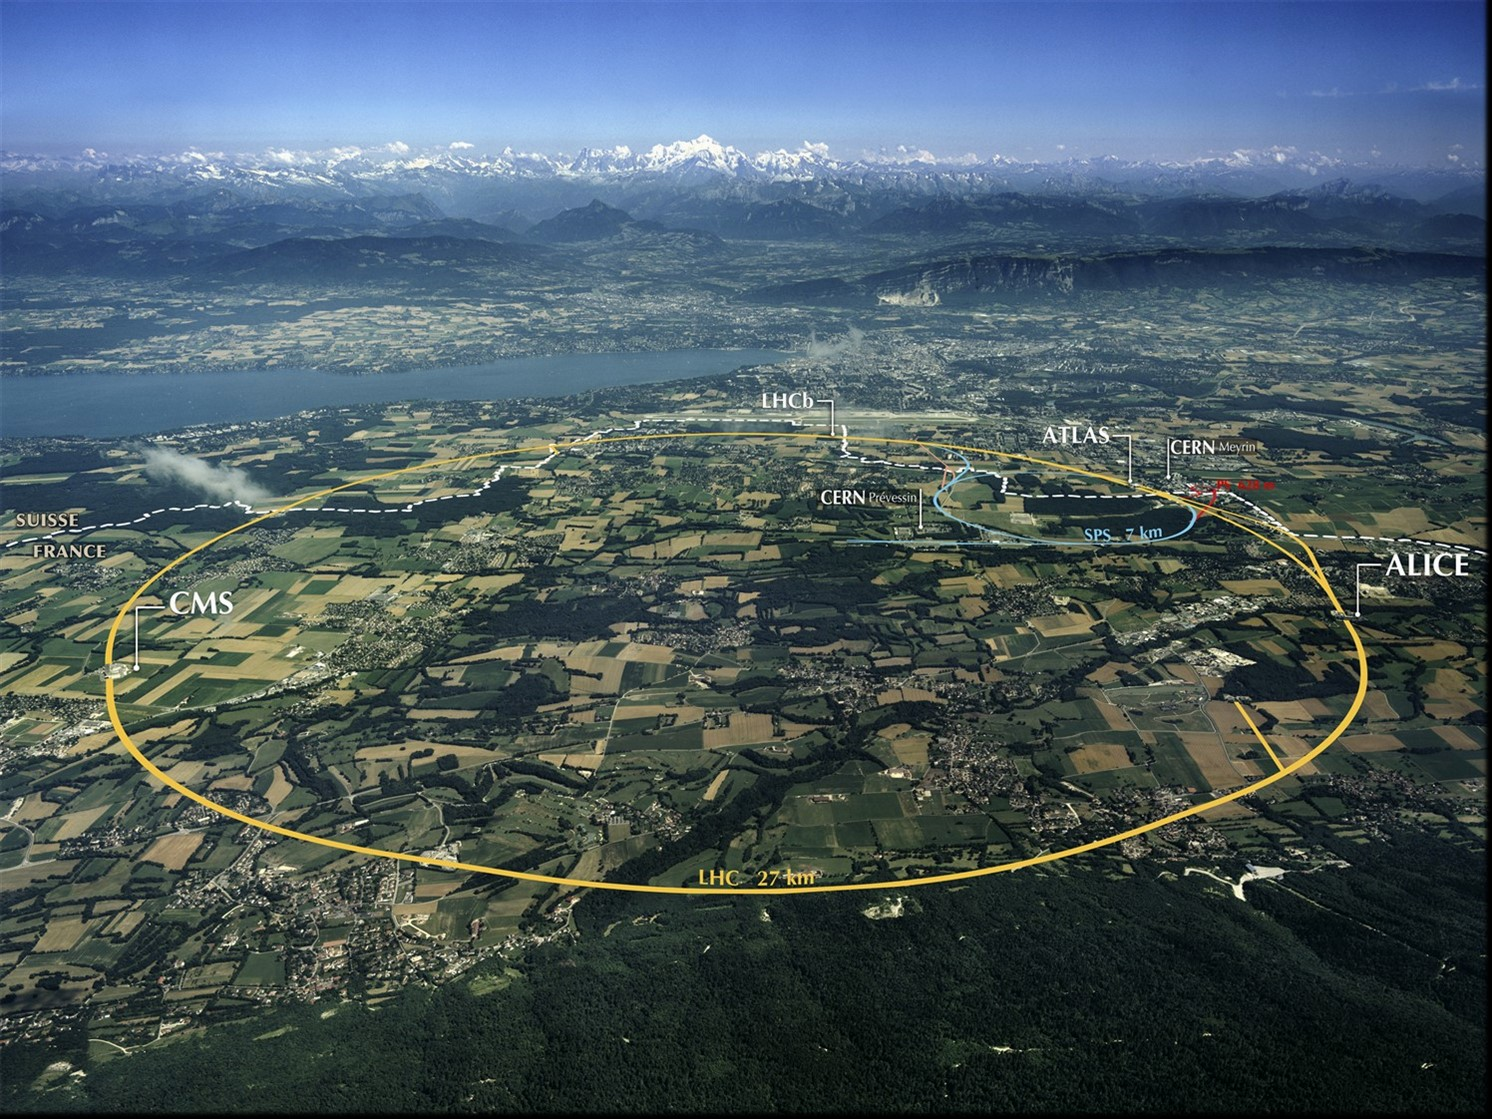
\includegraphics[width=\textwidth]{figures/LHC.jpg}
  \end{columns}

      \begin{itemize}
  \item Still open questions in particles physics remain unanswered:
    \begin{itemize}
    \item Full understanding of the Higgs boson
    \item The origin of matter-antimatter asymmetry
    \item Dark matter
    \item Many more questions ...
    \end{itemize}

  \item Several approaches of high-energy particle colliders to
    address the unanswered questions in the post-LHC era:
    \begin{itemize}
    \item electron-positron ($e^+e^-$) colliders
      \\
      \textcolor{Red}{and/or}
      \\
    \item proton-proton ($p~p$) colliders
    \end{itemize}
  \end{itemize}

\end{frame}

%%%%%%%%%%%%%%%%%%%%%%%%%%%%%
%         SLIDE             %
%%%%%%%%%%%%%%%%%%%%%%%%%%%%%
\begin{frame}
  \frametitle{Hadron vs. Lepton colliders}

  \begin{columns}[t]
    \column{0.5\textwidth}
    \centering
    \begin{tikzpicture}
      \node[anchor=south west,inner sep=0] (image) at (0,
      0){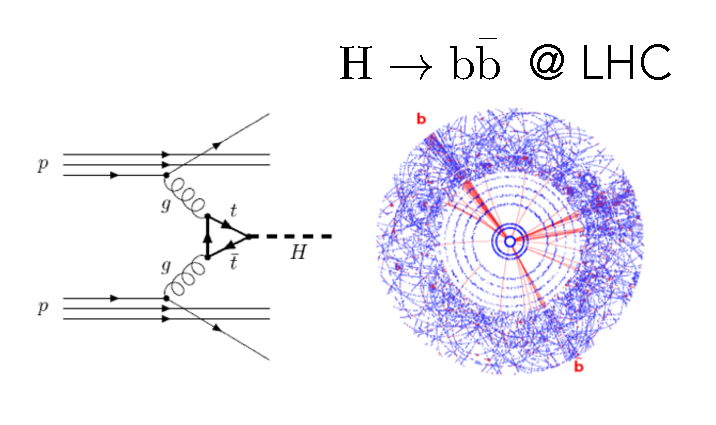
\includegraphics[width=\textwidth]{figures/hadronColliders.pdf}};
      \begin{scope}[x={(image.south east)},y={(image.north west)}]
        \node[above, color=Green, rotate=90] at (0.0, 0.5) {\textbf{Discovery}};
      \end{scope}
    \end{tikzpicture}
    

    \column{0.5\textwidth}
    \centering
    \begin{tikzpicture}
      \node[anchor=south west,inner sep=0] (image) at (0,
      0){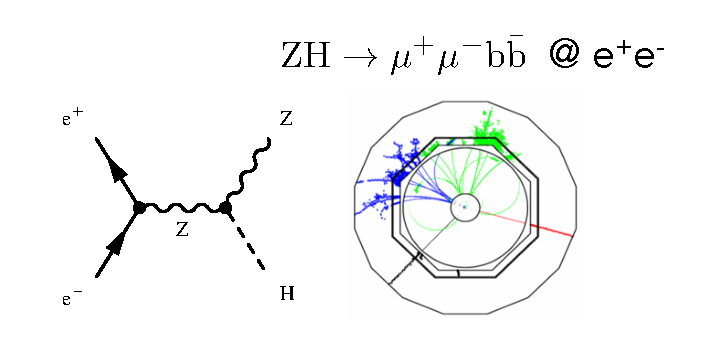
\includegraphics[width=\textwidth]{figures/leptonColliders.pdf}};
      \begin{scope}[x={(image.south east)},y={(image.north west)}]
        \node[above, color=Green, rotate=-90] at (0.9, 0.5) {\textbf{Precision}};
      \end{scope}
    \end{tikzpicture}
  \end{columns}

  \vspace{-0.3cm}

  \begin{columns}[t]
    \column{0.5\textwidth}

    \begin{itemize}
    \item Protons $\Rightarrow$ compound objects
      \begin{itemize}
      \item Unknown event-by-event initial states
      \item Limited achievable precision
      \end{itemize}
    \item High rates of QCD backgrounds
      \begin{itemize}
      \item Complex triggering schemes
      \item High levels of radiation
      \end{itemize}
    %\item High cross-sections for coloured-states
    \item High-energy circular pp colliders are feasible
    \end{itemize}

    \column{0.5\textwidth}

    \begin{itemize}
    \item Electrons/positrons $\Rightarrow$ point-like
      \begin{itemize}
      \item Well-defined initial states (energy, polarisation)
      \item High-precision measurements
      \end{itemize}
    \item Cleaner experimental environment
      \begin{itemize}
      \item Trigger-less readout
      \item Low levels of radiation
      \end{itemize}
    %\item Superior sensitivity for electro-weak states
    \item High-energy $e^+e^-$ collisions ($>350\,\gev$) require
      linear colliders
    \end{itemize}

  \end{columns}

\end{frame}

\section{The Compact Linear Collider (CLIC)}
\begin{frame}
  \frametitle{}
  \tableofcontents[currentsection]
\end{frame}
%%%%%%%%%%%%%%%%%%%%%%%%%%%%%
%         SLIDE             %
%%%%%%%%%%%%%%%%%%%%%%%%%%%%%
{
  \usebackgroundtemplate{
    \begin{picture}(100, 265)
      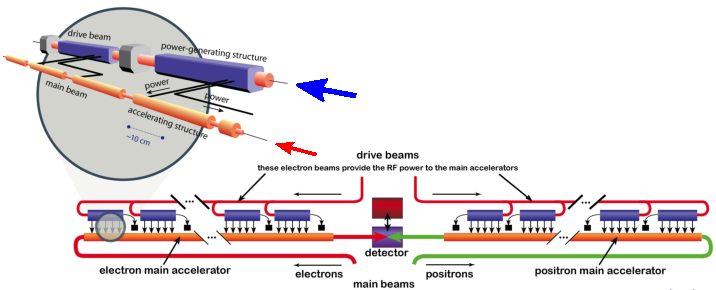
\includegraphics[width=0.9\textwidth]{figures/CLIC_2beam_accel.pdf}
    \end{picture}
  }%
  \begin{frame}
    \frametitle{The Compact Linear Collider (CLIC)}

    \vspace{-1cm}
    \begin{columns}
      \column{0.6\textwidth}
      \begin{itemize}
      \item An $e^{+}e^{-}$ linear collider for the post HL-LHC period.
      \item Energy range $\sqrt{s}$ : \textcolor{Green}{$380\,\gev$} to
        \textcolor{Green}{$3\,\tev$}
        % \begin{itemize} 
        % \item Two-beam acceleration scheme with gradients of $\sim$100~MV/m.
        % \end{itemize}
      \item Precision measurements of:
        \begin{itemize}
        \item Standard Model processes (Higgs, top).
        \item New physics potentially discovered at 13~TeV LHC.
        \item Search for new physics
          % : unique sensitivity to particles with electroweak charge.
        \end{itemize}
      \item 50~km tunnel at 3~TeV stage
      \end{itemize}
      
      \column{0.4\textwidth}
      \centering
      \includegraphics[width=1.1\textwidth]{../figures/CLIC/staging.pdf}
    \end{columns}

    %\vspace{-0.3cm}
    \begin{columns}[t]
      \column{0.5\textwidth}
      \begin{itemize}
      \item Two-beam acceleration scheme
      \end{itemize}
      \column{0.5\textwidth}
      \begin{itemize}
      \item \textcolor{blue}{Drive beam $\Rightarrow$ RF power}
        \begin{itemize}
        \item 12~GHz bunch structure
        \item High current 100~A
        \item Low energy $2.4\,\gev$ - $240\,\gev$
        \end{itemize}
      \item \textcolor{red}{Main beam $\Rightarrow$ physics}
        \begin{itemize}
        \item Lower current 1.2~A
        \item High energy $9\,\gev$ - $1.5\,\tev$
        \end{itemize}
      \end{itemize}
    \end{columns}

  \end{frame}
}


%%%%%%%%%%%%%%%%%%%%%%%%%%%%%
%         SLIDE             %
%%%%%%%%%%%%%%%%%%%%%%%%%%%%%
\begin{frame}
  \frametitle{Experimental conditions at CLIC}
  
 \begin{columns}
   \column{0.6\textwidth}

   \begin{itemize}
   \item Beam profile:
     \begin{itemize}
     \item Bunch crossings (BX): every 0.5~ns.
     \item Train duration: 156~ns (312 bunches).
     \item Train repetition: 20~ms (50~Hz).
     \end{itemize}
     $\Rightarrow$ \textcolor{blue}{Triggerless readout} \&
     \textcolor{blue}{power pulsing}
   \end{itemize}

   \column{0.4\textwidth}
   \begin{tikzpicture}
     \node[anchor=south west,inner sep=0] (image) at (0,
     0){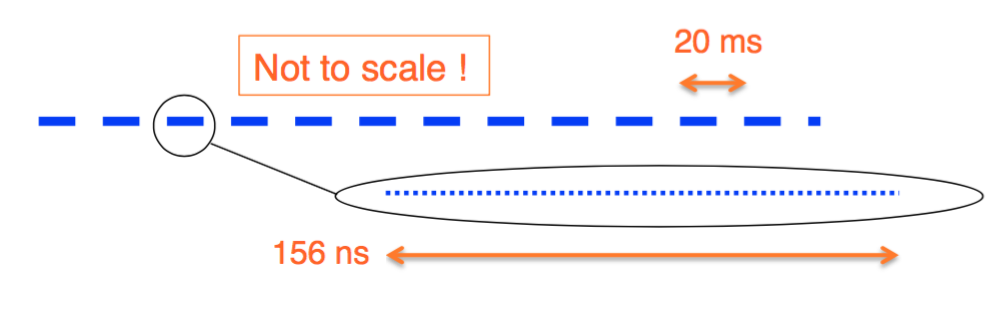
\includegraphics[width=\textwidth]{figures/CLICbeam.png}};
     \begin{scope}[x={(image.south east)},y={(image.north west)}]
       \node[above, color=blue] at (0.5, 0.9) {\textbf{CLIC bunch
           structure}};
     \end{scope}
   \end{tikzpicture}
 \end{columns}
 
 \vspace{0.5cm}
 \centering
 \resizebox{0.9\columnwidth}{!}{\begin{tabular}{l c c} 
                                  \toprule 
                                  & CLIC at $\sqrt{s}=3\,\tev$ & LHC at $\sqrt{s}=13\,\tev$\\
                                  \midrule
                                  Instantaneous luminosity $\mathcal{L}$ & $6\times10^{34}$ \inversecmsquaredsec & $1\times10^{34}$ \inversecmsquaredsec \\
                                  Bunch-crossing separation & 0.5~ns & 25~ns \\
                                  IP size in x / y / z directions & 45~nm / 1~nm / $44\,\micron$ & $15\,\micron$ / $15\,\micron$ / 5~cm \\
                                  \bottomrule
                                \end{tabular}
}
                              
                              % \column{0.5\textwidth}
                              % \centering


%\vspace{0.3cm}



  \begin{columns}
    \column{0.7\textwidth}
    \begin{itemize}
    \item Beam-induced backgrounds (small beam sizes):
      \begin{itemize}
      \item Beamstrahlung: $\gamma\gamma$ $\rightarrow$
        $e^{+}e^{-}$/hadrons
      \item Forward direction
      \item Timing cuts to reduce the effect
      \end{itemize}
    \end{itemize}
    
    \column{0.3\textwidth}    
    \centering
    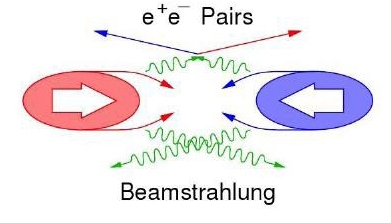
\includegraphics[width=\textwidth]{figures/beamstrahlung.png}
  \end{columns}

  \begin{itemize}
  \item Each train consists of:
    \begin{itemize}
    \item At most 1 interesting event.
    \item $>$ 30000 background particles inside the detector.
    \end{itemize}
  \item Moderate exposure to radiation: by a factor of $10^4$ less
    than the LHC.
  \end{itemize}
\end{frame}


%%%%%%%%%%%%%%%%%%%%%%%%%%%%%
%         SLIDE             %
%%%%%%%%%%%%%%%%%%%%%%%%%%%%%
\begin{frame}
  \frametitle{The CLIC detector}

  % \begin{columns}
  %   \column{0.5\textwidth}
  \centering
  \begin{tikzpicture}
    \node[anchor=south west,inner sep=0] (image) at (0,
    0){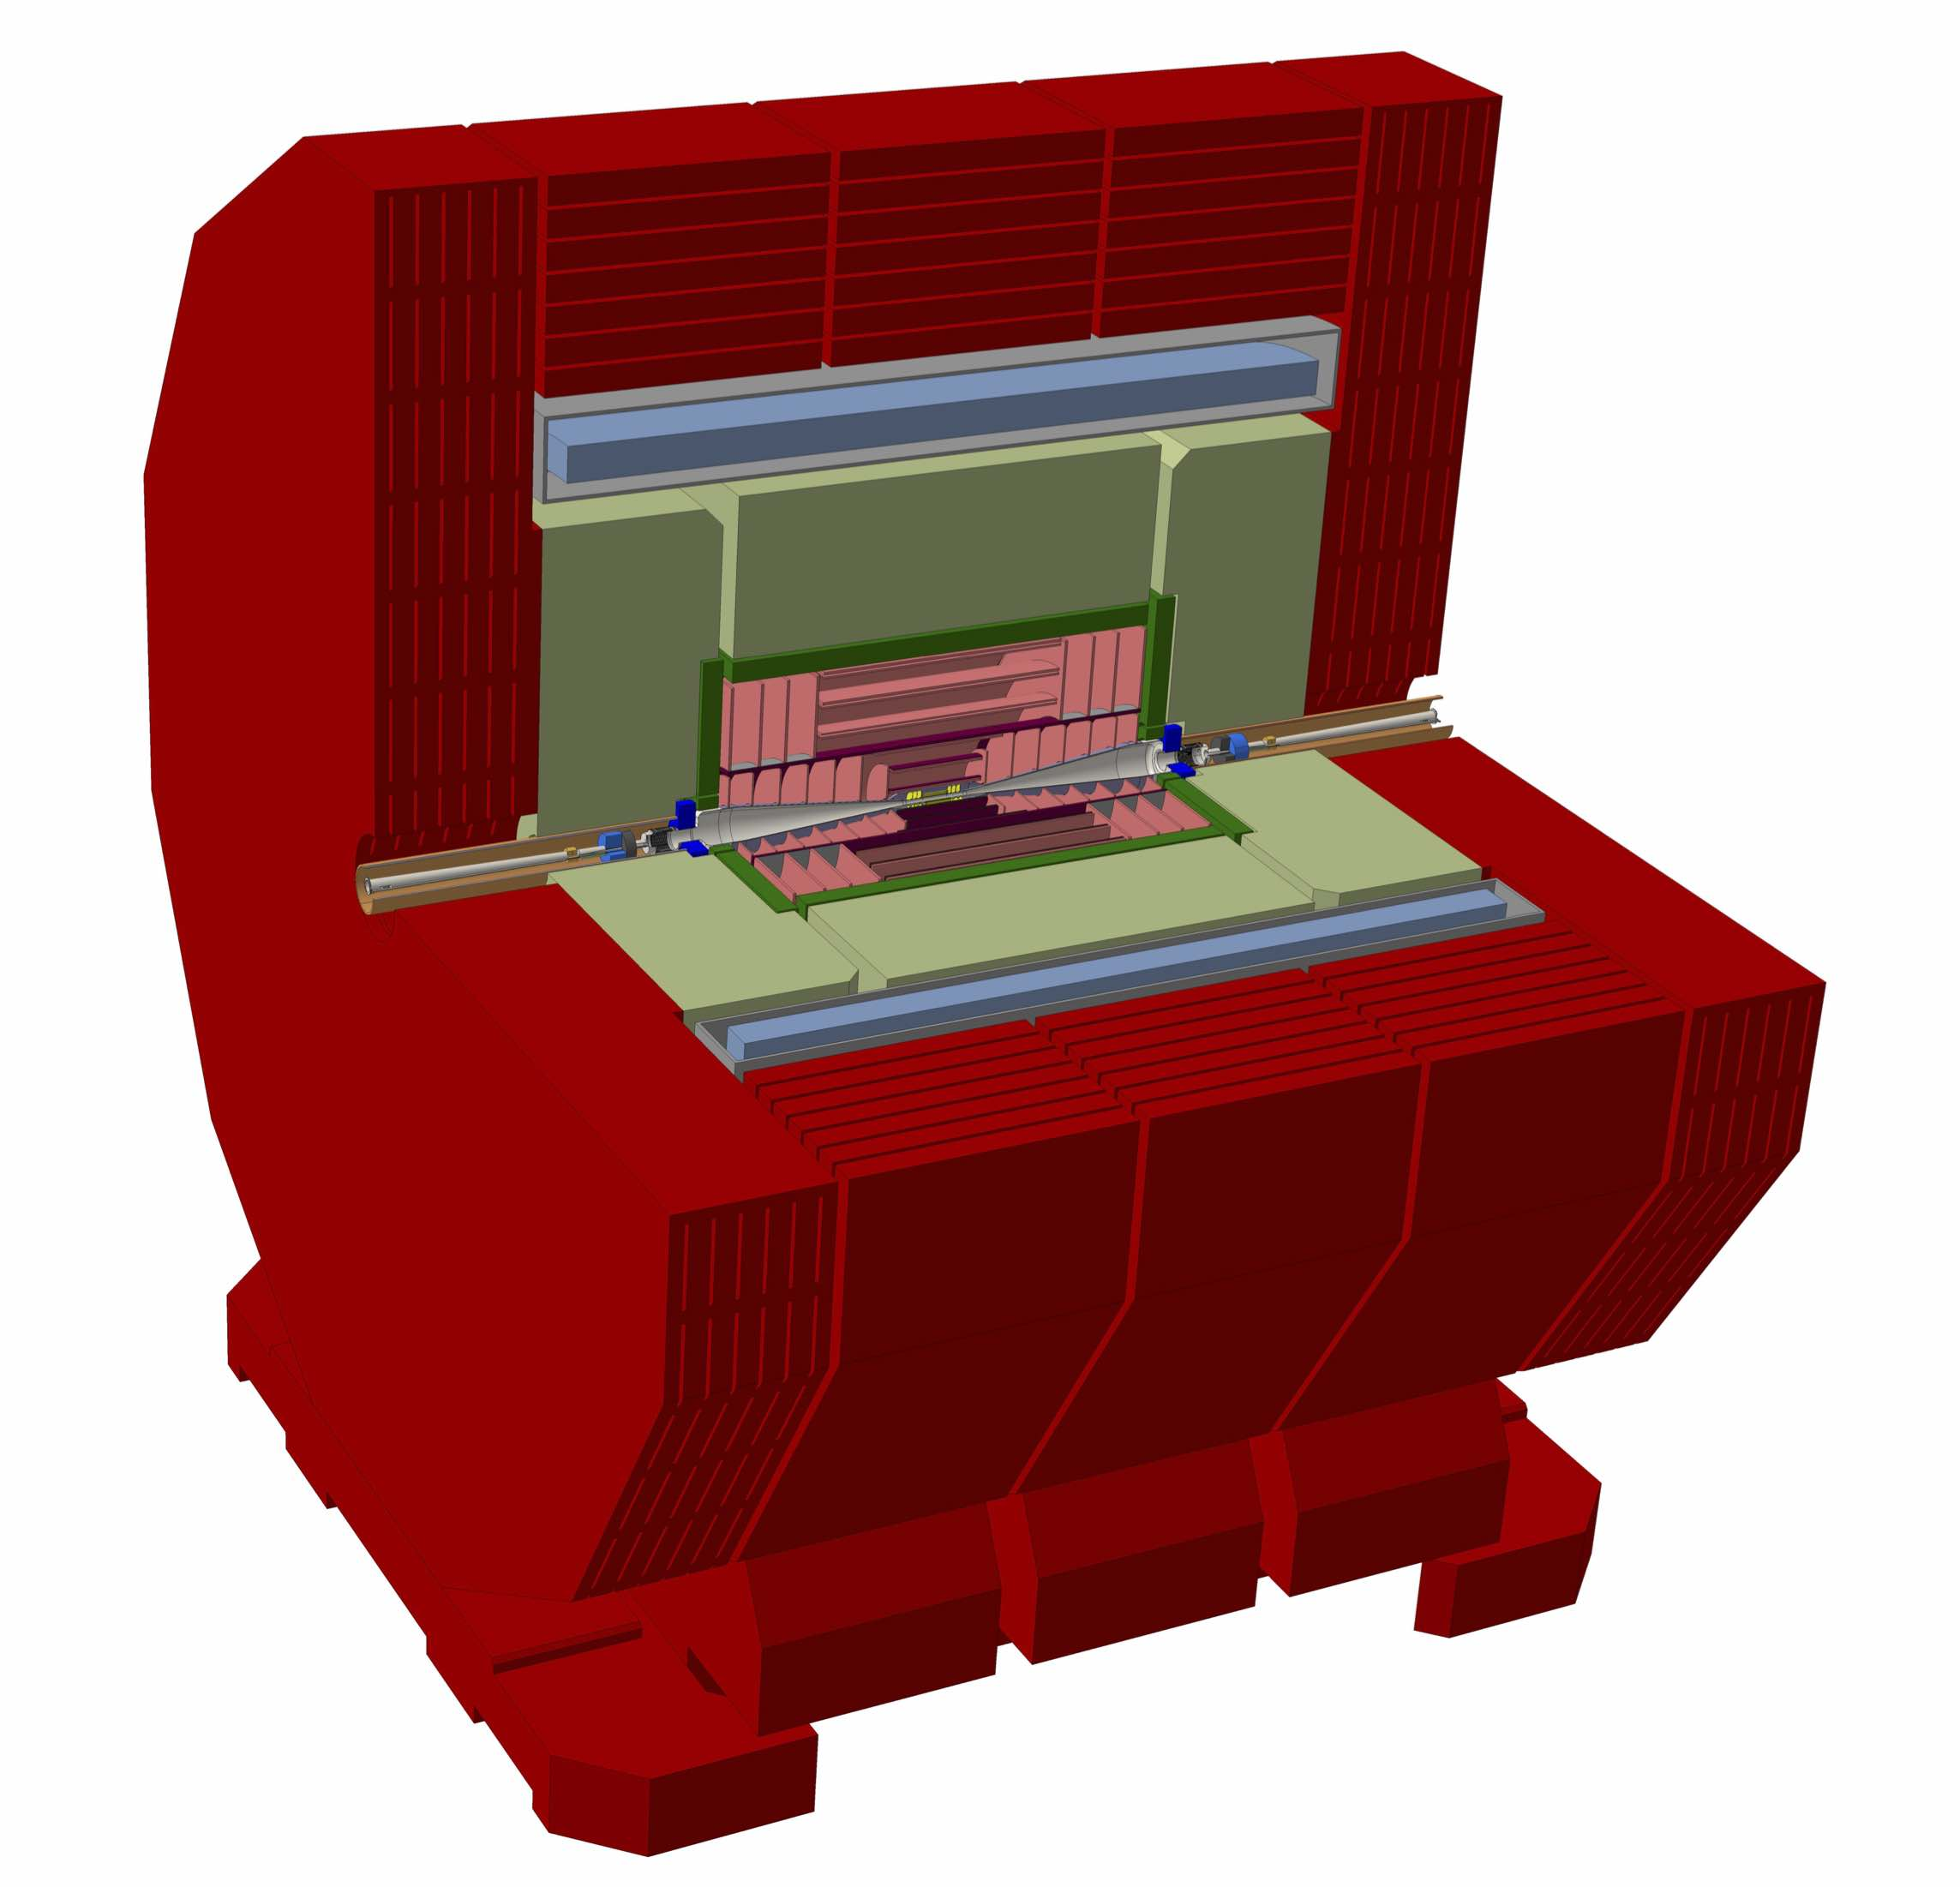
\includegraphics[width=0.8\textwidth]{figures/CLIC_detector_2016.jpg}};
    \begin{scope}[x={(image.south east)},y={(image.north west)}]

      % \draw[help lines,xstep=.1,ystep=.1] (0, 0) grid (1,1);
      % \foreach \x in {0,1,...,9} { \node [anchor=north] at (\x/10,0) {0.\x}; }
      % \foreach \y in {0,1,...,9} { \node [anchor=east] at (0,\y/10)
      % {0.\y}; }

      \draw[<->,line width=0.5pt] (0.32, 0.0) -- (0.8, 0.13);
      \node[color=black] at (0.6, 0.02) {11.4~m};

      \draw[<->,line width=0.5pt] (0.04, 0.17) -- (0.04, 0.9);
      \node[color=black, rotate=90] at (0.01, 0.5) {12.9~m};

      \node[text width=2.5cm, color=black] at (1, 0.58)
      {Silicon-based tracking system};
      \draw[->,line width=0.7pt] (0.8, 0.6) -- (0.5, 0.6);

      \node[text width=3cm, color=black] at (1, 0.7) {Calorimetry
        system: ECAL and HCAL};
      \draw[->,line width=0.7pt] (0.8, 0.72) -- (0.5, 0.72);

      \node[text width=4cm, color=black] at (1.05, 0.85) {Superconducting
        solenoid magnet};%: B=4~T};
      \draw[->,line width=0.7pt] (0.8, 0.85) -- (0.6, 0.8);

      \node[text width=4cm, color=black] at (1.1, 0.2) {Forward
        region: \\ LumiCal \& BeamCal};
      \draw[->,line width=0.7pt] (0.85, 0.2) -- (0.3, 0.55);

      \node[text width=3cm, color=white] at (0.45, 0.25) {Return iron
        yoke with detectors for muon identification};
    \end{scope}
  \end{tikzpicture}

  %   \column{0.5\textwidth}
  %   \begin{itemize}
  %   \item Composed of several sub-detectors.
  %   \item Silicon-based and low mass tracking system.
  %   \item Fine-grained calorimetry system (ECAL and HCAL) optimised
  %     for particle flow analysis (PFA).
  %   \item Superconducting solenoid magnet: B=4~T.
  %   \item Return iron yoke with detectors for muon identification.
  %   \item Forward region with LumiCal (luminosity monitoring) and
  %     BeamCal (beam calorimeter).
  %   \end{itemize}

  % \end{columns}

\end{frame}

\section{The CLIC vertex detector}
\begin{frame}
  \frametitle{}
  \tableofcontents[currentsection]
\end{frame}
%%%%%%%%%%%%%%%%%%%%%%%%%%%%%
%         SLIDE             %
%%%%%%%%%%%%%%%%%%%%%%%%%%%%%
\begin{frame}
  \frametitle{The CLIC vertex detector}

  \begin{columns}
    \column{0.75\textwidth}
    \textcolor{Red}{\textbf{Goal}}: Efficient tagging of heavy quarks
    through a precise determination of displaced vertices.

    \column{0.25\textwidth}

    \centering
    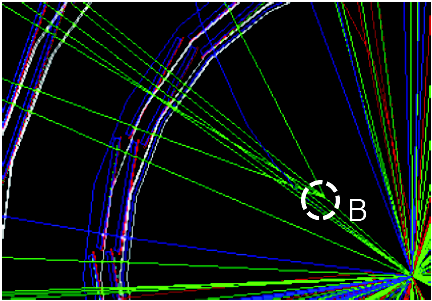
\includegraphics[width=\textwidth]{figures/secondary_vertex.png}
  \end{columns}



  \begin{columns}
    \column{0.6\textwidth}

    \begin{itemize}
    \item Requirements:
      \begin{itemize}
      \item Multi-layer: 
        \begin{itemize}
          \item 6 layers in the barrel and 6 disks
          \end{itemize}
      \item Large angular coverage: 
        \begin{itemize}
        \item $\sim30$~mm of inner radius and
          $\theta_{min}\sim8^{\circ}$
        \end{itemize}
      \item B-field: \textcolor{Blue}{4~T}
      \item Hit resolution of
        \textcolor{Blue}{$\sim$\SI{3}{\micro\meter}}
        \begin{itemize}
        \item Pixel detectors
        \end{itemize}
      \item Low material budget: 
        \begin{itemize}
        \item $<0.2\%$~X\textsubscript{0}/layer
        \item Forced airflow cooling
        \item Low-power electronics
          ($\approx 50$~mW/cm\textsuperscript{2})
        \end{itemize}
      \item Time slicing of
        \textcolor{Blue}{$\sim$\SI{10}{\nano\second}}
        \begin{itemize}
        \item reject out of time background.
        \end{itemize}
        % \begin{itemize}
        % \item high-resistive \& depleted sensors
        % \item readout with precise timing.
        % \end{itemize}
      \end{itemize}
    \end{itemize}

    \column{0.4\textwidth}
    \centering
    % \begin{tikzpicture}
    %   \node[anchor=south west,inner sep=0] (image) at (0,
    %   0){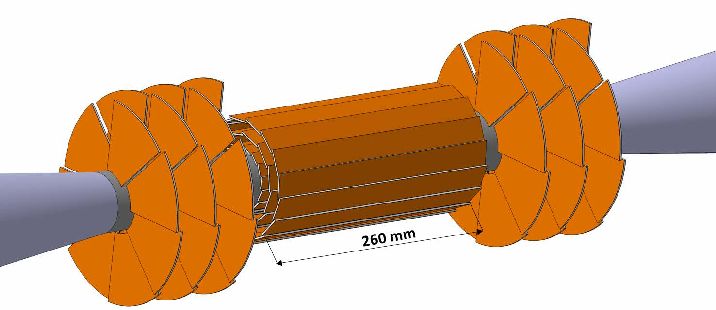
\includegraphics[width=\textwidth]{figures/spiralVXD.pdf}};
    %   \begin{scope}[x={(image.south east)},y={(image.north west)}]
    %     \draw[<->, Blue, thick](0.2, 0.0)--(0.84, 0.2);
    %     \node[below, color=Blue] at (0.5, 0.05) {56 cm};
    %   \end{scope}
    % \end{tikzpicture}

    \begin{tikzpicture}
      \node[anchor=south west,inner sep=0] (image) at (0,
      0){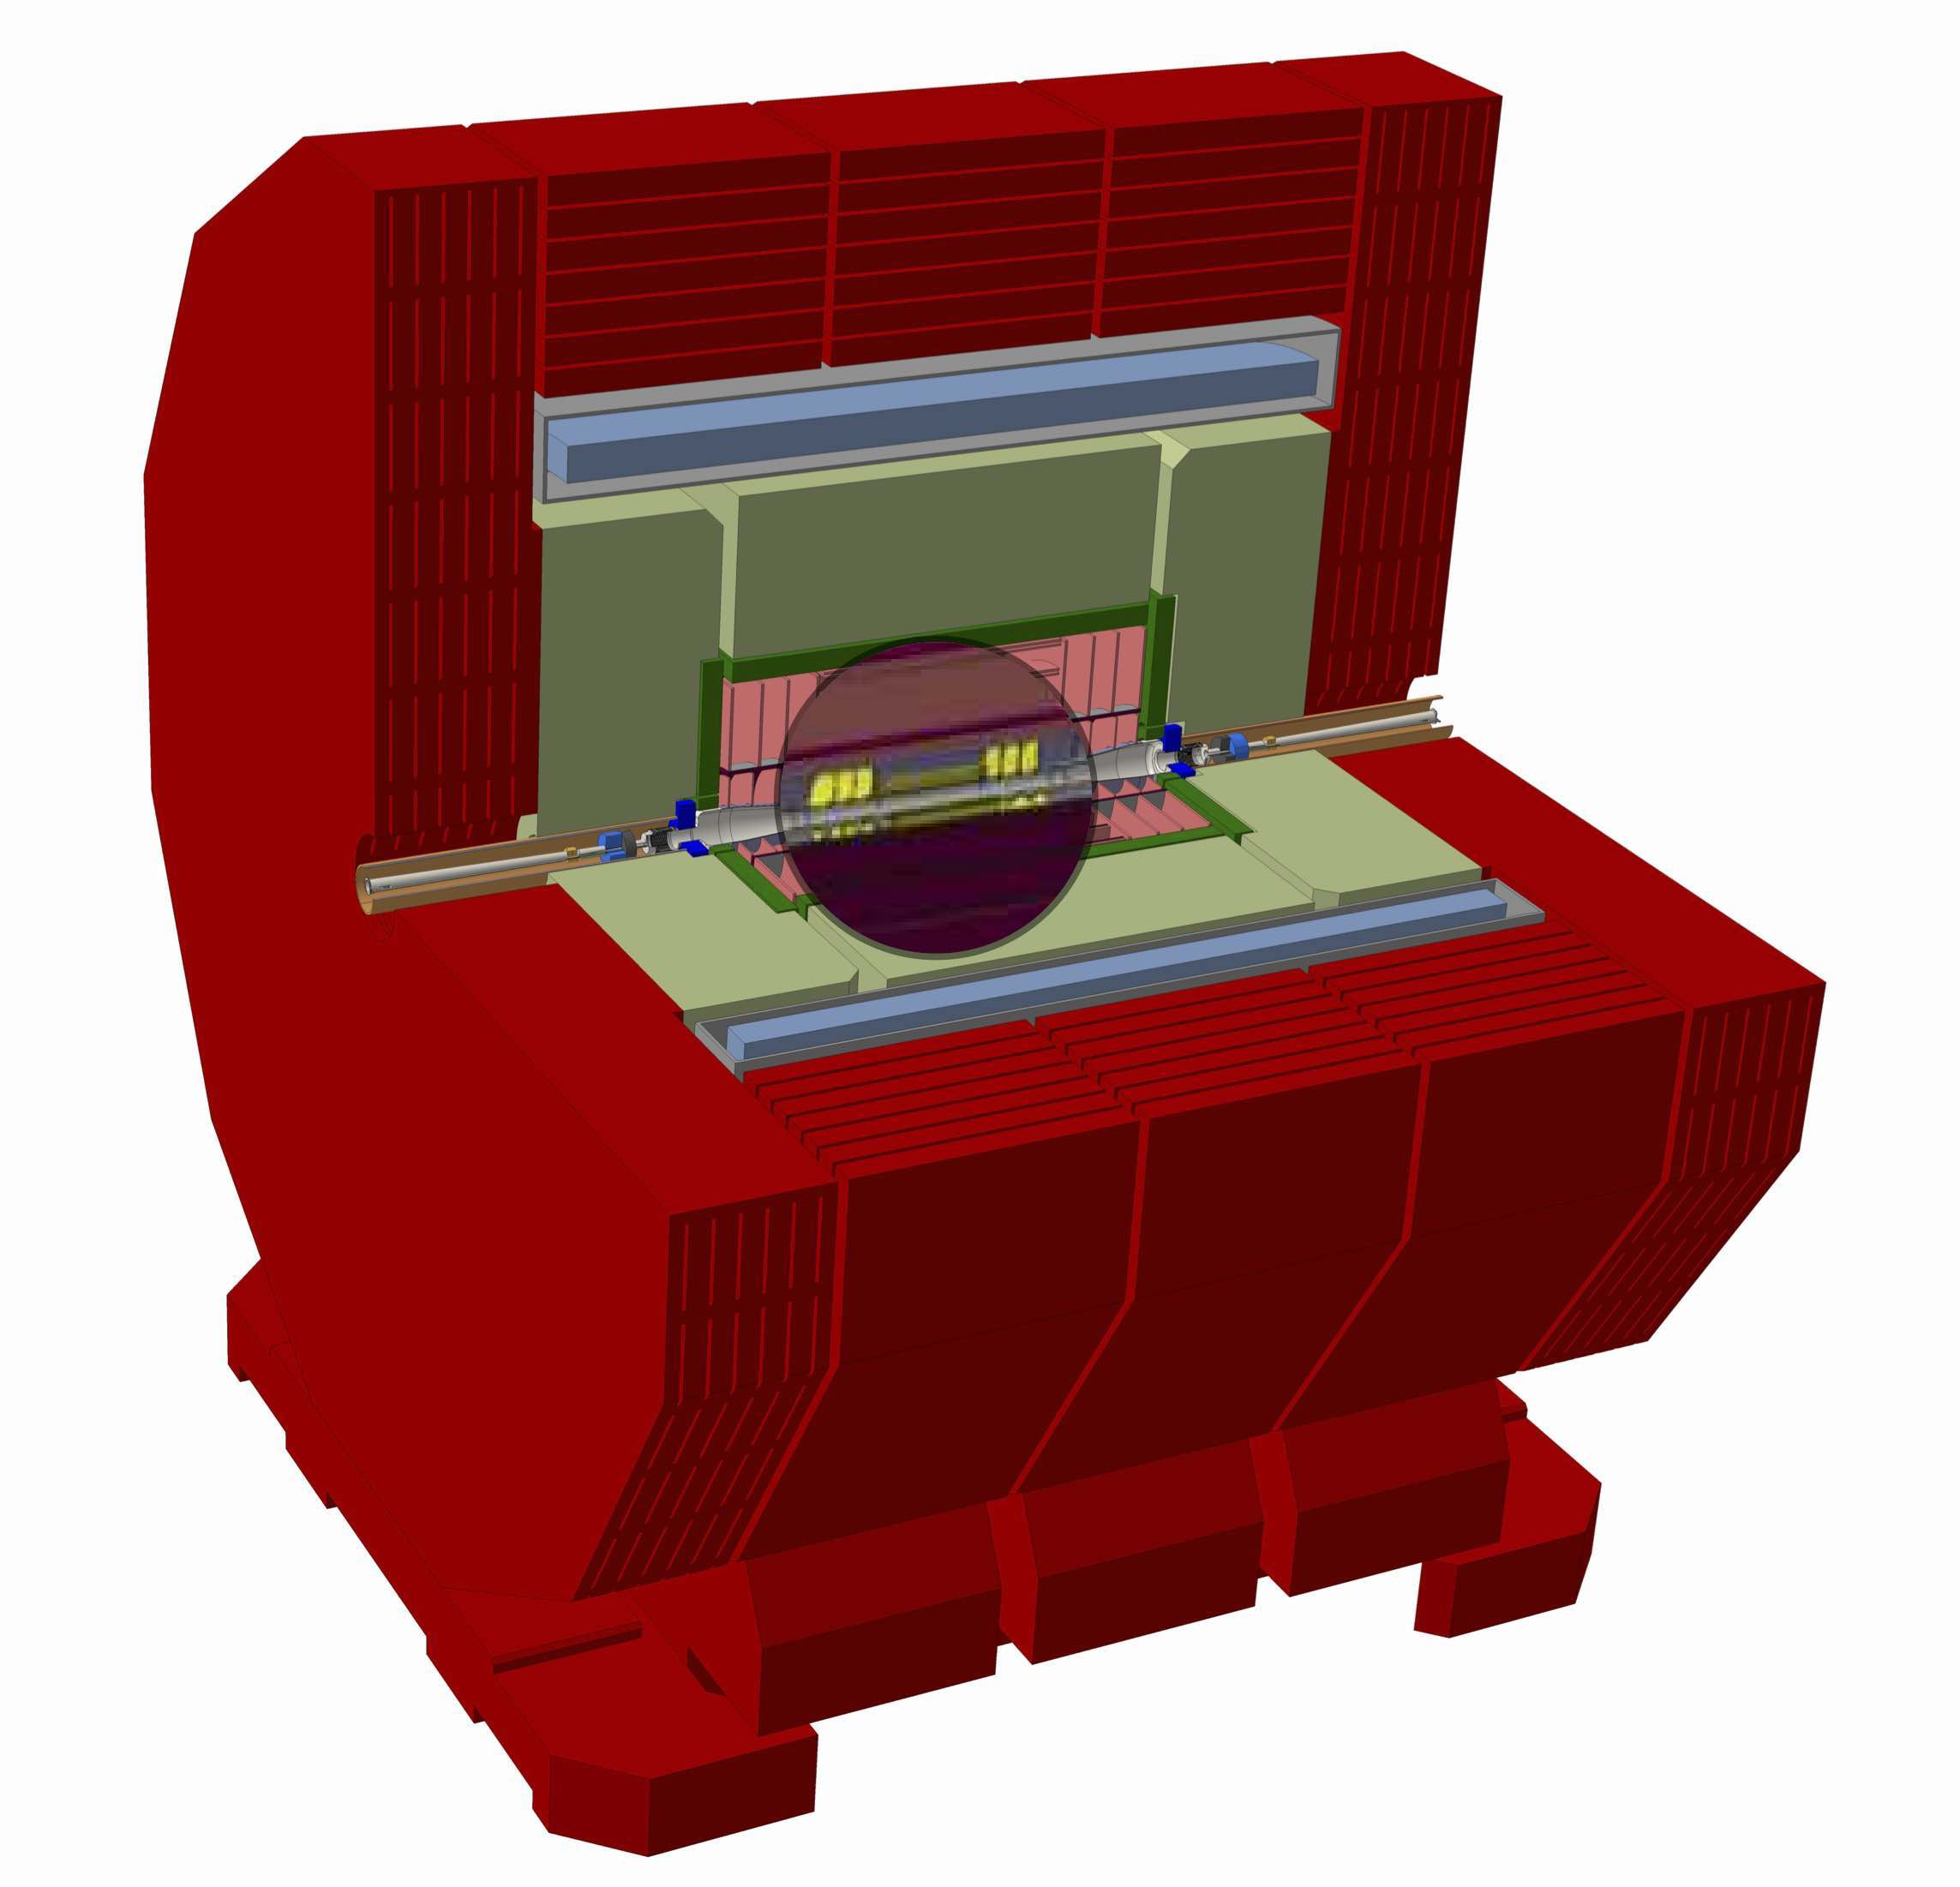
\includegraphics[width=\textwidth]{figures/CLIC_detector_2016_zoomVertex}};
      \begin{scope}[x={(image.south east)},y={(image.north west)}]
        
        % \draw[help lines,xstep=.1,ystep=.1] (0, 0) grid (1,1);
        % \foreach \x in {0,1,...,9} { \node [anchor=north] at (\x/10,0) {0.\x}; }
        % \foreach \y in {0,1,...,9} { \node [anchor=east] at (0,\y/10)
        % {0.\y}; }

        % \draw[<->,line width=0.5pt] (0.15, 0.95) -- (0.7, 0.99);
        % \node[color=black] at (0.45, 1) {11.4~m};
       
        
        % \node[color=white] at (0.45, 0.9) {\textbf{CLIC detector}};
        \draw[->,line width=1.7pt] (0.5, 0.5) -- (0.5, -0.05);
        % \node[color=black] at (0.58, 0.43) {\textbf{VXD}};

      \end{scope}
    \end{tikzpicture}

    \vspace{-0.5cm}
    \begin{tikzpicture}
      \node[anchor=south west,inner sep=0] (image) at (0,
      0){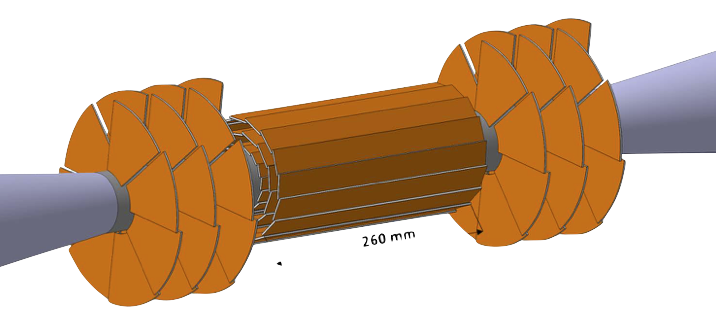
\includegraphics[width=\textwidth]{figures/spiralVXD_2.png}};
      \begin{scope}[x={(image.south east)},y={(image.north west)}]
        \draw[<->, Blue, thick](0.2, 0.0)--(0.84, 0.2);
        \node[below, color=Blue] at (0.5, 0.05) {56 cm};
      \end{scope}
    \end{tikzpicture}

  \end{columns}


\end{frame}

%%%%%%%%%%%%%%%%%%%%%%%%%%%%%
%         SLIDE             %
%%%%%%%%%%%%%%%%%%%%%%%%%%%%%
\begin{frame}
  \frametitle{Flavour-tagging at CLIC}

  \begin{columns}
    \column{0.6\textwidth}
    \begin{itemize}
    \item At $\sqrt{s}=3\,\tev$ the production of the $126\,\gev$
      Higgs
      boson is dominated by the process: \\
      e$^+$e$^- \rightarrow$H$\nu\bar{\nu}$
    \item The Higgs boson decays to b\={b} and c\={c} quark pairs.
    \end{itemize}

    \column{0.4\textwidth}
    \centering
    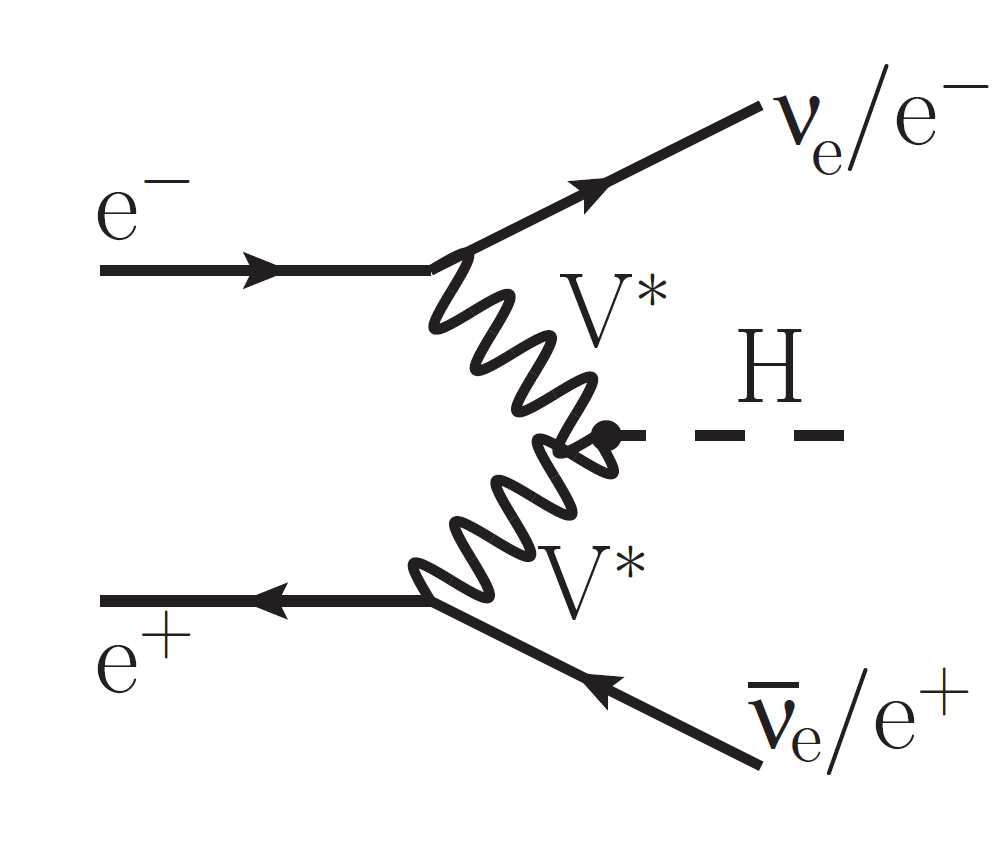
\includegraphics[width=0.5\textwidth]{figures/feynman_higgs.png}
  \end{columns}

  \begin{itemize}
  \item A high-precision vertex detector allows for beauty and
    charm-tagging and to study such decay modes.
  \end{itemize}

  \begin{columns}
    \column{0.5\textwidth}
    \centering
    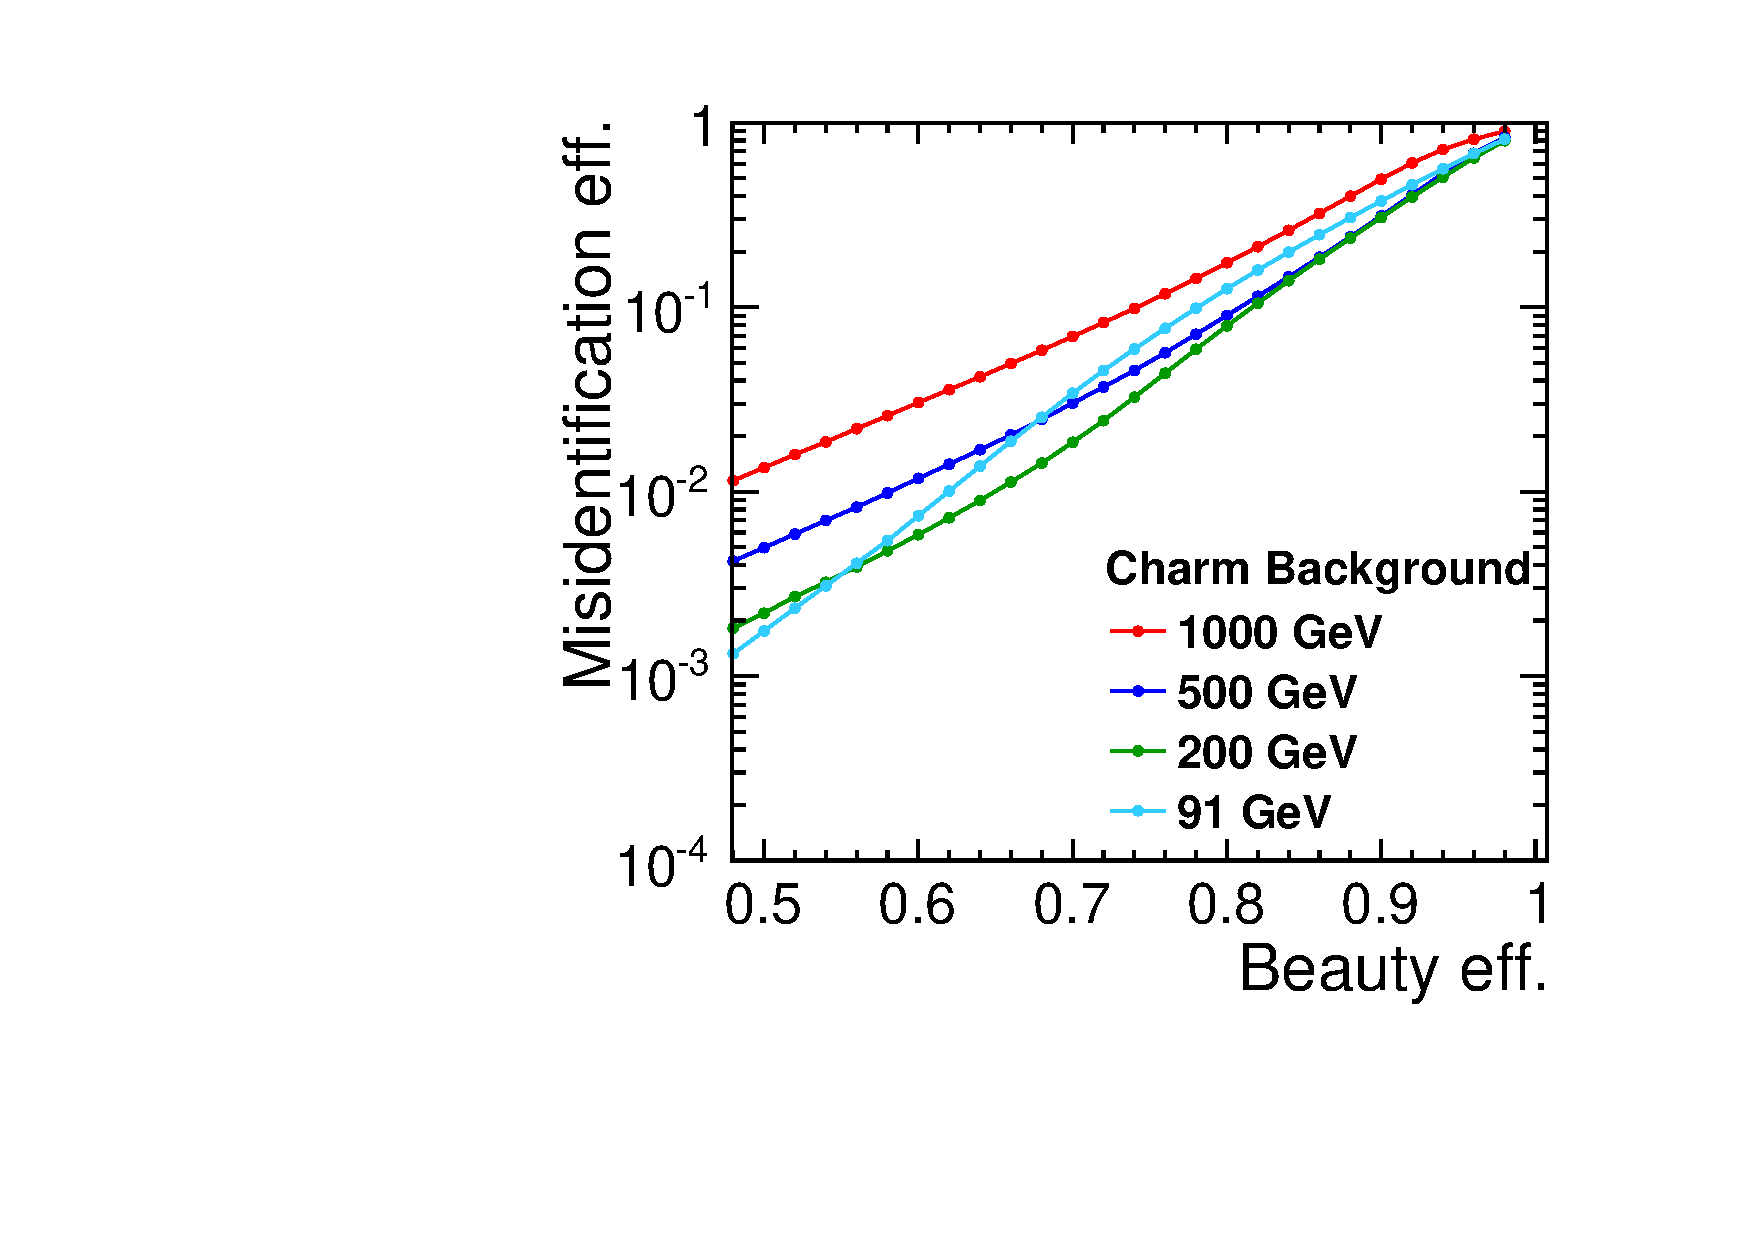
\includegraphics[width=\textwidth]{figures/Global_energies_CLIC_SiD_spirals_Beauty_Charm_.pdf}
    \column{0.5\textwidth}
    \centering
    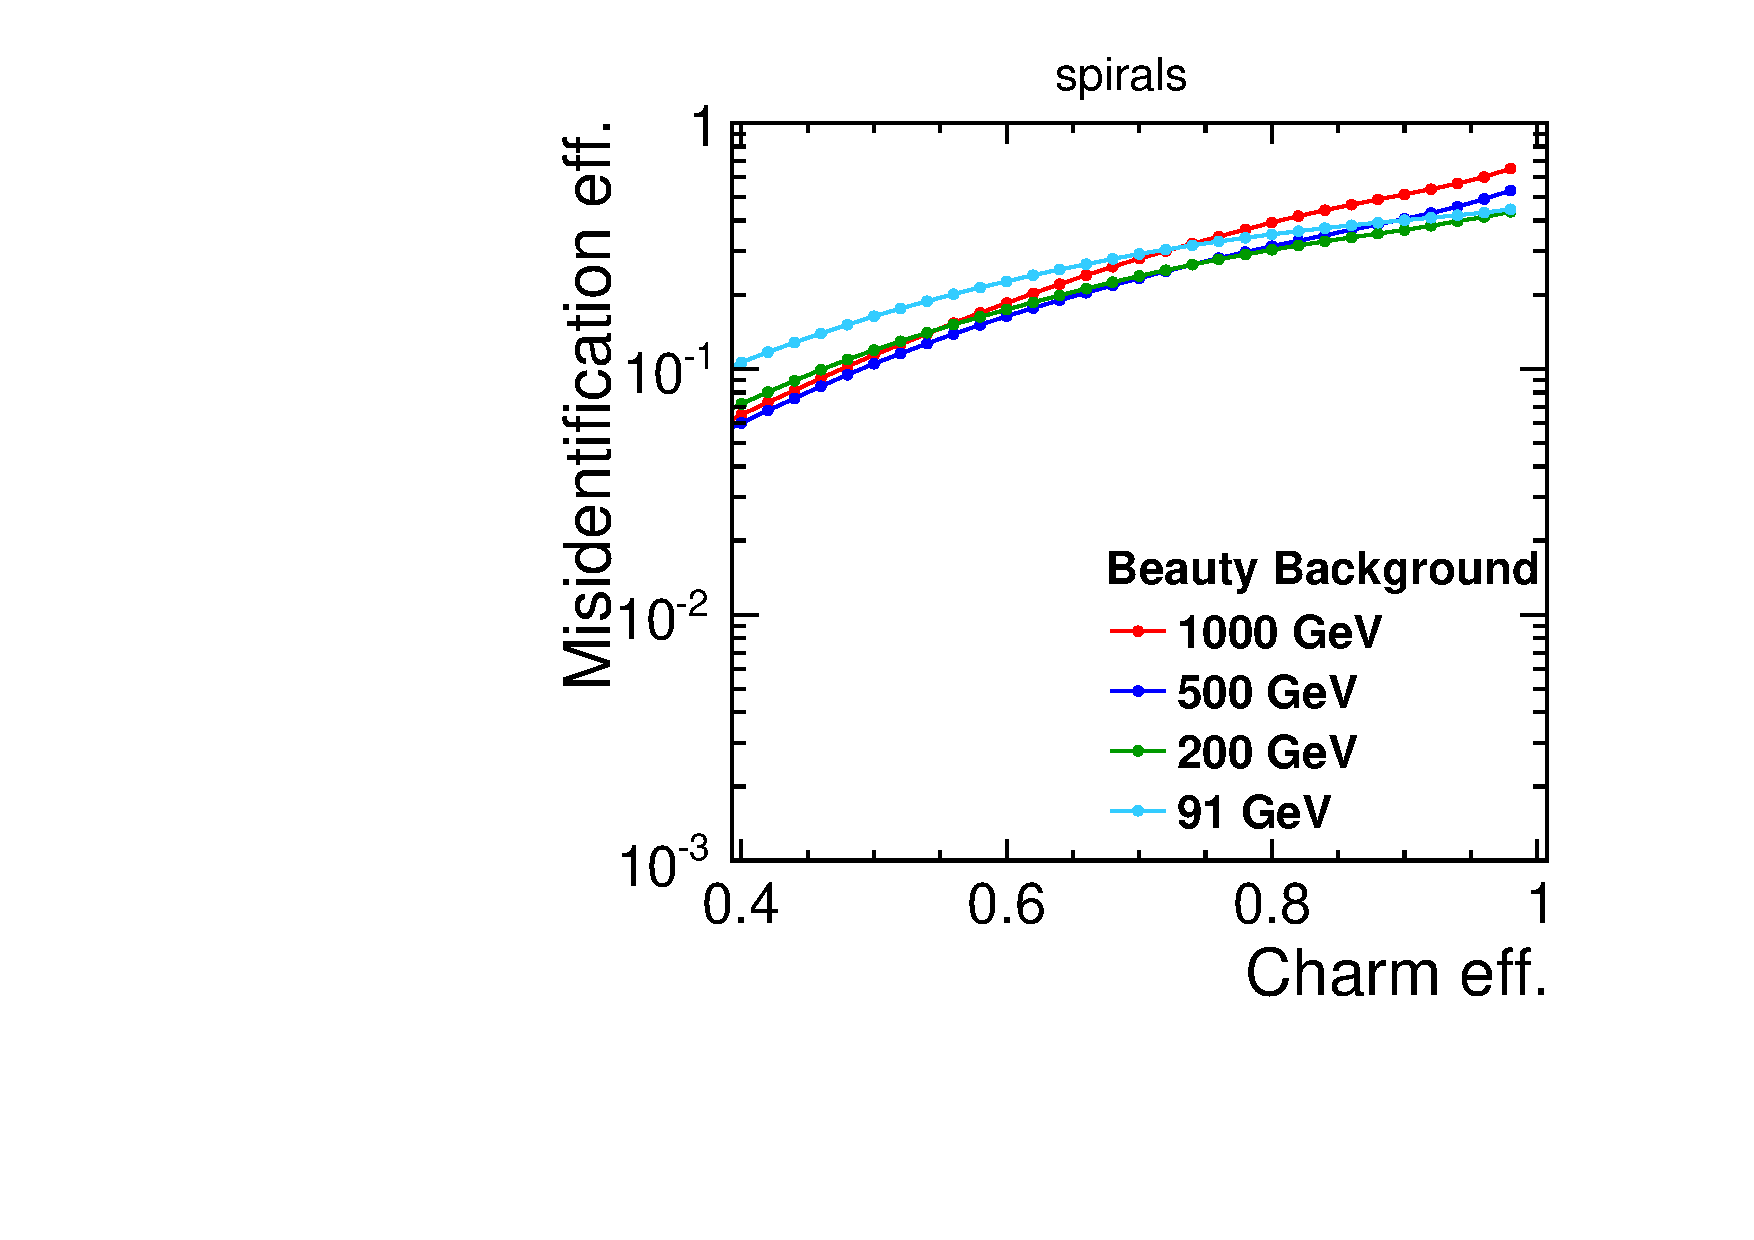
\includegraphics[width=\textwidth]{figures/Global_energies_CLIC_SiD_spirals_Charm_Beauty_.pdf}
  \end{columns}

\end{frame}


\section{R\&D for hybrid pixel detectors at CLIC}
\begin{frame}
  \frametitle{}
  \tableofcontents[currentsection]
\end{frame}
%%%%%%%%%%%%%%%%%%%%%%%%%%%%%
%         SLIDE             %
%%%%%%%%%%%%%%%%%%%%%%%%%%%%%
% ----------------------------- %
\tikzstyle{block} = [rectangle, draw, text width=5.5em, text centered, rounded corners, minimum
height=4em]
\usetikzlibrary{backgrounds,fit,decorations.pathreplacing} 

% ----------------------------- %
\begin{frame}
  \frametitle{R\&D for planar pixel detectors at CLIC}


  \begin{columns}
    \column{0.7\textwidth}
    \begin{itemize}
    \item Planar silicon sensor: reverse-biased pn-junction
      \begin{itemize}
      \item Drift $\Rightarrow$ external electric field
      \item Diffusion $\Rightarrow$ thermal motion
      \item Segmentation \& diffusion $\Rightarrow$ position
        information
      \end{itemize}
    \end{itemize}
    \column{0.3\textwidth}
    \centering

    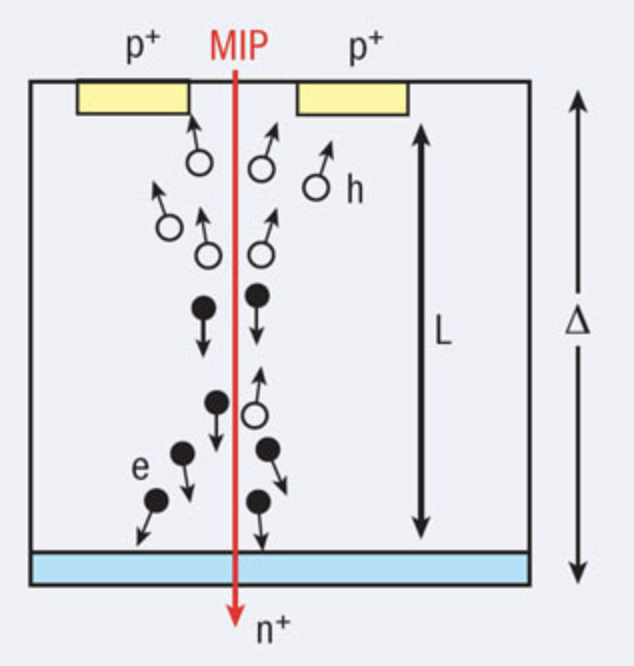
\includegraphics[width=0.8\textwidth]{figures/Diffusion.png}
  \end{columns}

  \vspace{-0.5cm}

  \begin{columns}
    \column{0.6\textwidth}
    \begin{itemize}
    \item \textcolor{Red}{\textbf{Goal}}: achieve $3\,\micron$ hit resolution with:
      \begin{itemize}
      \item Low material $\Rightarrow$ $50\,\micron$-thick sensor \& $50\,\micron$-thick ASICß
      \item Small pixels $\Rightarrow$ $25\,\micron$ pitch
      \item Analogue readout
      \end{itemize}
    \end{itemize}

    \column{0.4\textwidth}
    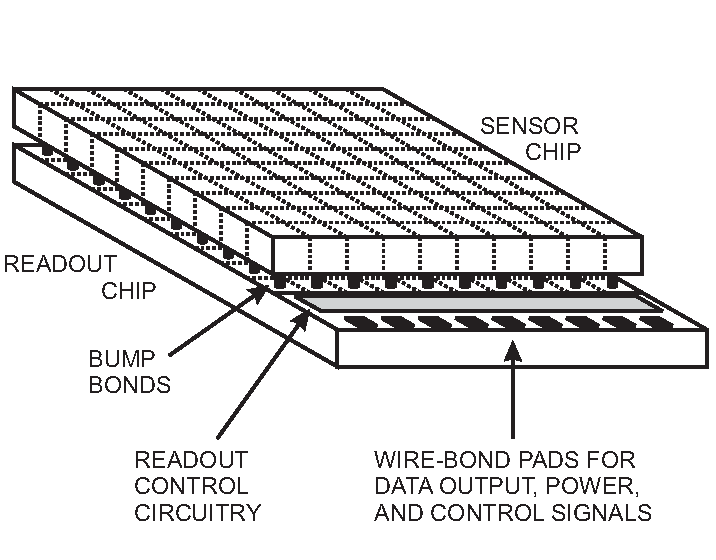
\includegraphics[width=\textwidth]{figures/hybridDet.pdf}
    % \centering
    % \begin{adjustbox}{max totalsize={.9\textwidth}{.9\textheight},center}
    %   \begin{tikzpicture}[node distance = 2.5cm, auto]
    %     \begin{scope}[x={(image.south east)},y={(image.north west)}]
    %       \draw[very thick] (0.1, 0.1) rectangle (0.5, 0.9);
    %       \draw[<->,line width=1pt] (0.1, 1) -- (0.5, 1);
    %       \node[color=black] at (0.3, 1.2) {pitch};

    %       \fill (0.35, 0.6) circle[radius=1pt];
    %       \draw (0.35, 0.6) circle[radius=5pt];

    %       \draw[<->] (0.35, 0.4) -- (0.42, 0.4);
    %       \node[color=black] at (0.38, 0.28) {$\sigma$};

    %     \end{scope}
    %   \end{tikzpicture}
    % \end{adjustbox}

    % \centering
    % 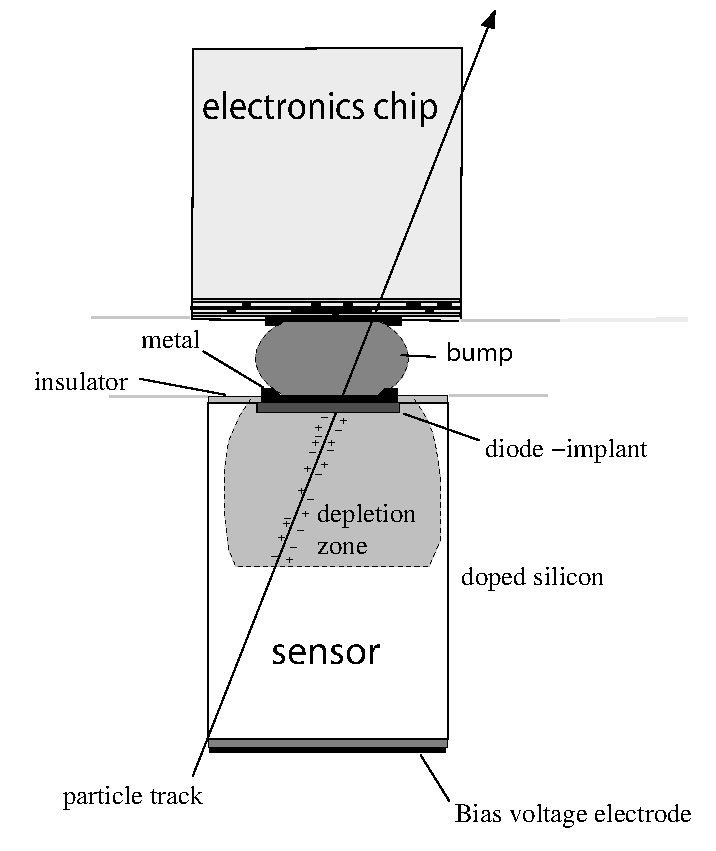
\includegraphics[width=\textwidth]{figures/siliconSensorPrinciple.pdf}

  \end{columns}


  \begin{columns}
    \column{0.7\textwidth}
    \begin{itemize}
    \item Characterisation of thin n-in-p sensors (Advacam) using the
      Timepix3 readout ASIC with \textcolor{Blue}{$55\,\micron$} pixel
      pitch:
      \begin{itemize}
      \item Sensor thicknesses: $50\,\micron$ - $150\,\micron$
      \item Spatial resolution
      %\item Detection efficiency
      \item Use simulations to extrapolate to pixels with smaller
        pitches (i.e. $25\,\micron$).
      \end{itemize}
    \end{itemize}

    \column{0.3\textwidth}
    \centering
    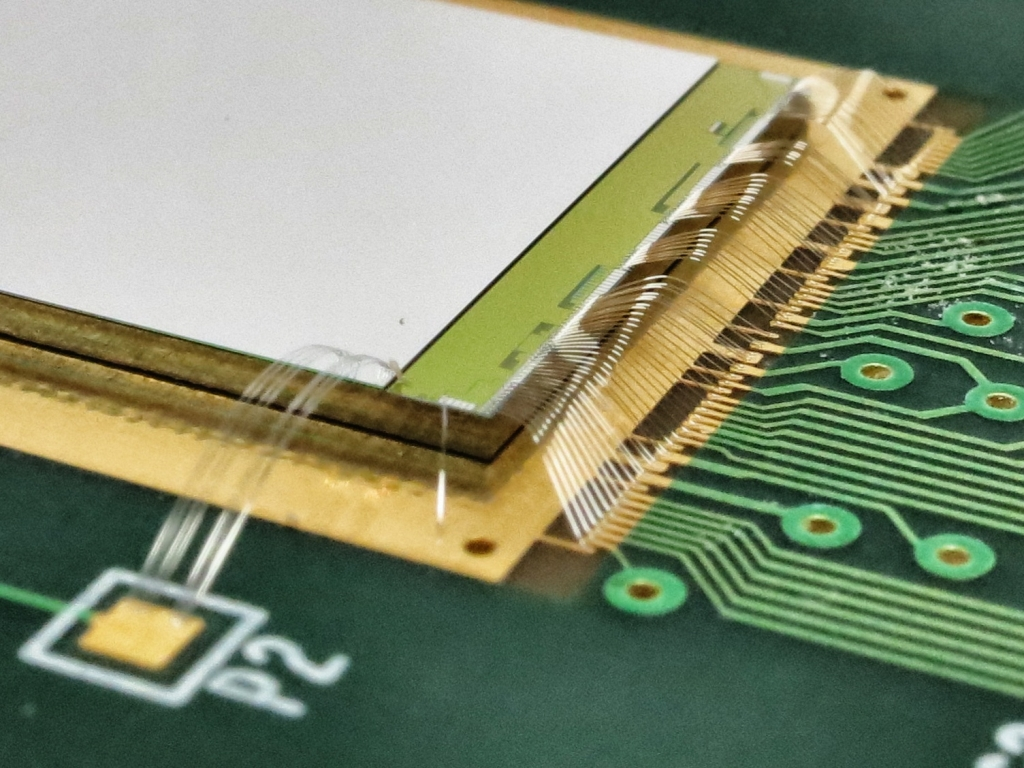
\includegraphics[width=0.9\textwidth]{figures/Advacam-50um-assembly.jpeg}
  \end{columns}

\end{frame}

\subsection{Setup for testing thin sensors}
\begin{frame}
  \frametitle{}
  \tableofcontents[currentsubsection]
\end{frame}
%%%%%%%%%%%%%%%%%%%%%%%%%%%%%
%         SLIDE             %
%%%%%%%%%%%%%%%%%%%%%%%%%%%%%
\begin{frame}
  \frametitle{Test-beam measurements of thin sensors}

  \begin{itemize}
  \item Test-beam campaigns at the CERN SPS (Super Proton Synchrotron)
    with $120\,\gev$ pion beam.
  \item CLICpix Timepix3 pixel-beam telescope
    \begin{itemize}
    \item 6 planes of Timepix3 hybrid detectors
    \item Track reconstruction.
    \end{itemize}
  \end{itemize}


  \begin{columns}

    \column{0.5\textwidth}
    
    \begin{itemize}
    \item Telescope pointing resolution
      \begin{itemize}
      \item \textcolor{Green}{$\sim2\,\micron$}
      \end{itemize}
    \item Hit resolution for the DUT
      \begin{itemize}
      \item Measured hit position on the DUT
        vs. reconstructed track.
      \end{itemize}
    % \item Time resolution per plane
    %   \begin{itemize}
    %   \item \textcolor{Green}{$\sim$1~ns}
    %   \end{itemize}
    \end{itemize}

    \column{0.5\textwidth}
    \centering
    \begin{tikzpicture}
      \node[anchor=south west,inner sep=0] (image) at
      (0,0){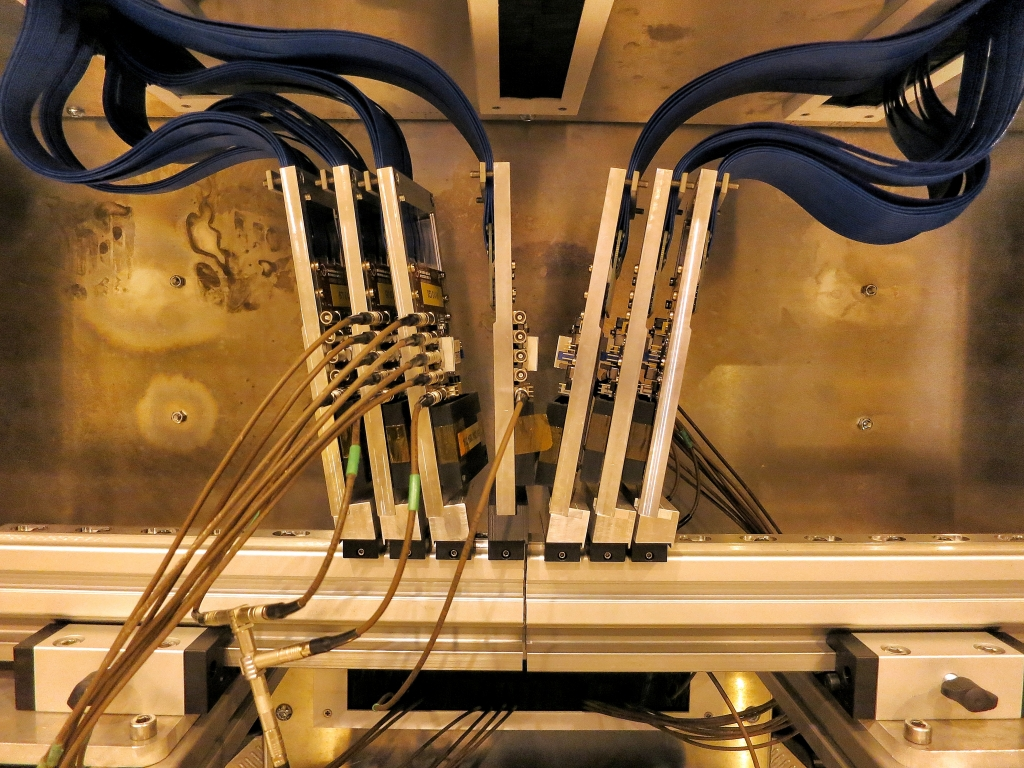
\includegraphics[width=\textwidth]{../figures/ActiveEdge/Timepix3Telescope.jpeg}};
      \begin{scope}[x={(image.south east)},y={(image.north west)}]
        \node[above, color=white] at (0.5, 0.85) {Device Under Test};
        \node[above, color=white] at (0.5, 0.75) {(\textbf{DUT})};

        \draw[->, very thick, color=black](0.75, 0.38) -- (0.25, 0.44);
        \draw[<->, very thick, color=Blue](0.33, 0.25) -- (0.66, 0.25);
        \node[below, color=Blue] at (0.5, 0.25) {\textbf{152~mm}};

        % \node[color=black] at (0.64, 0.32) {\textbf{0}};
        % \node[color=black] at (0.6, 0.32) {\textbf{1}};
        % \node[color=black] at (0.55, 0.32) {\textbf{2}};

        % \node[color=black] at (0.44, 0.32) {\textbf{3}};
        % \node[color=black] at (0.39, 0.32) {\textbf{4}};
        % \node[color=black] at (0.35, 0.32) {\textbf{5}};
        

        \node[circle, fill, color=Red, inner sep=0pt, minimum size=4pt]
        at (0.64, 0.4) {}; 
        \node[circle, fill, color=Red, inner sep=0pt, minimum size=4pt]
        at (0.6, 0.4) {};
        \node[circle, fill, color=Red, inner sep=0pt, minimum size=4pt]
        at (0.55, 0.4) {};
        \node[circle, fill, color=Red, inner sep=0pt, minimum size=4pt]
        at (0.42, 0.42) {};
        \node[circle, fill, color=Red, inner sep=0pt, minimum size=4pt]
        at (0.37, 0.43) {};
        \node[circle, fill, color=Red, inner sep=0pt, minimum size=4pt]
        at (0.32, 0.43) {};

        \node[star, fill, color=Green, inner sep=0pt, minimum size=8pt]
        at (0.49, 0.41) {};        
      \end{scope}
    \end{tikzpicture} 
    \\
    
    \begin{tikzpicture}
      \begin{scope}[x={(image.south east)},y={(image.north west)}]

        % \draw[help lines,xstep=.1,ystep=.1] (0, 0) grid (1,1);
        % \foreach \x in {0,1,...,9} { \node [anchor=north] at (\x/10,0) {0.\x}; }
        % \foreach \y in {0,1,...,9} { \node [anchor=east] at (0,\y/10) {0.\y}; }
        
         \node[circle, fill, color=Red, inner sep=0pt, minimum size=4pt]
        at (0.1, 0.9) {};
        \node[right, color=black] at (0.1, 0.9) {: measured track
          position};

        \node[star, fill, color=Green, inner sep=0pt, minimum
        size=8pt] at (0.1, 0.8) {}; \node[right, color=black] at (0.1,
        0.8) {: reconstructed track position};
      \end{scope}
    \end{tikzpicture} 



    % \begin{tikzpicture}
    %   \begin{scope}[x={(image.south east)},y={(image.north west)}]

    %     \draw[help lines,xstep=.1,ystep=.1] (0, 0) grid (1,1);
    %     \foreach \x in {0,1,...,9} { \node [anchor=north] at (\x/10,0) {0.\x}; }
    %     \foreach \y in {0,1,...,9} { \node [anchor=east] at (0,\y/10) {0.\y}; }
        
    %   \end{scope}
    % \end{tikzpicture} 

  \end{columns}

\end{frame}


\subsection{Simulation framework}
\begin{frame}
  \frametitle{}
  \tableofcontents[currentsubsection]
\end{frame}
%%%%%%%%%%%%%%%%%%%%%%%%%%%%%
%         SLIDE             %
%%%%%%%%%%%%%%%%%%%%%%%%%%%%%
\begin{frame}
  \frametitle{AllPix simulation framework}

  \begin{columns}
    \column{0.6\textwidth}

    \begin{itemize}
    \item A general purpose pixel-detector simulation framework (in
      C/C++) based on \textsc{Geant4}.
    \item Fully customisable for detector geometry description:
      \begin{itemize}
      \item thickness, pixel-pitch, bump geometry, material
      \end{itemize}
    \item \textcolor{Green}{\textbf{Digitisation}}: responsible for the
      full simulation of the detector including the sensor and the
      readout chip. 
      \begin{itemize}
      \item Defined by the user.
      \item Different for each sensor/ASIC technology.
      \end{itemize}
    \end{itemize}
    
    \column{0.4\textwidth}
    \centering
    \begin{tikzpicture}
      \node[anchor=south west,inner sep=0] (image) at
      (0,0){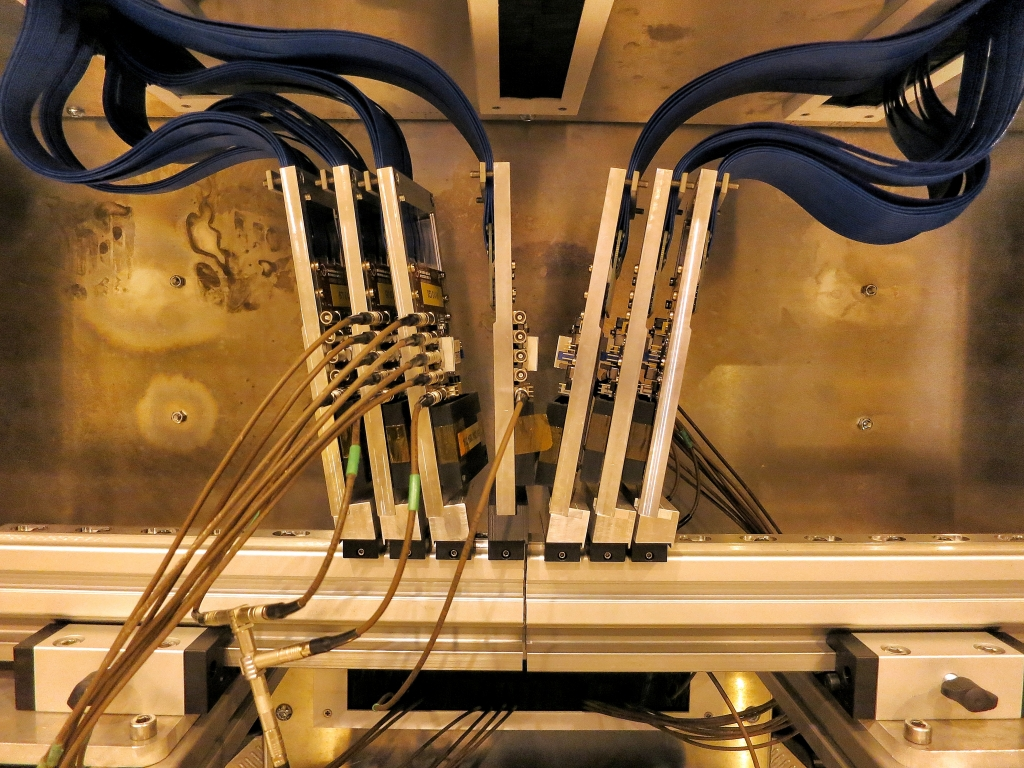
\includegraphics[width=\textwidth]{../figures/ActiveEdge/Timepix3Telescope.jpeg}};
      \begin{scope}[x={(image.south east)},y={(image.north west)}]
        \node[above, color=white] at (0.5, 0.85) {The telescope};
      \end{scope}
    \end{tikzpicture}

    \centering
    \begin{tikzpicture}
      \node[anchor=south west,inner sep=0] (image) at
      (0,0){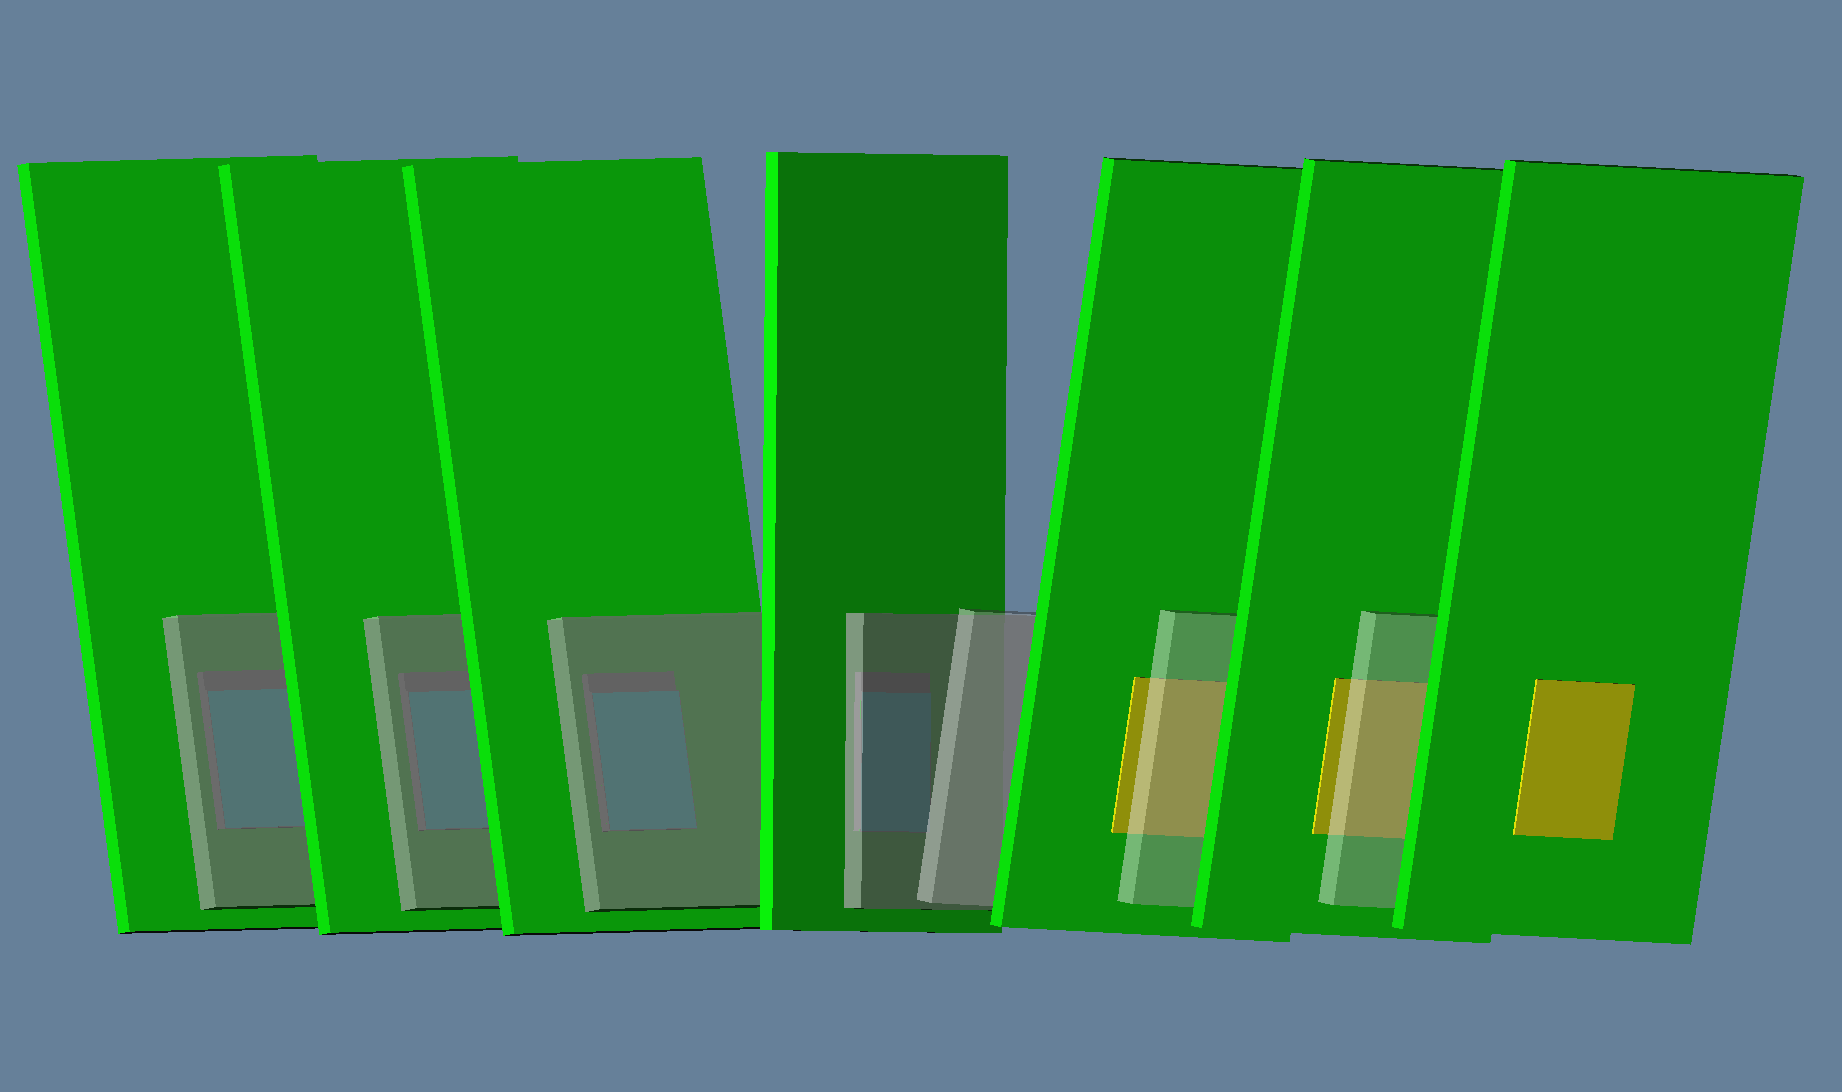
\includegraphics[width=\textwidth]{../figures/Telescope/AllpixTelescope.png}};

      \begin{scope}[x={(image.south east)},y={(image.north west)}]
        \node[above, color=white] at (0.5, 0.8) {The simulated telescope};
      \end{scope}
    \end{tikzpicture}
  \end{columns}

  \begin{itemize}
  \item \textcolor{Red}{Goal}:
    \begin{itemize}
    \item Simulate the test-beam setup.
    % \item Extrapolate results for small-pitch pixels (e.g.  CLICpix
    %   with $25\,\micron$ pitch).
    \item Improve digitisation models for full-detector simulation.
    \end{itemize}
  \end{itemize}

\end{frame}

\subsection{The telescope performance}
\begin{frame}
  \frametitle{}
  \tableofcontents[currentsubsection]
\end{frame}
%%%%%%%%%%%%%%%%%%%%%%%%%%%%%
%         SLIDE             %
%%%%%%%%%%%%%%%%%%%%%%%%%%%%%
\begin{frame}
  \frametitle{The Timepix3 telescope performance}

  \begin{itemize}
  \item In simulation, extract the telescope pointing resolution on
    the DUT using the Monte Carlo (MC) hit position
  \end{itemize}

  \begin{columns}
    \column{0.5\textwidth}
    \begin{itemize}
    \item Biased residual: reconstructed track vs. measured hit on the
      telescope planes.
    \item Agreement between data and simulation \ding{51}
    \end{itemize}

    \column{0.5\textwidth}
    \centering
    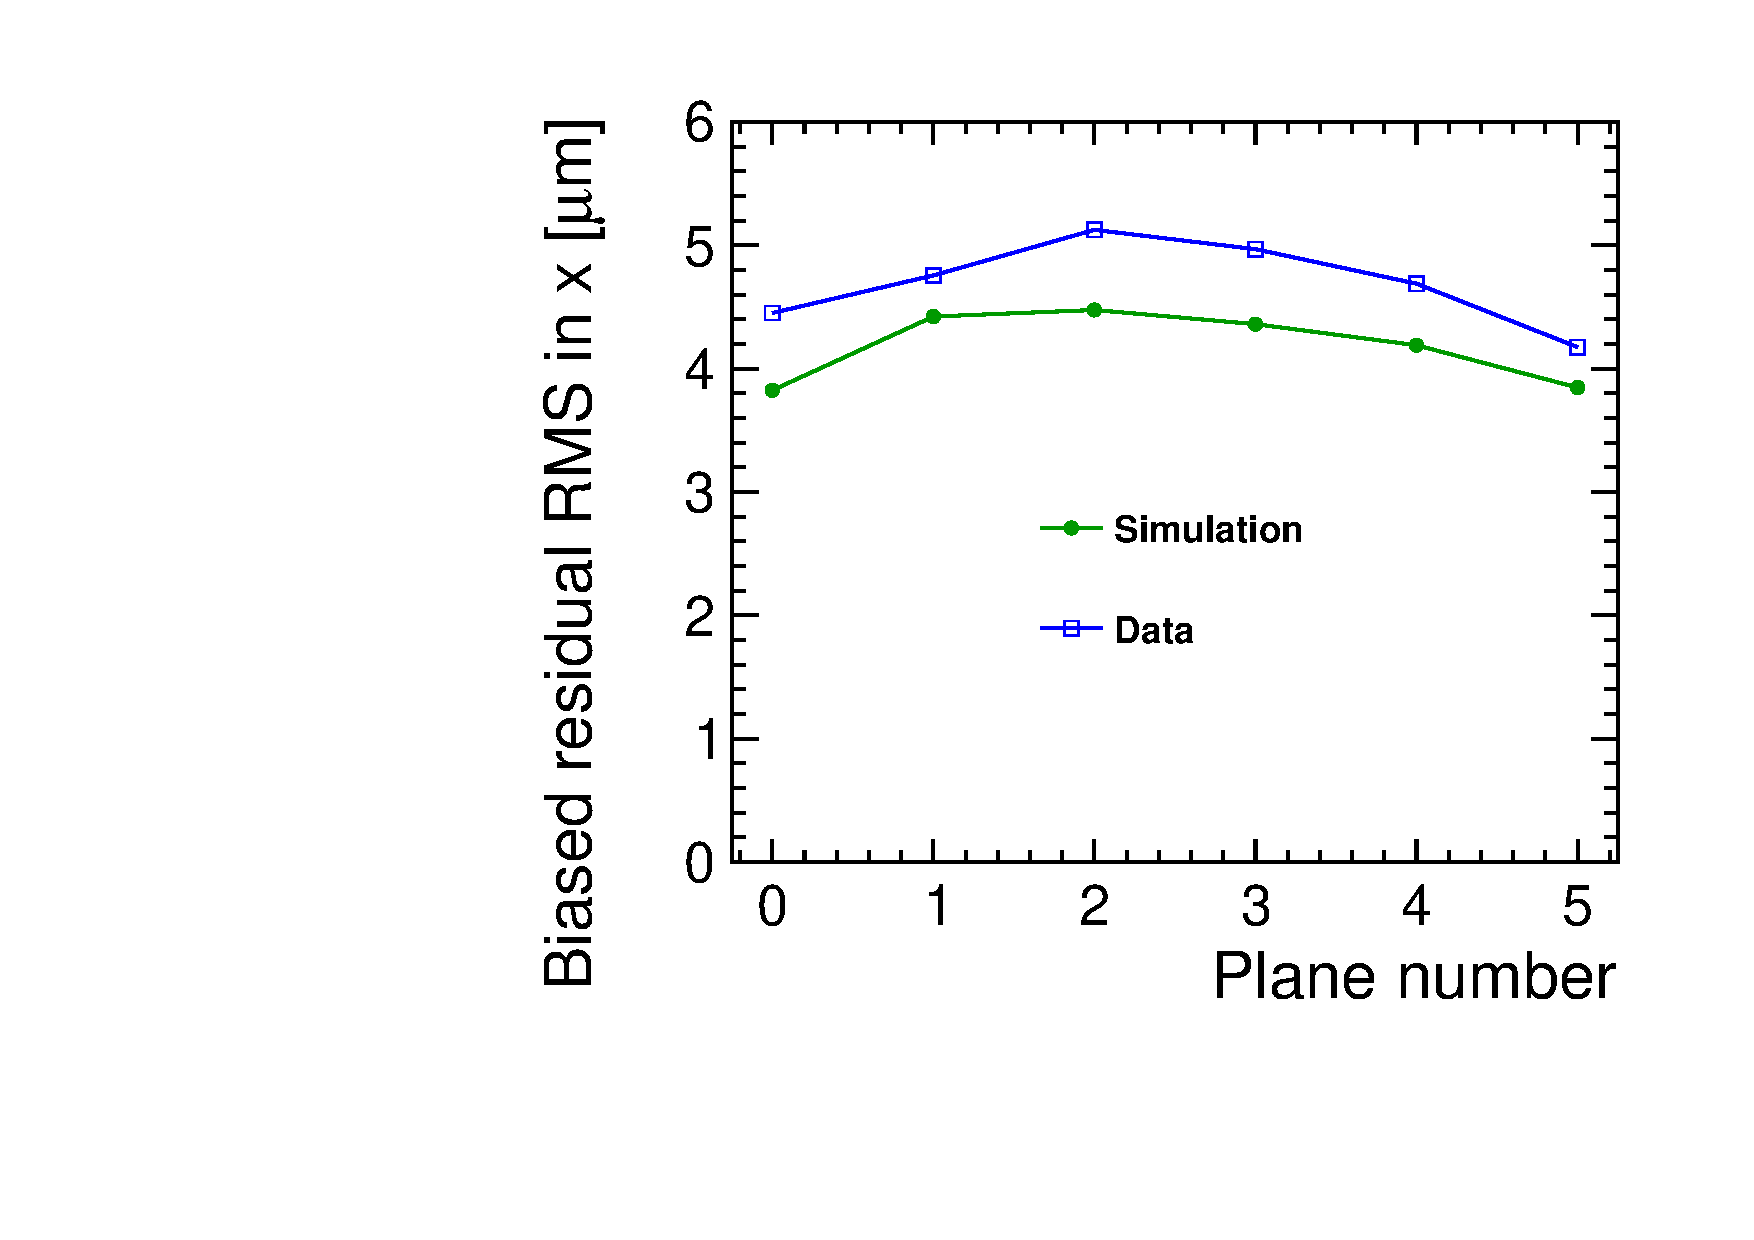
\includegraphics[width=0.8\textwidth]{../figures/Telescope/biasedResiduals/RMSX_simu_vs_data.pdf}
  \end{columns}

  \begin{columns}
    \column{0.5\textwidth}
    \begin{itemize}
    \item Tracking resolution on the DUT: reconstructed track vs. MC
      hit position
    \item Excellent tracking resolution of
      \textcolor{Green}{$\sim2\,\micron$} on the DUT
      \\
      $\Rightarrow$ In agreement with the expectations \ding{51}
    \end{itemize}

    \column{0.5\textwidth}
    \centering
    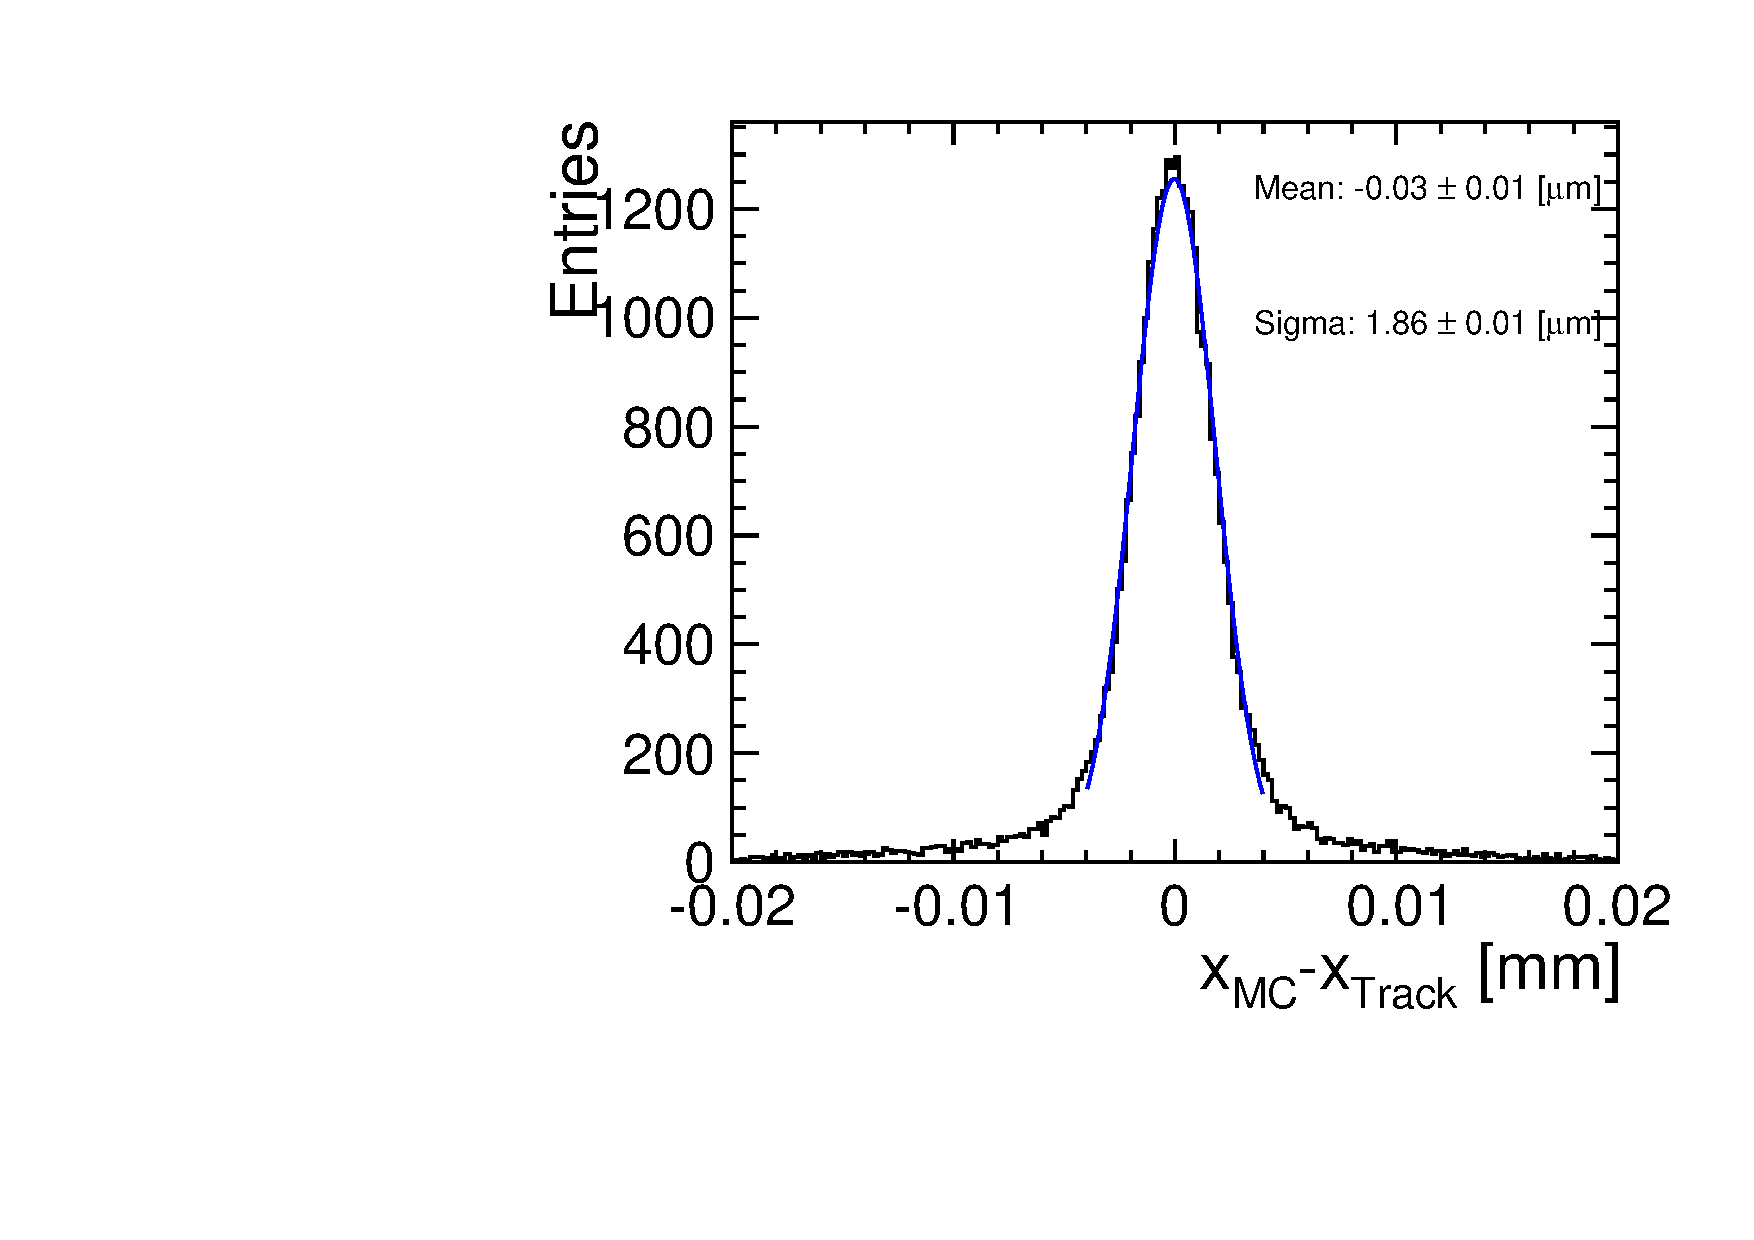
\includegraphics[width=0.8\textwidth]{../figures/Telescope/Unbiased_trackRes_DUT_x.pdf}
  \end{columns}

\end{frame}


\subsection{The performance of thin sensors}
\begin{frame}
  \frametitle{}
  \tableofcontents[currentsubsection]
\end{frame}
%%%%%%%%%%%%%%%%%%%%%%%%%%%%%
%         SLIDE             %
%%%%%%%%%%%%%%%%%%%%%%%%%%%%%
{
  \usebackgroundtemplate{
    \begin{picture}(0, 270)
      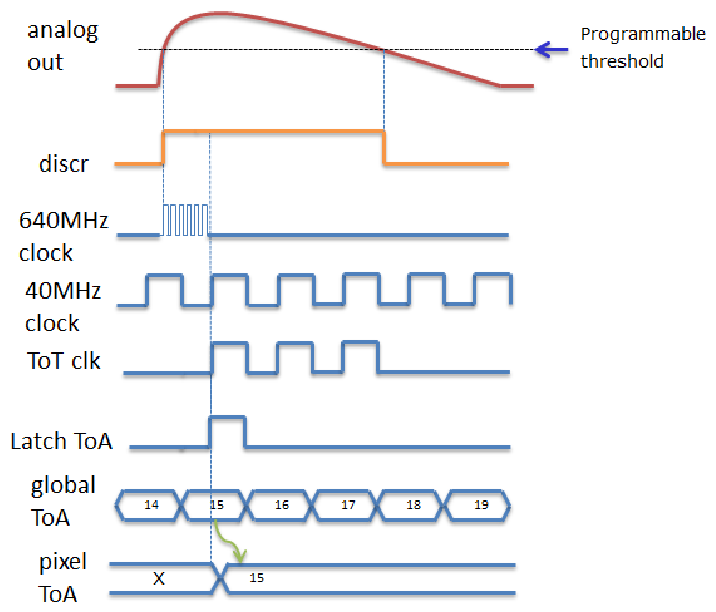
\includegraphics[width=0.6\textwidth]{figures/TOT_TOA_explanation.pdf}
    \end{picture}
  }%
  \begin{frame}
    \frametitle{The Timepix3 readout chip}

    \begin{itemize}
    \item Test vehicle for thin sensors: \textcolor{Green}{sensor} \&
      \textcolor{blue}{Timepix3 readout ASIC}
    \end{itemize}

    \centering
    \begin{adjustbox}{max totalsize={1.1\textwidth}{.7\textheight},center}
      \begin{tikzpicture}[node distance = 2.5cm, auto]
        \begin{scope}[x={(image.south east)},y={(image.north west)}]
          
          \coordinate (input);
          \node [block, right of=input, color=Green] (sens) {Sensor};
          \node [block, right of=sens, color=blue] (preamp) {Preamplifier/ Shaper};
          \node [block, right of=preamp, color=blue] (discr) {Discriminator};
          \node [block, right of=discr, color=blue] (conv) {TOT/TOA counters};
          \coordinate[right of=conv] (output);
          
          \draw[arrows=->] (input) -- node [text
          width=4cm,midway] {Incident radiation} (sens);
          \draw[arrows=->] (sens) -- (preamp);
          \draw[arrows=->] (preamp) -- (discr);
          \draw[arrows=->] (discr) -- (conv);
          \draw[arrows=->] (conv) -- node [text width=1.5cm,midway]
          {Digital data bus} (output);
          
          \draw[decorate,decoration={brace, mirror}, thick] (sens.south) to
          node[below,below] (bracket) {Analogue domain}
          (discr.south);
          
          \draw[decorate,decoration={brace, mirror}, thick] (conv.south
          west) to node[below,below] (bracket) {Digital domain} (conv.south
          east);
          
          \draw[decorate,decoration={brace}, thick, color=blue] (preamp.north) to
          node[above, above] (bracket) {Readout chip} (conv.north);
        \end{scope}
      \end{tikzpicture}
    \end{adjustbox}


    \vspace{-0.2cm}
    \begin{columns}
      \column{0.5\textwidth}
      \column{0.5\textwidth}
      \begin{itemize}
      \item Matrix of $256\times256$ pixels
      \item $55\,\micron$ pixel pitch (130~nm CMOS technology)
      \item Simultaneous measurement:
        \begin{itemize}
        \item Time-over-threshold (TOT), 10 bit $\Rightarrow$
          \textcolor{Green}{energy}
        \item Time-of-arrival (TOA), 18 bit $\Rightarrow$
          \textcolor{Green}{time}
        \end{itemize}
      % \item Data-driven mode readout:
      %   \begin{itemize}
      %   \item Low dead time
      %   \item High readout rates%: 40~Mhits/(s$\cdot$cm\textsuperscript{2})
      %   \end{itemize}
      \item Electronic noise: $\sim80$~e\textsuperscript{-} RMS
        \begin{itemize}
        \item Operating threshold: $\sim500$~e\textsuperscript{-}
        \end{itemize}
      \end{itemize}
    \end{columns}
  \end{frame}
}

%%%%%%%%%%%%%%%%%%%%%%%%%%%%%
%         SLIDE             %
%%%%%%%%%%%%%%%%%%%%%%%%%%%%%
\begin{frame}
  \frametitle{Energy deposition in thin sensors}

  \begin{columns}
    \column{0.6\textwidth}
    \begin{itemize}
    \item Energy deposition (E\textsubscript{dep}) in silicon sensors is
      subject to statistical fluctuations
    \item Chip calibration (internal test-pulse generation): parametrise
      the relationship between the TOT measurement and the E\textsubscript{dep}
    \end{itemize}

    \column{0.4\textwidth}
    \centering
    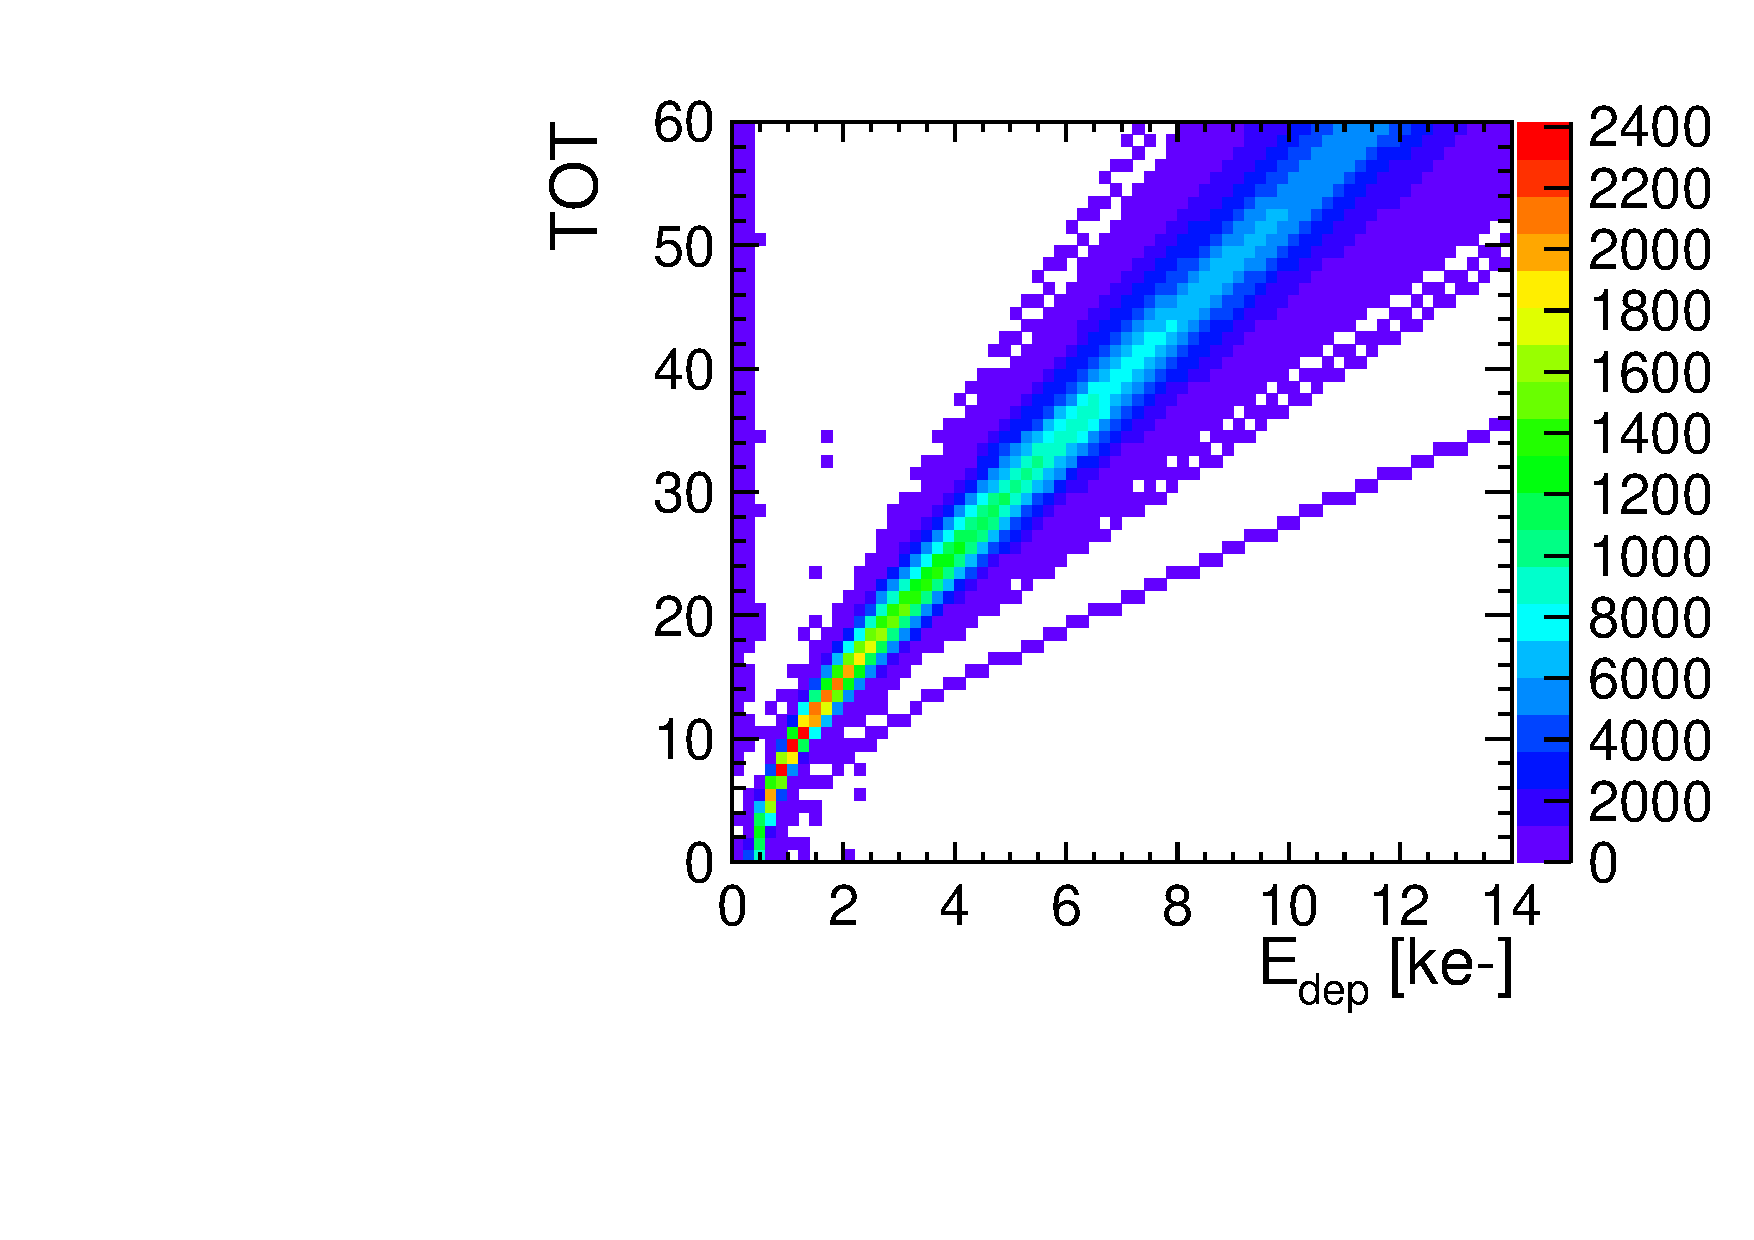
\includegraphics[width=\textwidth]{../figures/Calibration/TOTcalibration_W0005_E02_thresh1160.pdf}
  \end{columns}

  \begin{itemize}
  \item Good agreement between data and simulation \ding{51}
  \end{itemize}


  \begin{columns}
    \column{0.33\textwidth}
    \begin{itemize}
    \item $50\,\micron$
    \end{itemize}
    \centering
    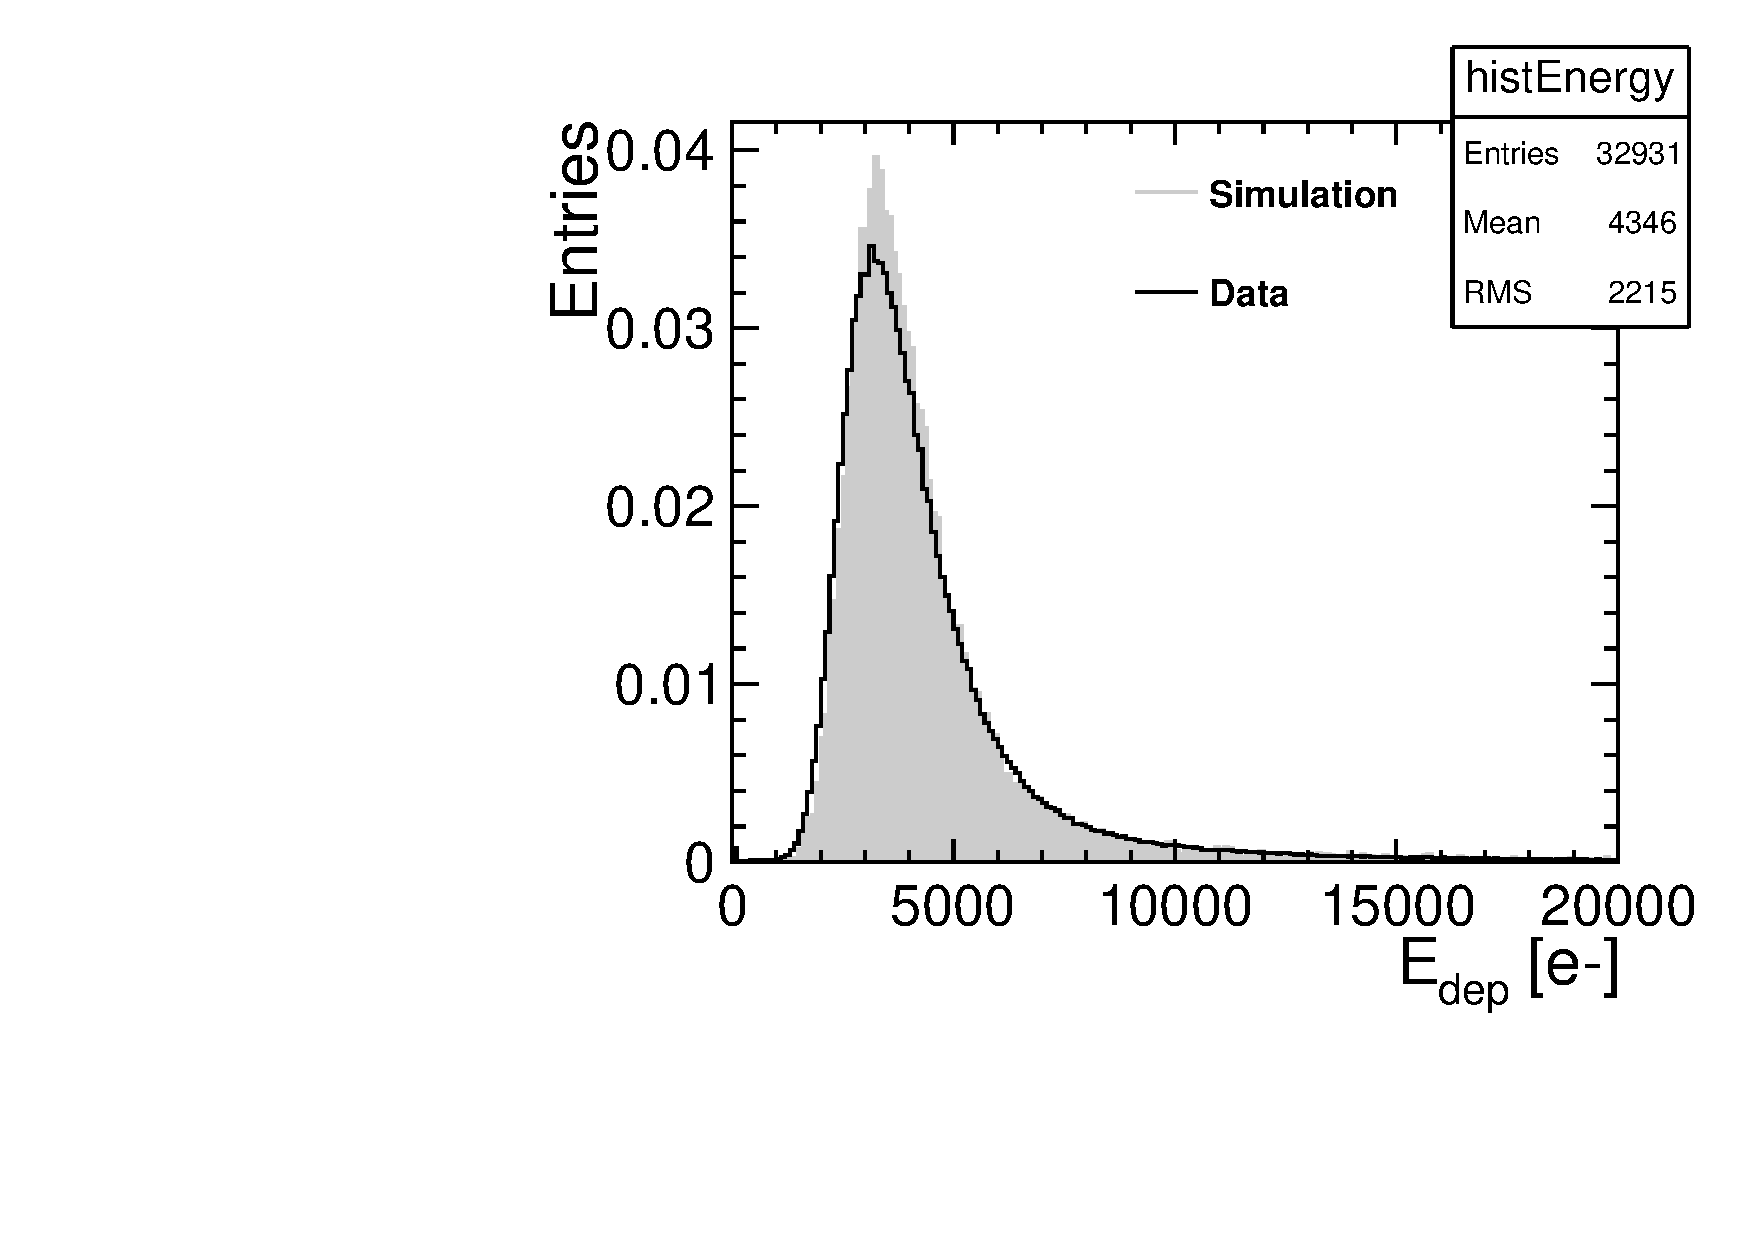
\includegraphics[width=\textwidth]{../figures/TestBeam/50micron_Edep.pdf}

    \column{0.33\textwidth}
    \begin{itemize}
    \item $100\,\micron$
    \end{itemize}
    \centering
    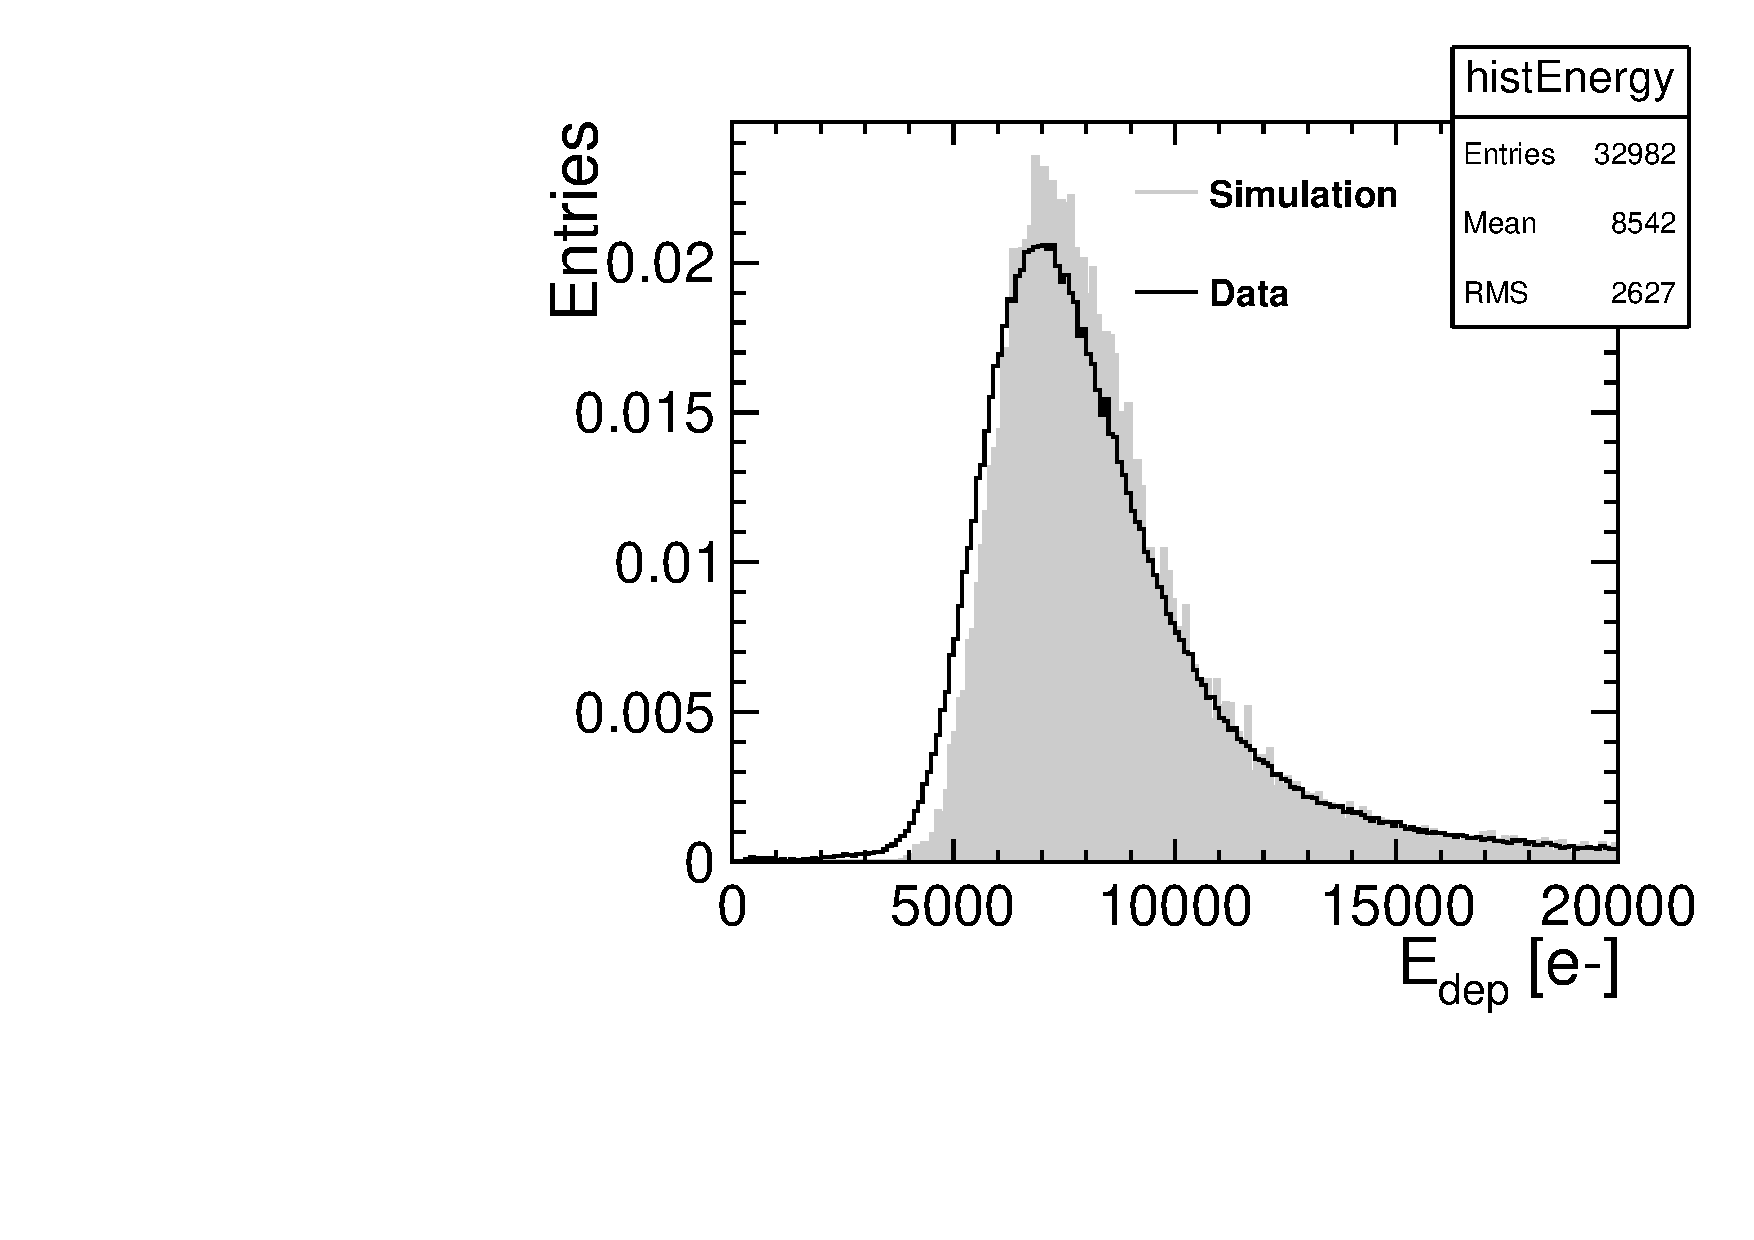
\includegraphics[width=\textwidth]{../figures/TestBeam/100micron_Edep.pdf}

    \column{0.33\textwidth}
    \begin{itemize}
    \item $150\,\micron$
    \end{itemize}
    \centering
    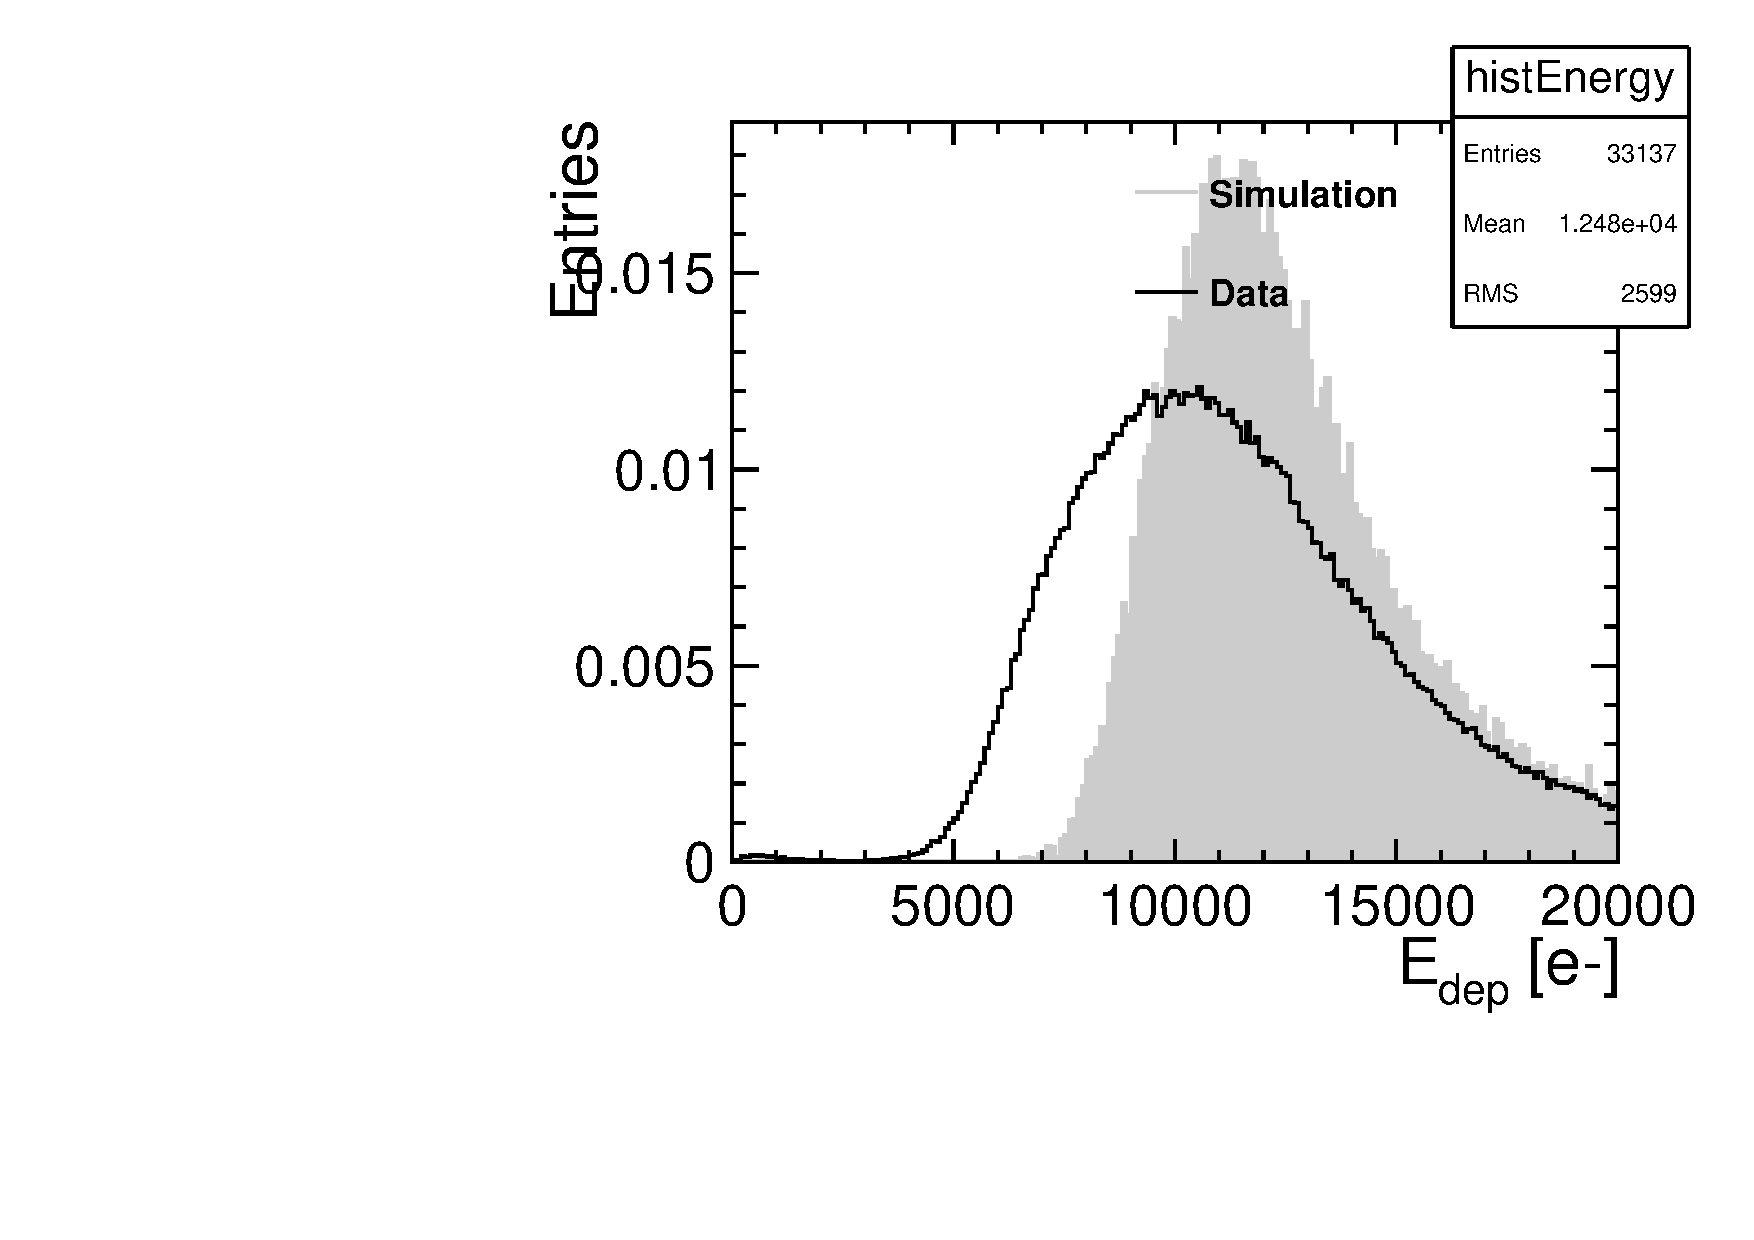
\includegraphics[width=\textwidth]{../figures/TestBeam/150micron_Edep.pdf}
  \end{columns}

\end{frame}

%%%%%%%%%%%%%%%%%%%%%%%%%%%%%
%         SLIDE             %
%%%%%%%%%%%%%%%%%%%%%%%%%%%%%
\begin{frame}
  \frametitle{Charge sharing}

  \begin{itemize}
  % \item Spread of the charge carriers at the readout due to their
  %   diffusion within the detector volume.
  % \item Cluster-size distribution $\Rightarrow$ indication of charge
  %   sharing.
  \item Cluster size vs. track position within pixel:
  \end{itemize}

  \vspace{-0.5cm}

  \begin{columns}[t]
    \column{0.25\textwidth}
    \begin{itemize}
    \item 1-pixel
    \end{itemize}
    \begin{tikzpicture}
      \draw (0,0) rectangle (0.5,-0.5);
    \end{tikzpicture}
    \centering

    \vspace{0.5cm}

    \begin{tikzpicture}
      \node[anchor=south west,inner sep=0] (image) at
      (0,0){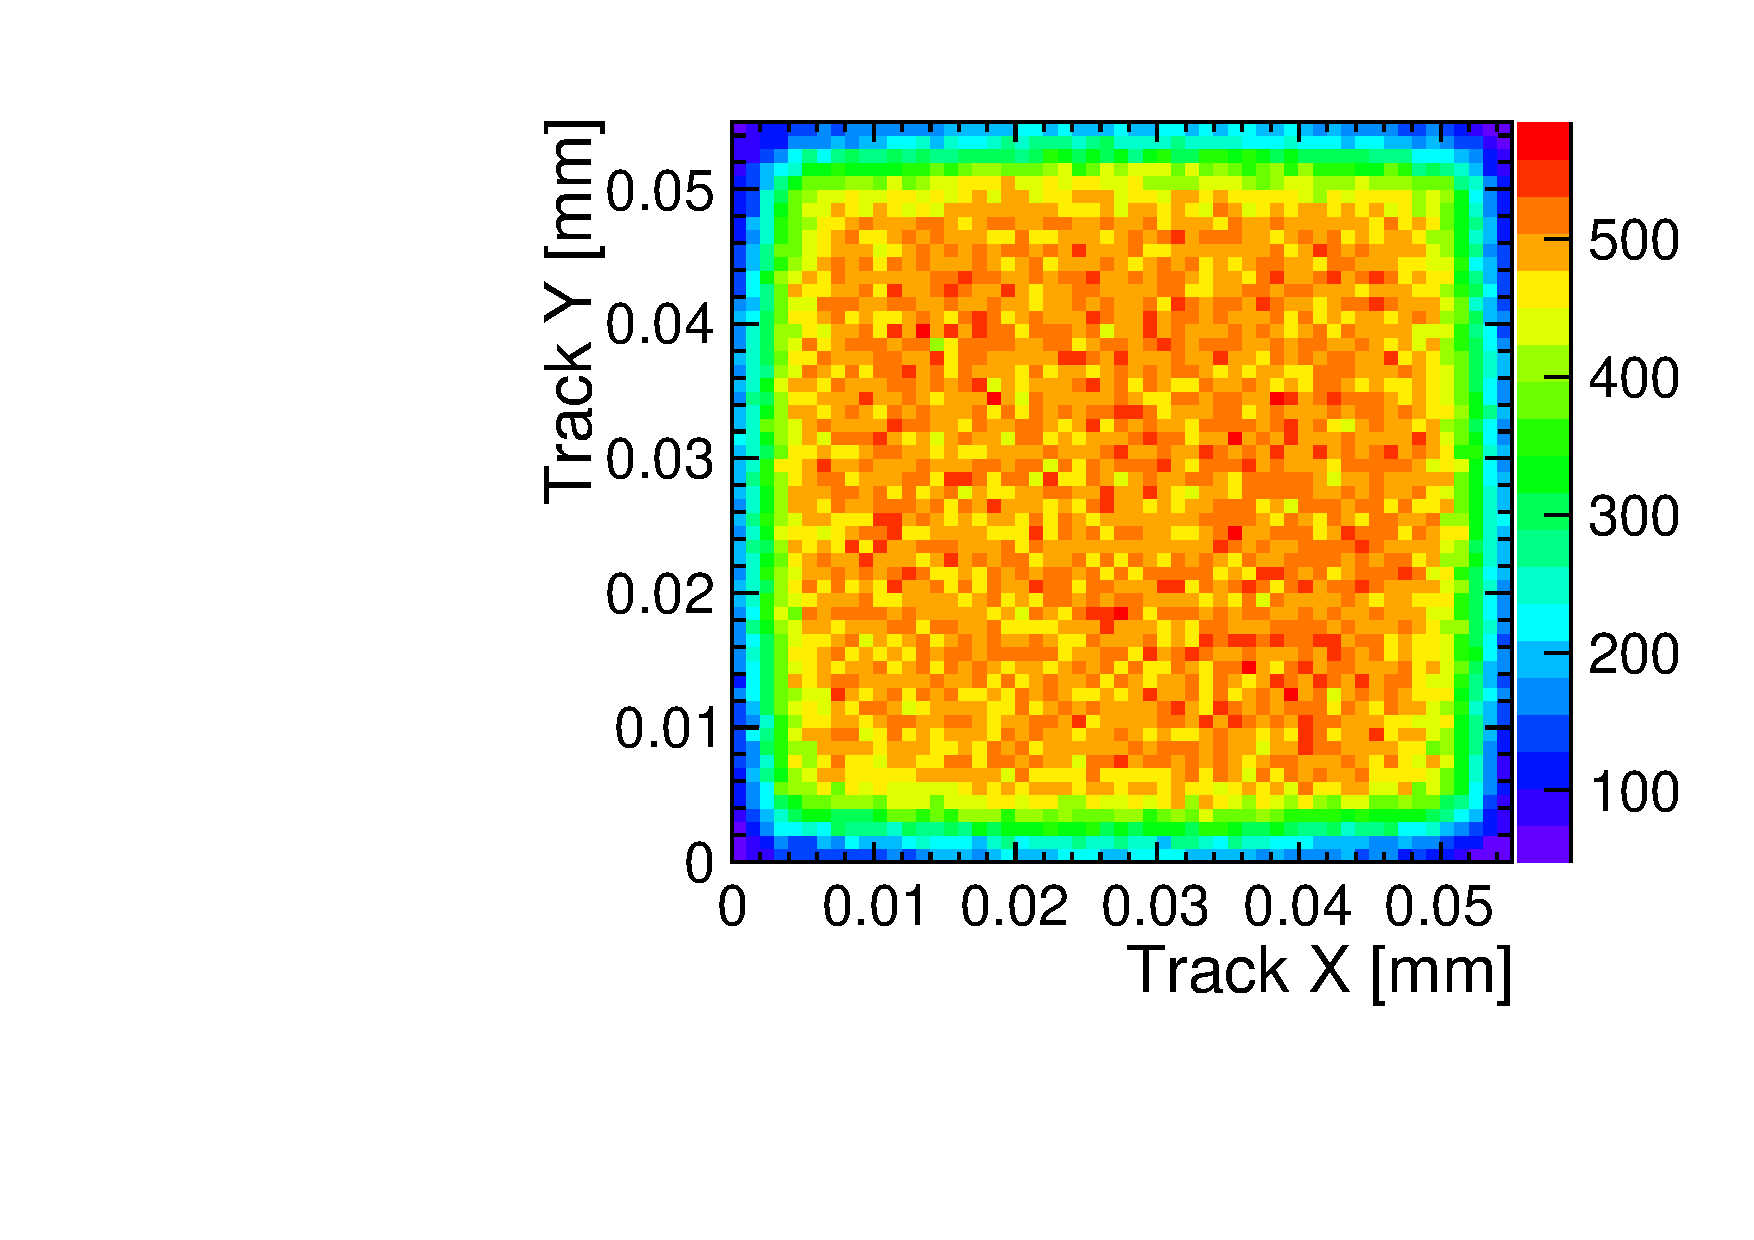
\includegraphics[width=\textwidth]{../figures/TestBeam/TrackPosWPixel_1hit_runW19_G7.pdf}};
      \begin{scope}[x={(image.south east)},y={(image.north west)}]

        \draw[<->, very thick, color=Blue](0.18, 0) -- (0.82, 0);
        \node[below, color=Blue] at (0.5, 0.0) {pitch};
      \end{scope}
    \end{tikzpicture}
    

    \column{0.25\textwidth}
    \begin{itemize}
    \item 2-pixel
    \end{itemize}
    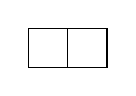
\begin{tikzpicture}
      \draw (0.0,0.0) rectangle (0.5,-0.5);
      \draw (0.5,0.0) rectangle (1.0,-0.5);
    \end{tikzpicture}
    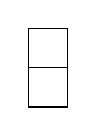
\begin{tikzpicture}
      \draw (0.0,0.0) rectangle (0.5,-0.5);
      \draw (0.0,0.5) rectangle (0.5,0.0);
    \end{tikzpicture}
    \centering
    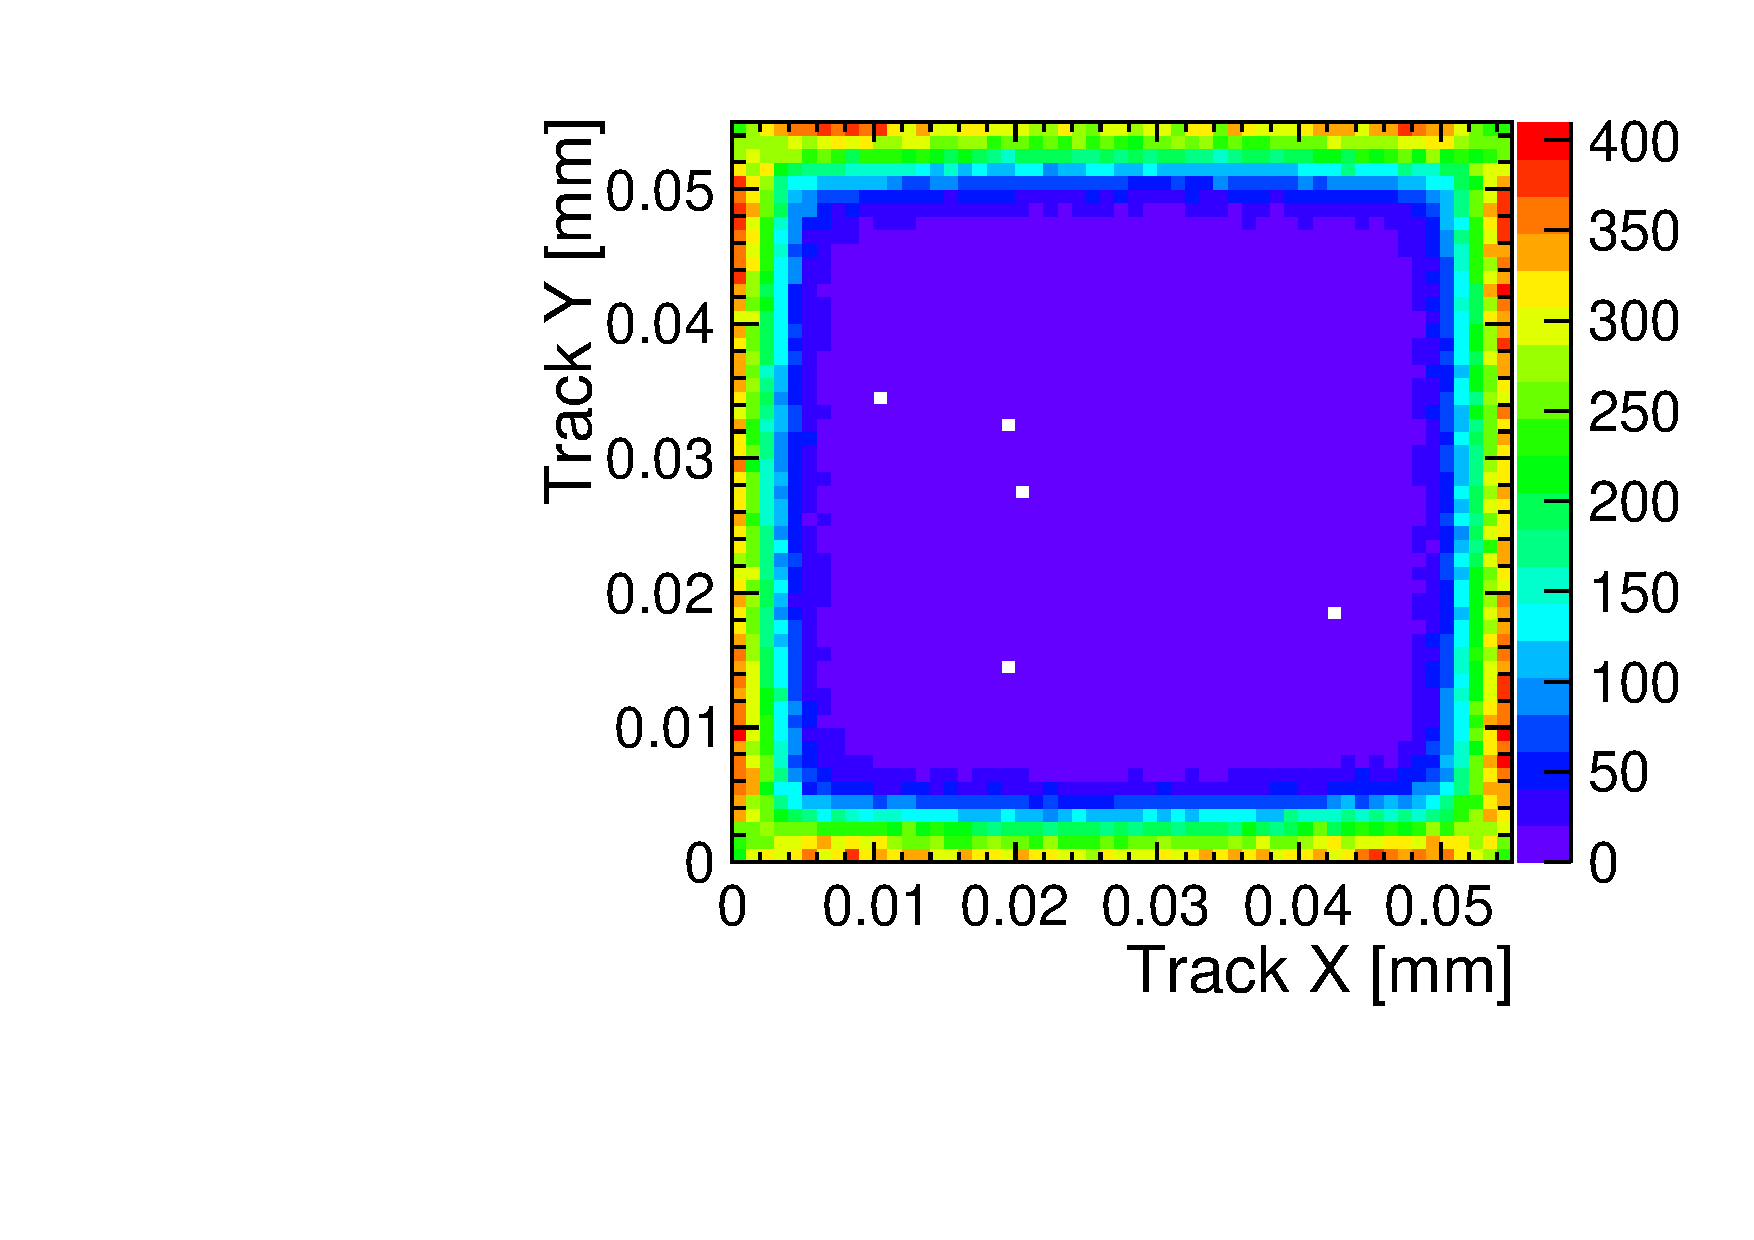
\includegraphics[width=\textwidth]{../figures/TestBeam/TrackPosWPixel_2hit_runW19_G7.pdf}

    \column{0.25\textwidth}
    \begin{itemize}
    \item 3-pixel
    \end{itemize}
    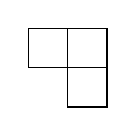
\begin{tikzpicture}
      \draw (0.0,0.0) rectangle (0.5,-0.5);
      \draw (0.5,-0.5) rectangle (1.0,-1.0);
      \draw (0.5,0.0) rectangle (1.0,-0.5);
    \end{tikzpicture}
    \centering
    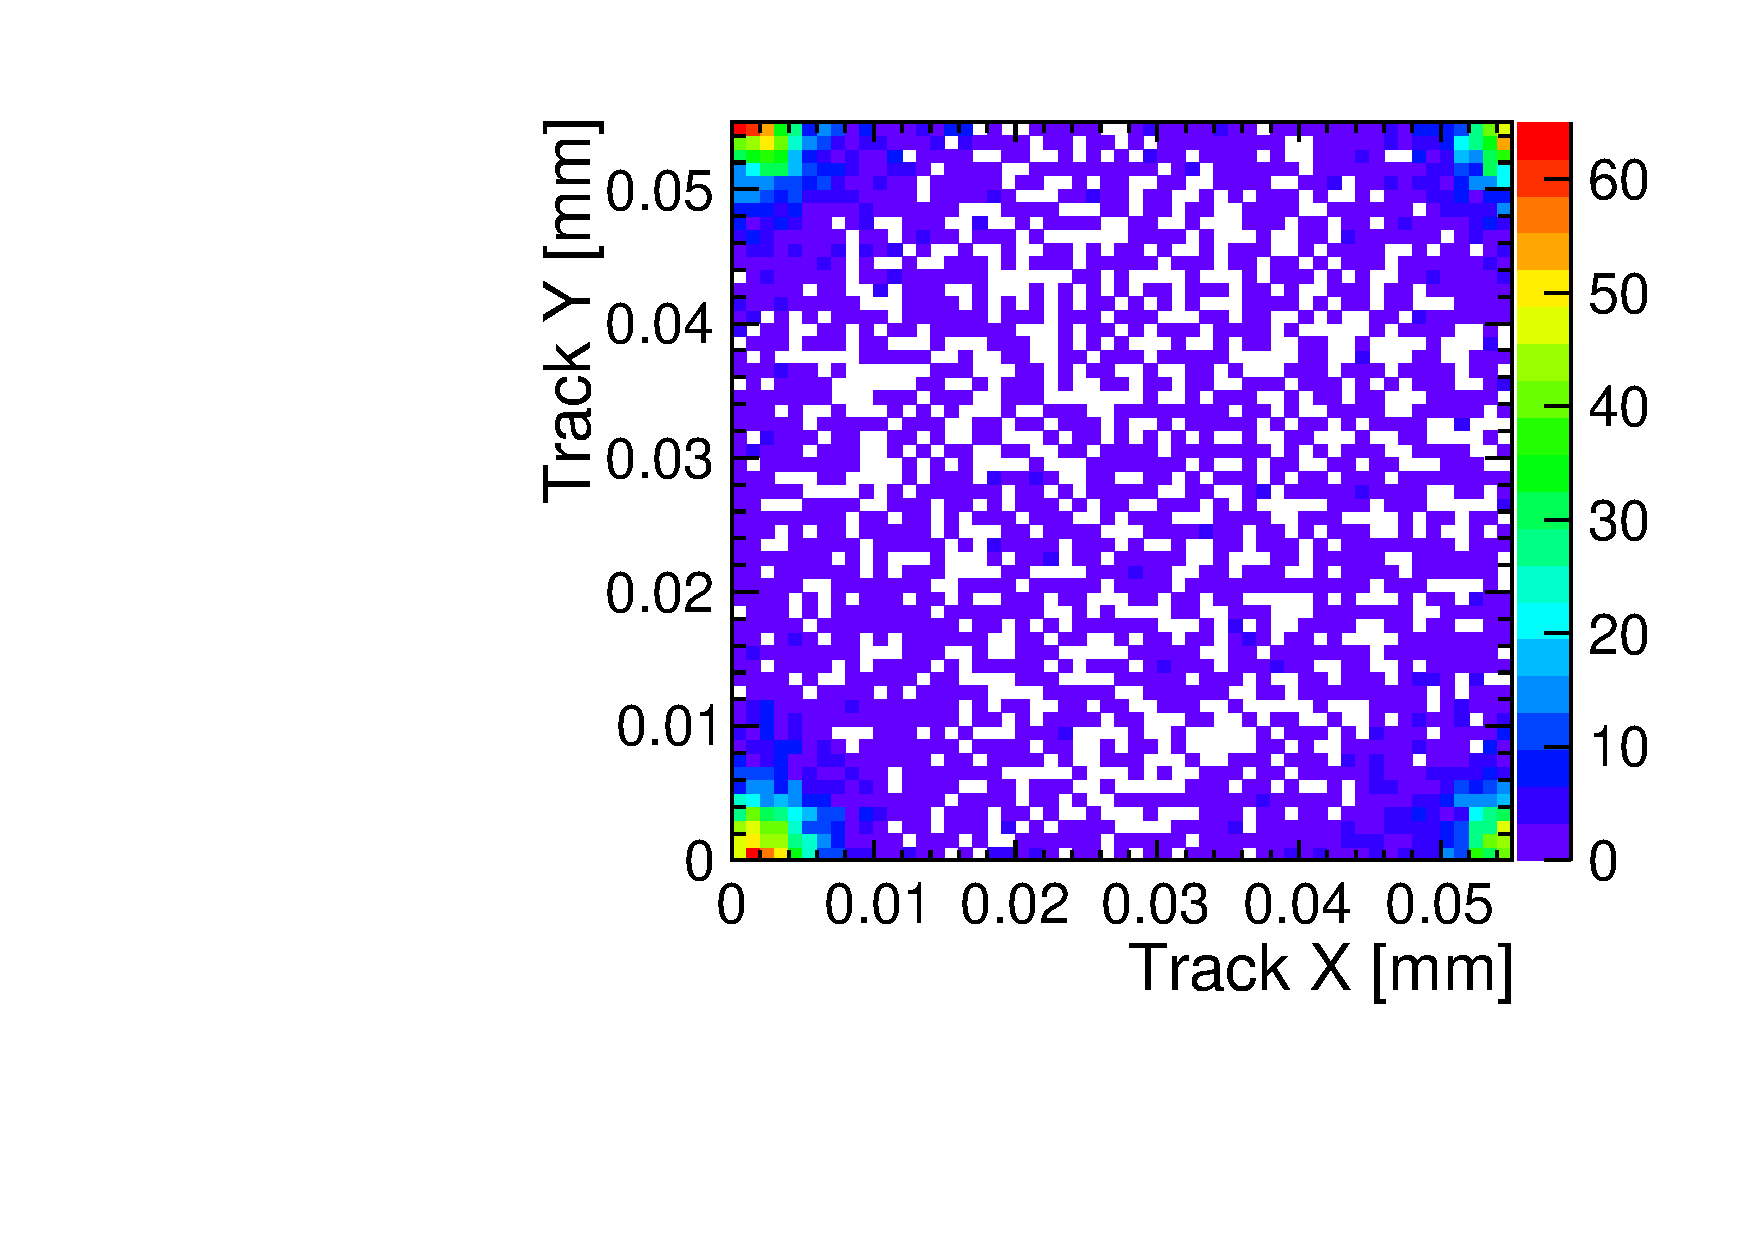
\includegraphics[width=\textwidth]{../figures/TestBeam/TrackPosWPixel_3hit_runW19_G7.pdf}

    \column{0.25\textwidth}
    \begin{itemize}
    \item 4-pixel
    \end{itemize}
    
\begin{tikzpicture}
      \draw (0.0,0.0) rectangle (0.5,-0.5);
      \draw (0.5,-0.5) rectangle (1.0,-1.0);
      \draw (0.5,0.0) rectangle (1.0,-0.5);
      \draw (0.0,-0.5) rectangle (0.5,-1.0);
    \end{tikzpicture}
    \centering
    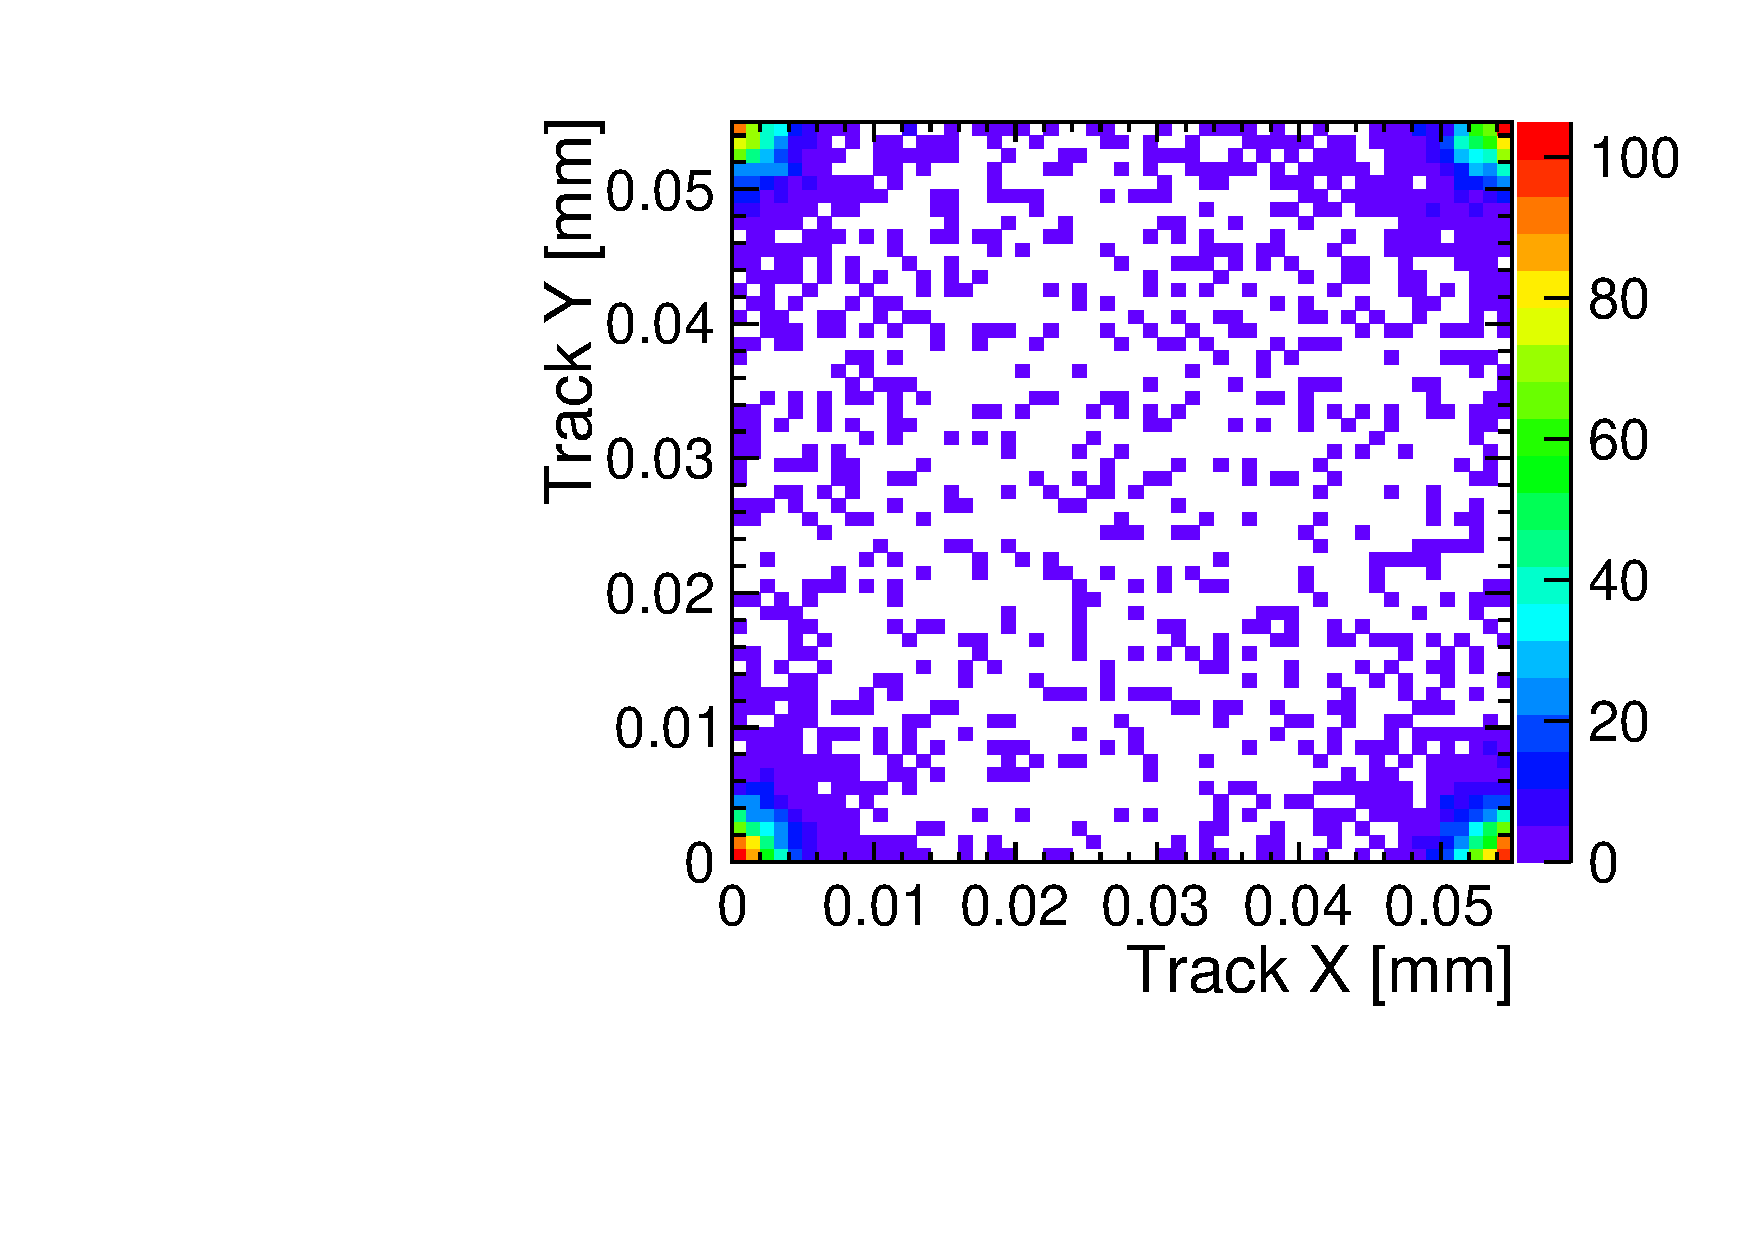
\includegraphics[width=\textwidth]{../figures/TestBeam/TrackPosWPixel_4hit_runW19_G7.pdf}
  \end{columns}

  \vspace{-0.5cm}
  \begin{columns}
    \column{0.5\textwidth}
    \begin{itemize}
    \item Factors affecting the charge sharing:
      \begin{itemize}
      \item Sensor thickness
      \item Bias voltage
      \item Readout threshold 
      \end{itemize}
    \end{itemize}

    $\Rightarrow$ Good agreement between data and simulation

    \column{0.5\textwidth}
    \centering
    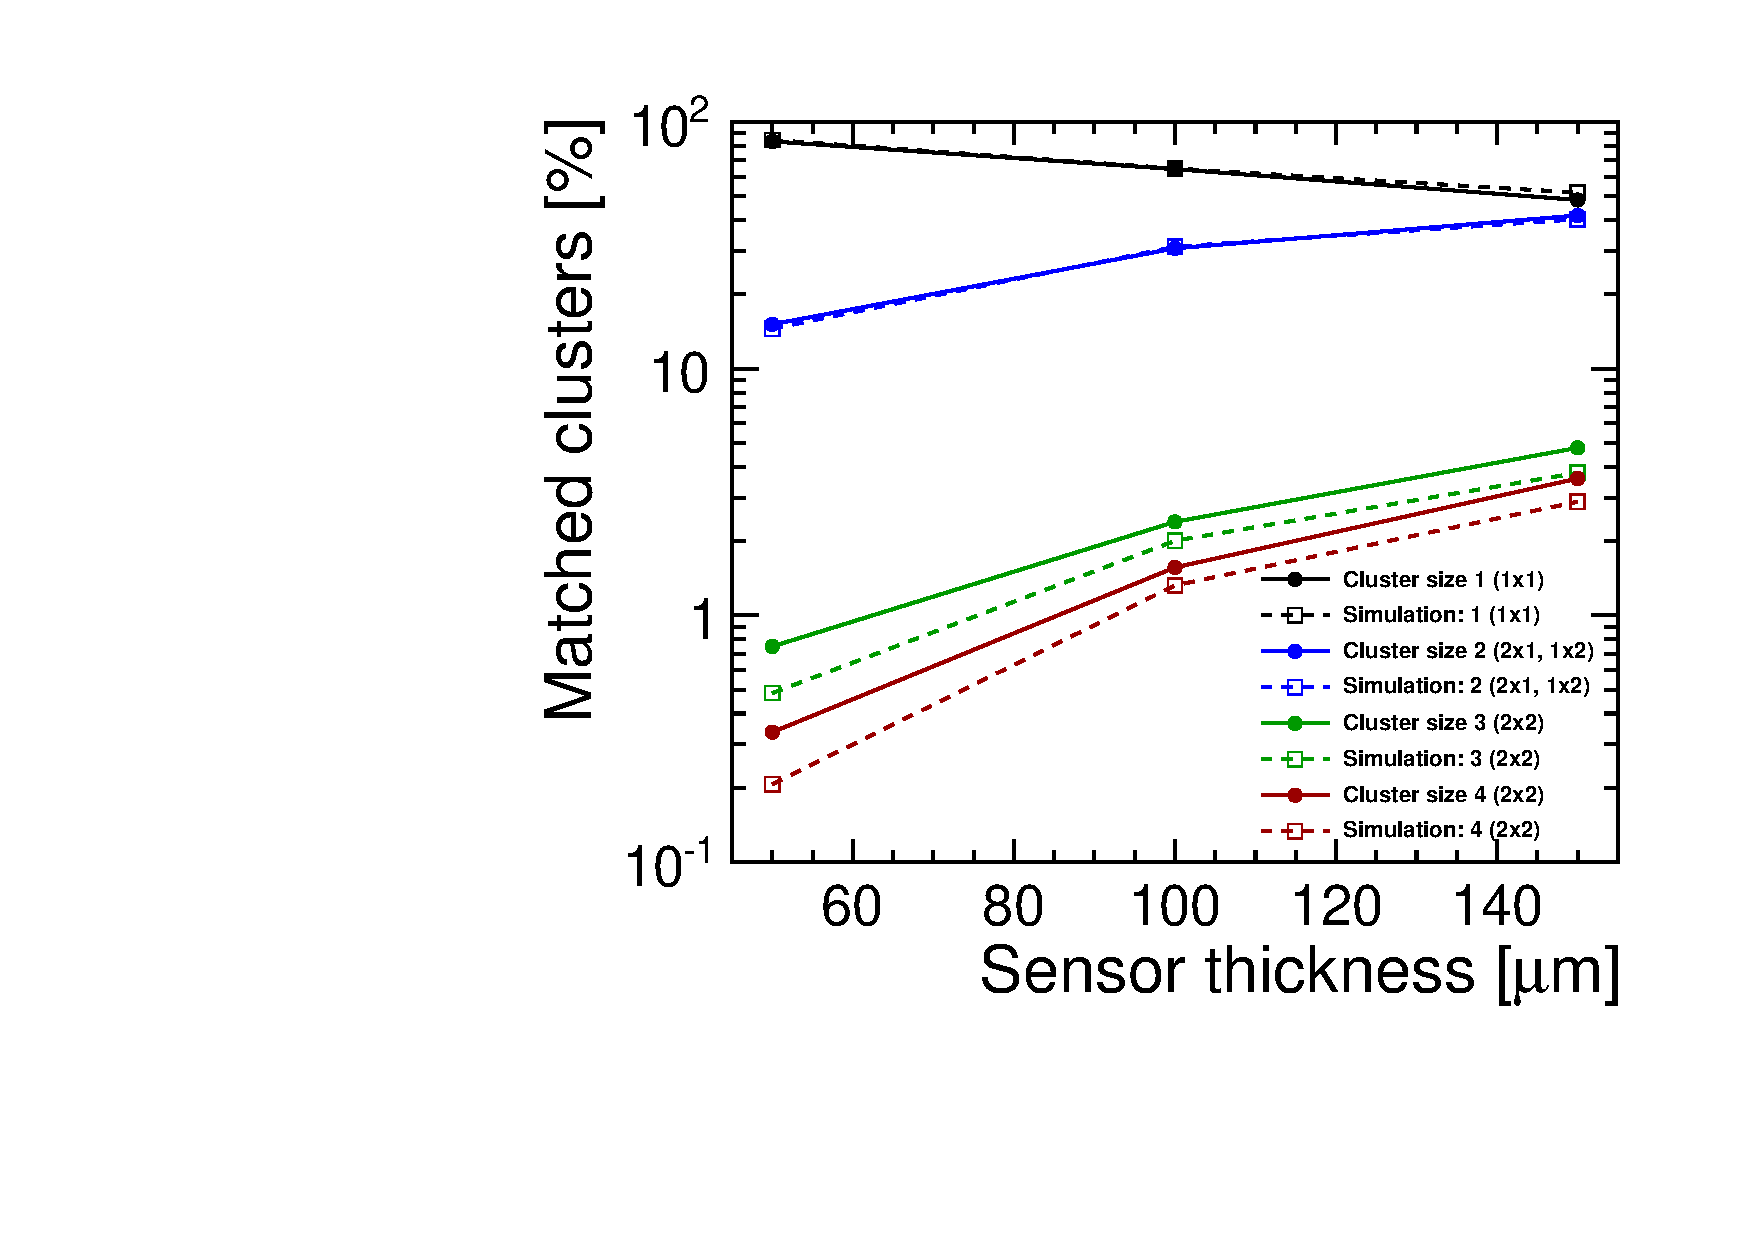
\includegraphics[width=0.8\textwidth]{../figures/TestBeam/cluSize_vs_thickness.pdf}
  \end{columns}

\end{frame}

%%%%%%%%%%%%%%%%%%%%%%%%%%%%%
%         SLIDE             %
%%%%%%%%%%%%%%%%%%%%%%%%%%%%%
\begin{frame}
  \frametitle{Hit resolution}

  \begin{columns}[t]
    \column{0.5\textwidth}
    \begin{itemize}
    \item Hit resolution considering only geometrical information\\
      \begin{equation*}
        \sigma={\text{pitch} \over \sqrt{12}}
      \end{equation*}
    \item The overall resolution depends on the cluster-size
      distribution
      \begin{itemize}
      \item \textcolor{Green}{Single-pixel clusters}: hit
        reconstructed at the geometric center of the pixel
      \item \textcolor{Green}{Multi-pixel clusters}: the
        reconstruction takes into account the non-linearity of charge
        sharing for the hit reconstruction.
      \end{itemize}
    \end{itemize}

    \column{0.5\textwidth}
    \begin{itemize}
    \item For $150\,\micron$ sensor
    \end{itemize}

    \centering
    \begin{tikzpicture}
      \node[anchor=south west,inner sep=0] (image) at
      (0,0){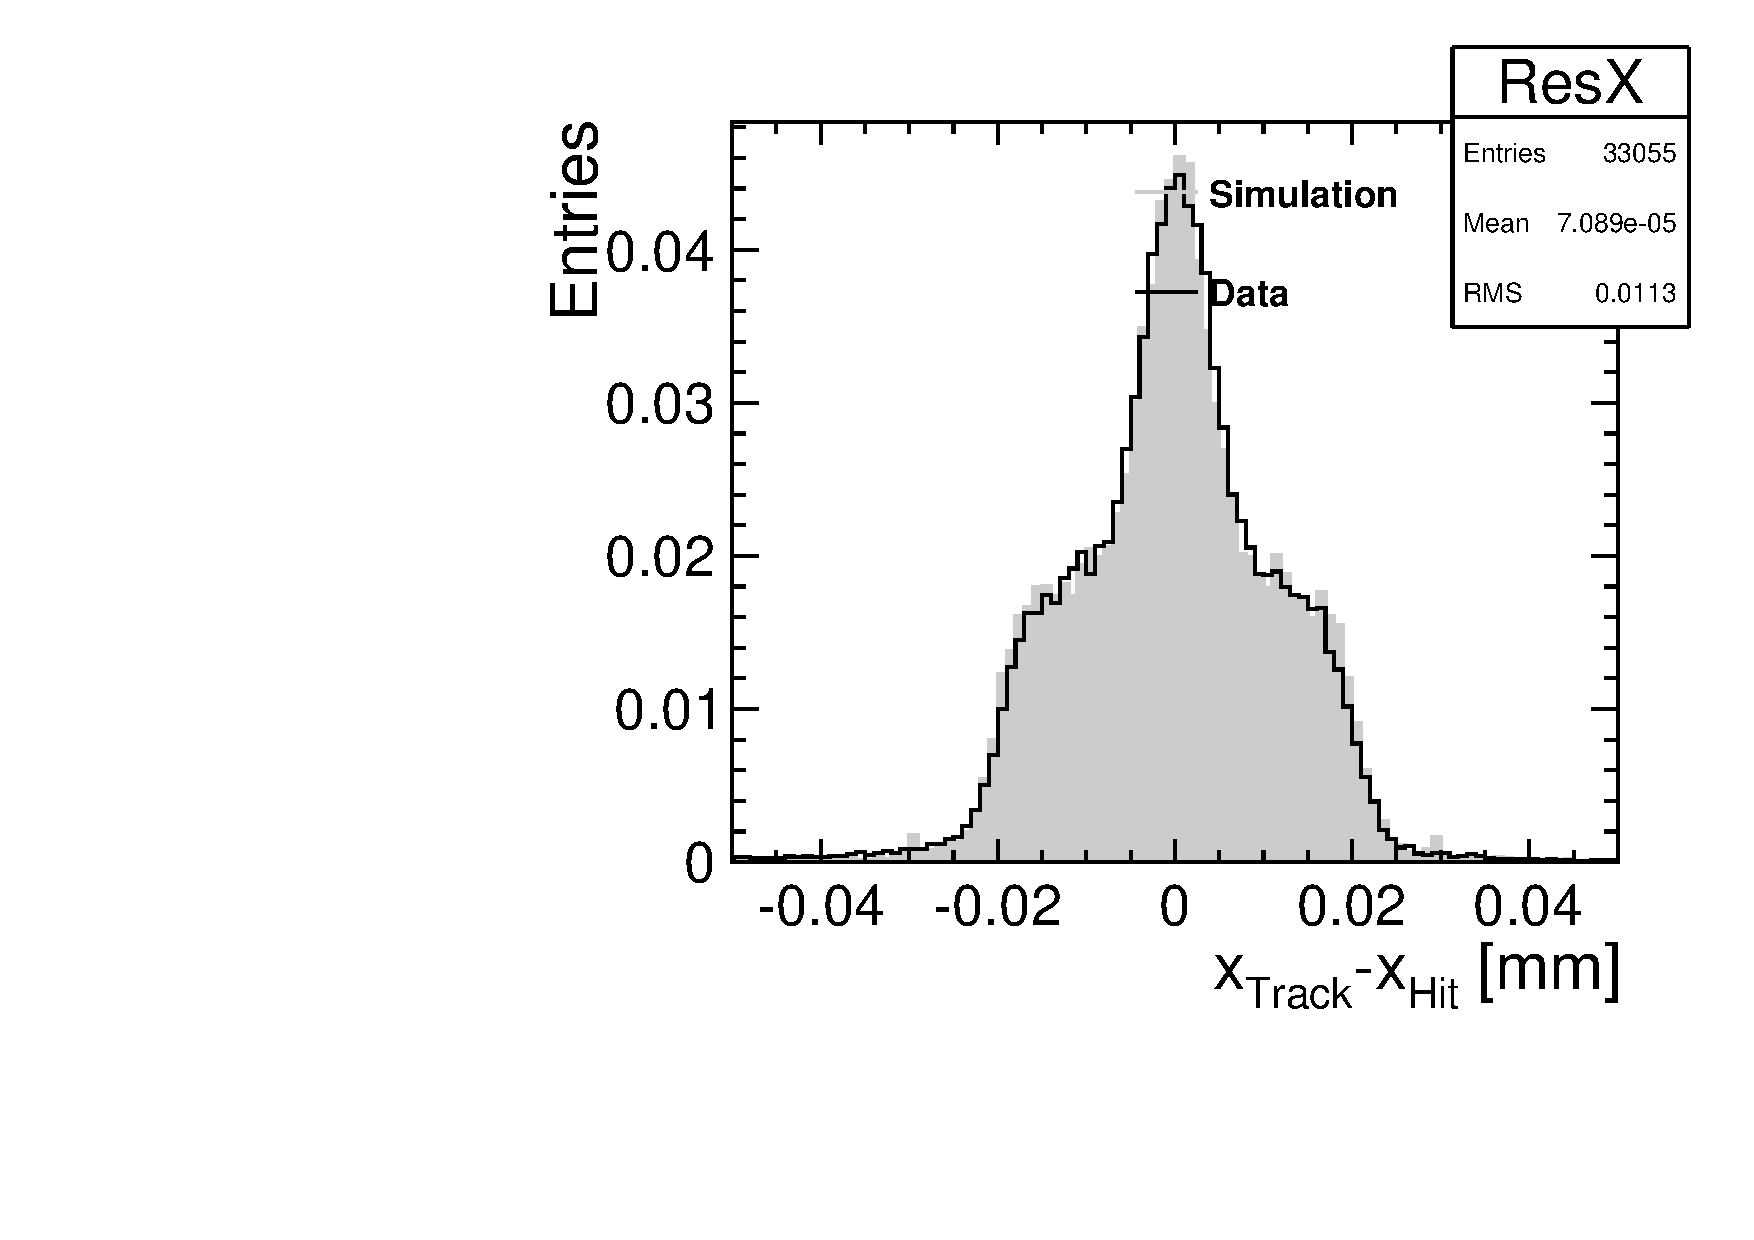
\includegraphics[width=0.8\textwidth]{../figures/TestBeam/150micron_resX.pdf}};
      \begin{scope}[x={(image.south east)},y={(image.north west)}]

        \node[below, color=black] at (0.55, 0.3) {Single-pixel};
        \node[below, color=black] at (0.35, 0.7) {Multi-pixel};
      \end{scope}
    \end{tikzpicture}
  \end{columns}

  \vspace{-1.3cm}

  \begin{columns}
    \column{0.5\textwidth}
    \begin{itemize}
    \item Good agreement between data and simulation
    \end{itemize}

    \column{0.5\textwidth}
    \centering
    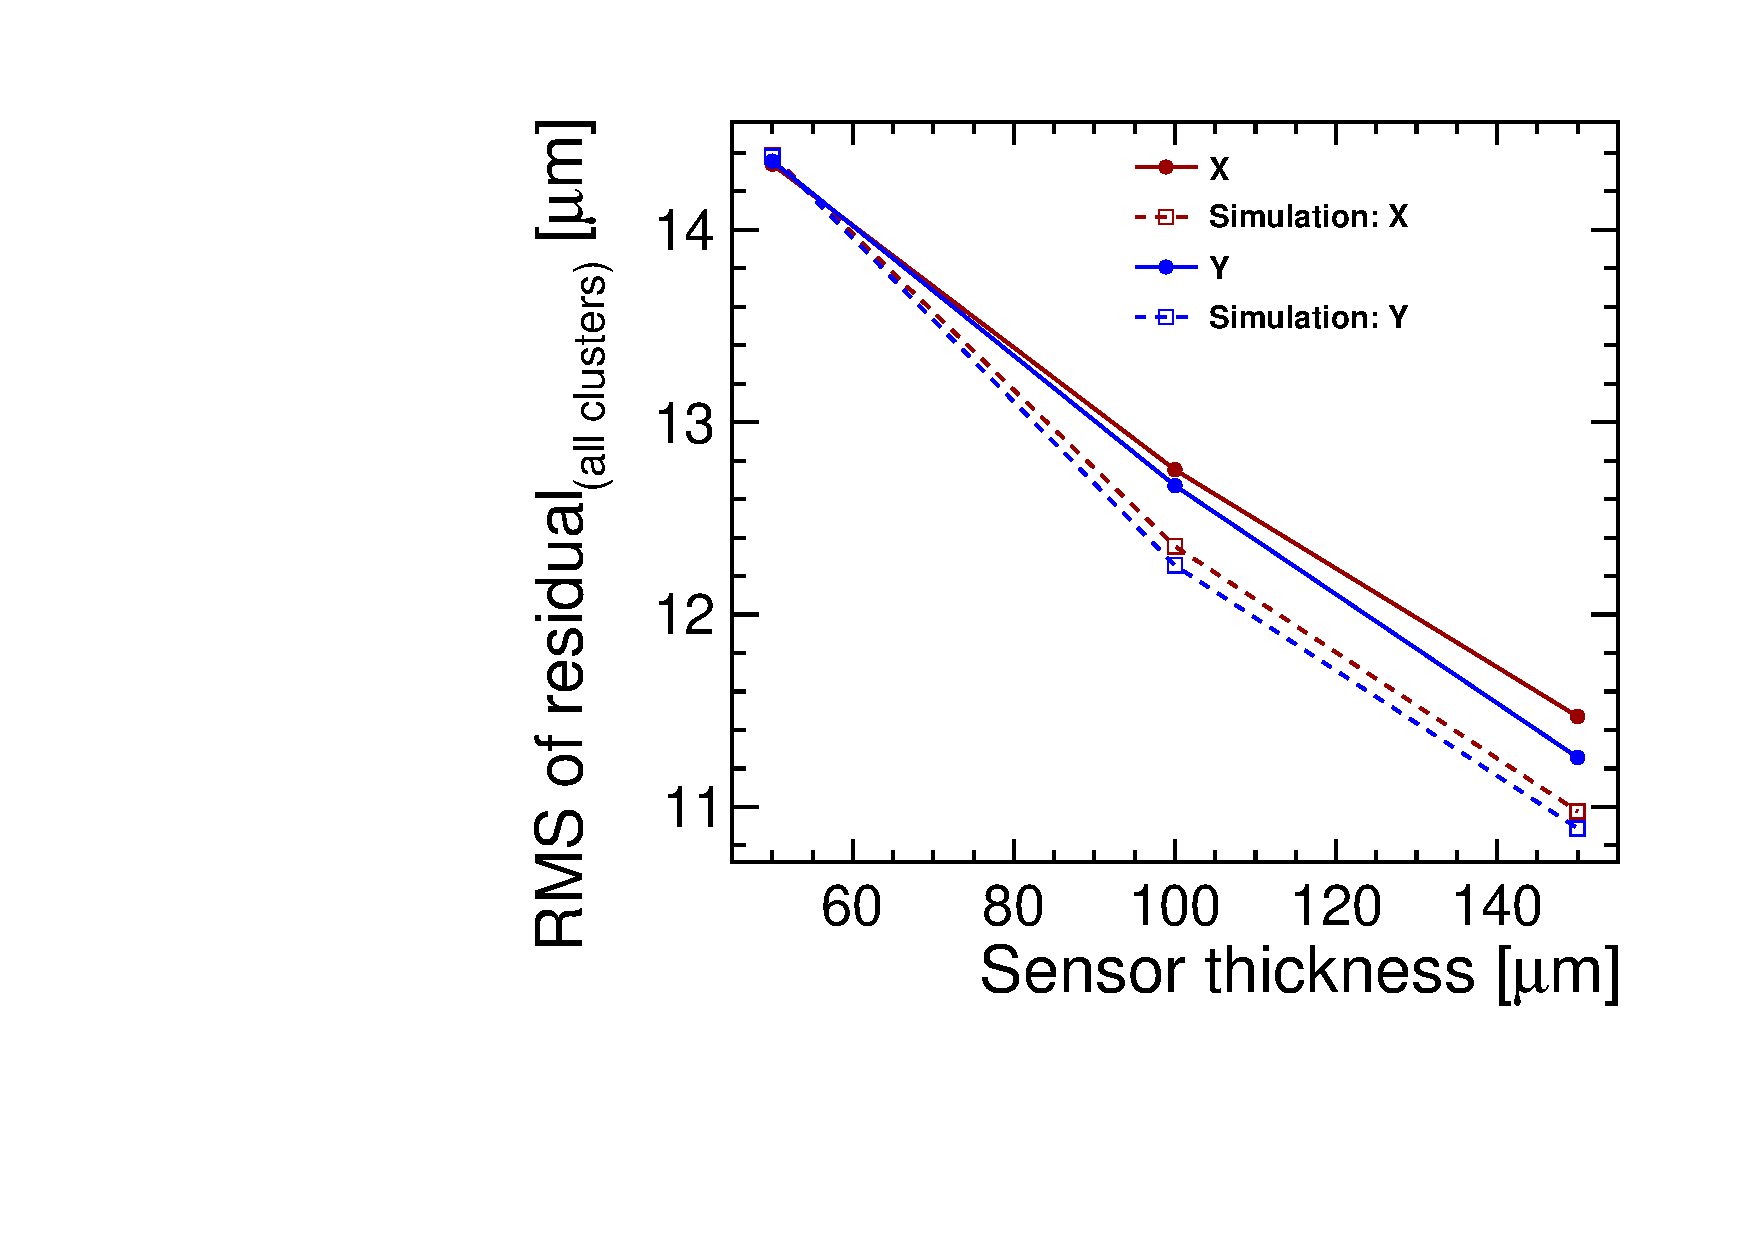
\includegraphics[width=0.8\textwidth]{../figures/TestBeam/residuals_vs_thickness.pdf}
  \end{columns}
  % \begin{columns}
  %   \column{0.5\textwidth}
  %   \begin{itemize}
  %   \item Detection efficiency as a function of the threshold
  %     of the readout ASIC.
  %   \end{itemize}

  %   \column{0.5\textwidth}
  %   \centering
  %   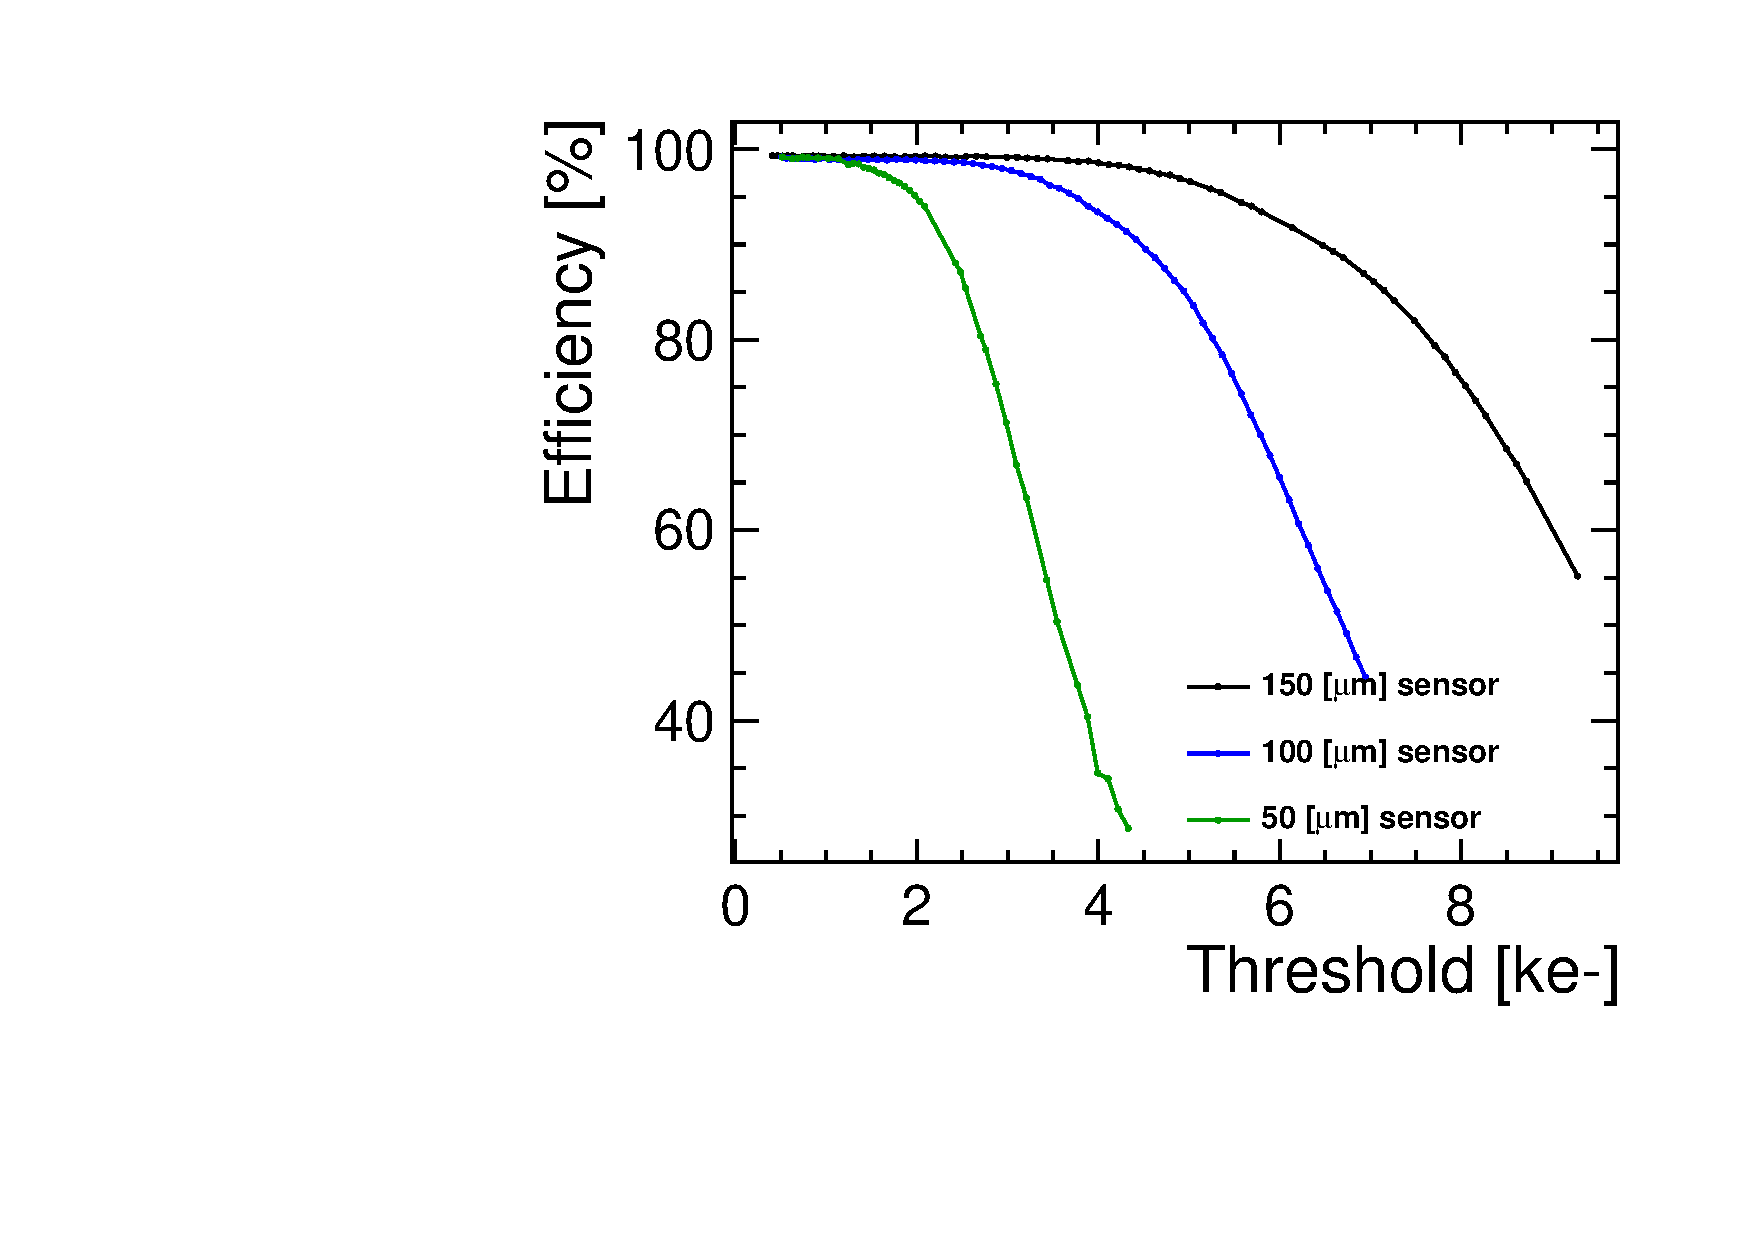
\includegraphics[width=0.8\textwidth]{../figures/TestBeam/Efficiency_vs_THL.pdf}
  % \end{columns}
  
\end{frame}


%%%%%%%%%%%%%%%%%%%%%%%%%%%%%
%         SLIDE             %
%%%%%%%%%%%%%%%%%%%%%%%%%%%%%
\begin{frame}
  \frametitle{Extrapolation of the simulation to smaller pixels}


  % \begin{itemize}
  % \item Small-pitch ASIC R\&D:
  %   \begin{itemize}
  %   \item CLICpix readout ASIC demonstrator
  %   \item Matrix of $64\times64$ pixels, $25\,\micron$ pixel pitch.
  %   \item 65~nm CMOS technology
  %   \item Simultaneous measurement of time (TOA) and energy (TOT) per
  %     pixel.
  %   \item Compatible with power pulsing scheme.
  %   \end{itemize}
  % \end{itemize}

  \begin{itemize}
  \item CLICpix readout ASIC demonstrator with $25\,\micron$ pitch
    under investigation
    % \begin{itemize}
    % \item Still, no data with $50\,\micron$ thick sensor is available
    % \end{itemize}
  \item Extrapolation of the simulation to smaller pixels:
    $10\,\micron$-$55\,\micron$ pitch
    \begin{itemize}
    \item For a $50\,\micron$ thick sensor and a Timepix3-like readout
      chip:
    \end{itemize}
  \end{itemize}
    
  \begin{columns}
    \column{0.5\textwidth}
    \centering
    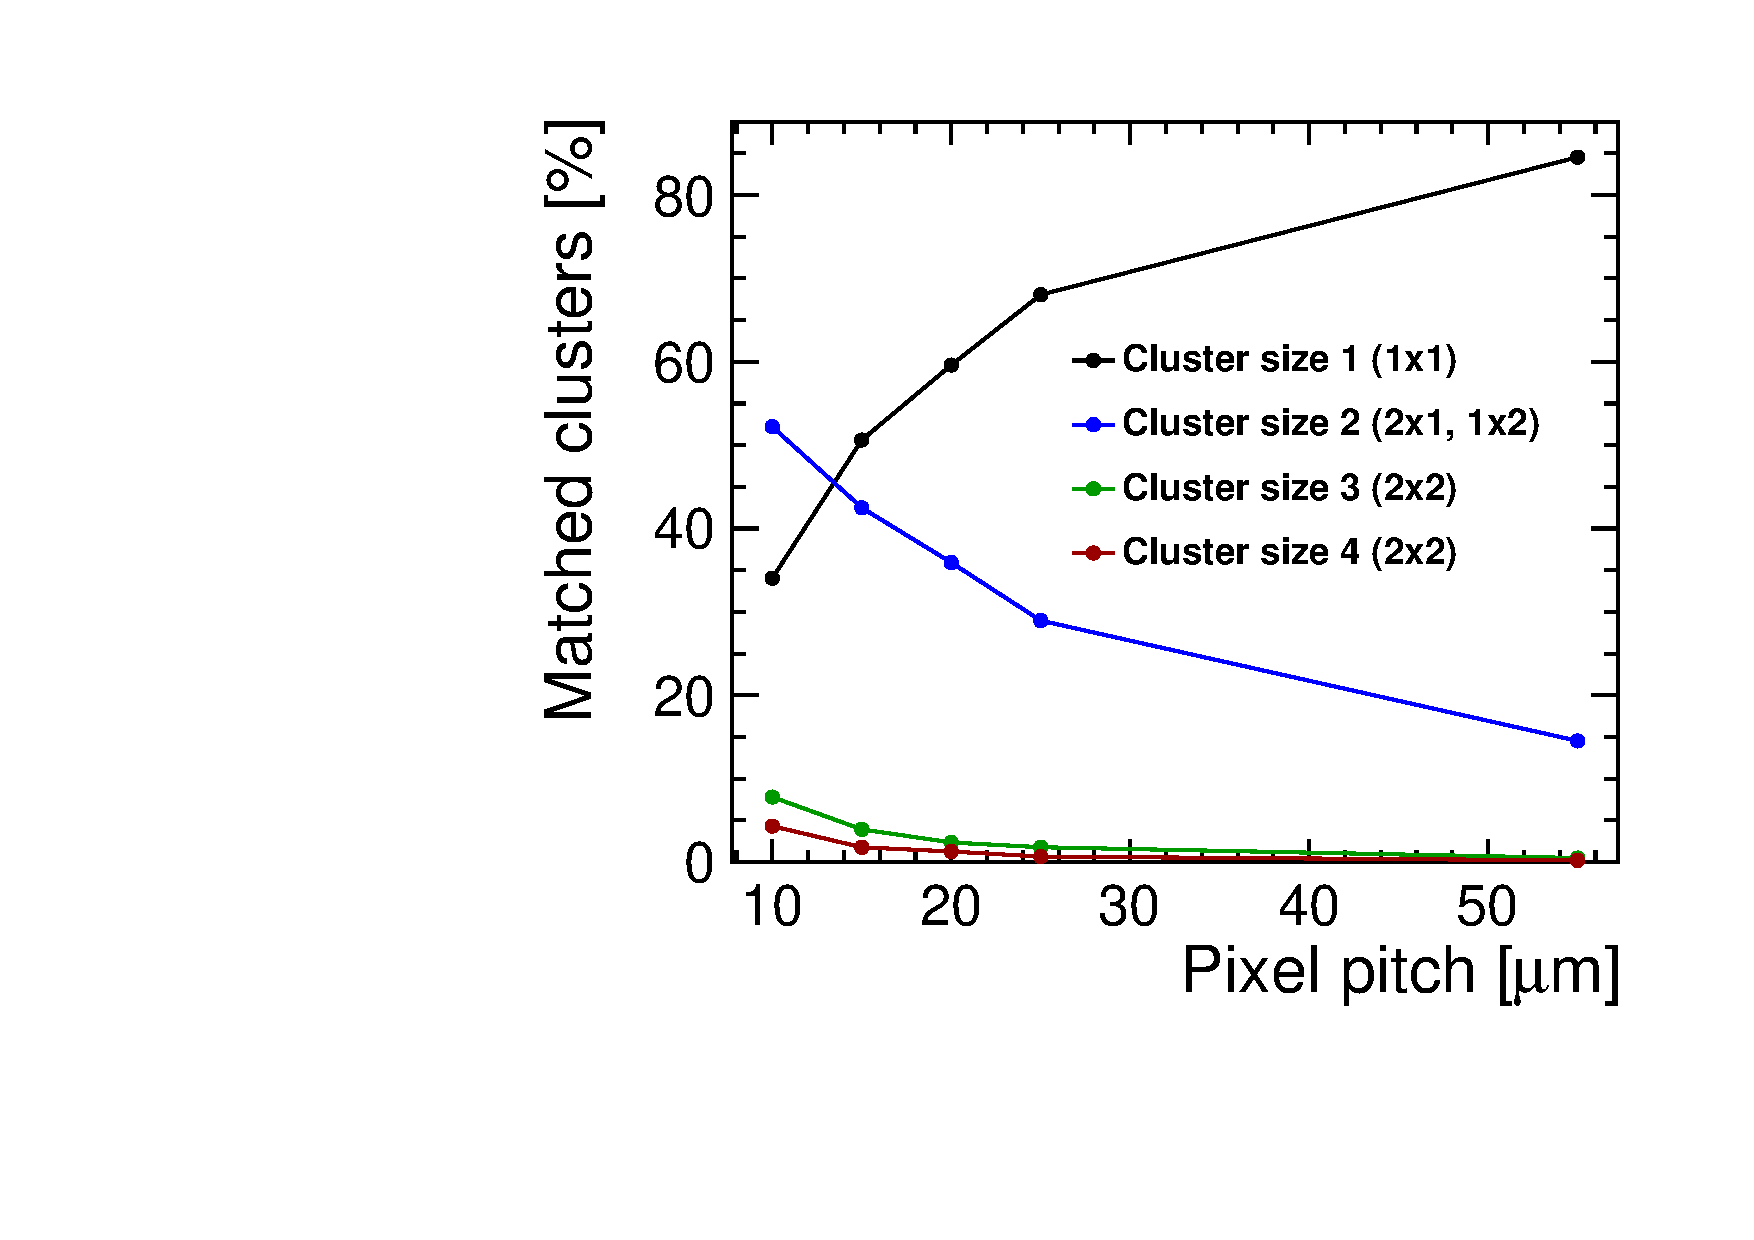
\includegraphics[width=\textwidth]{../figures/TestBeam/ClusterSize_extrapolationSmallerPixels.pdf}

    \column{0.5\textwidth}
    \centering
    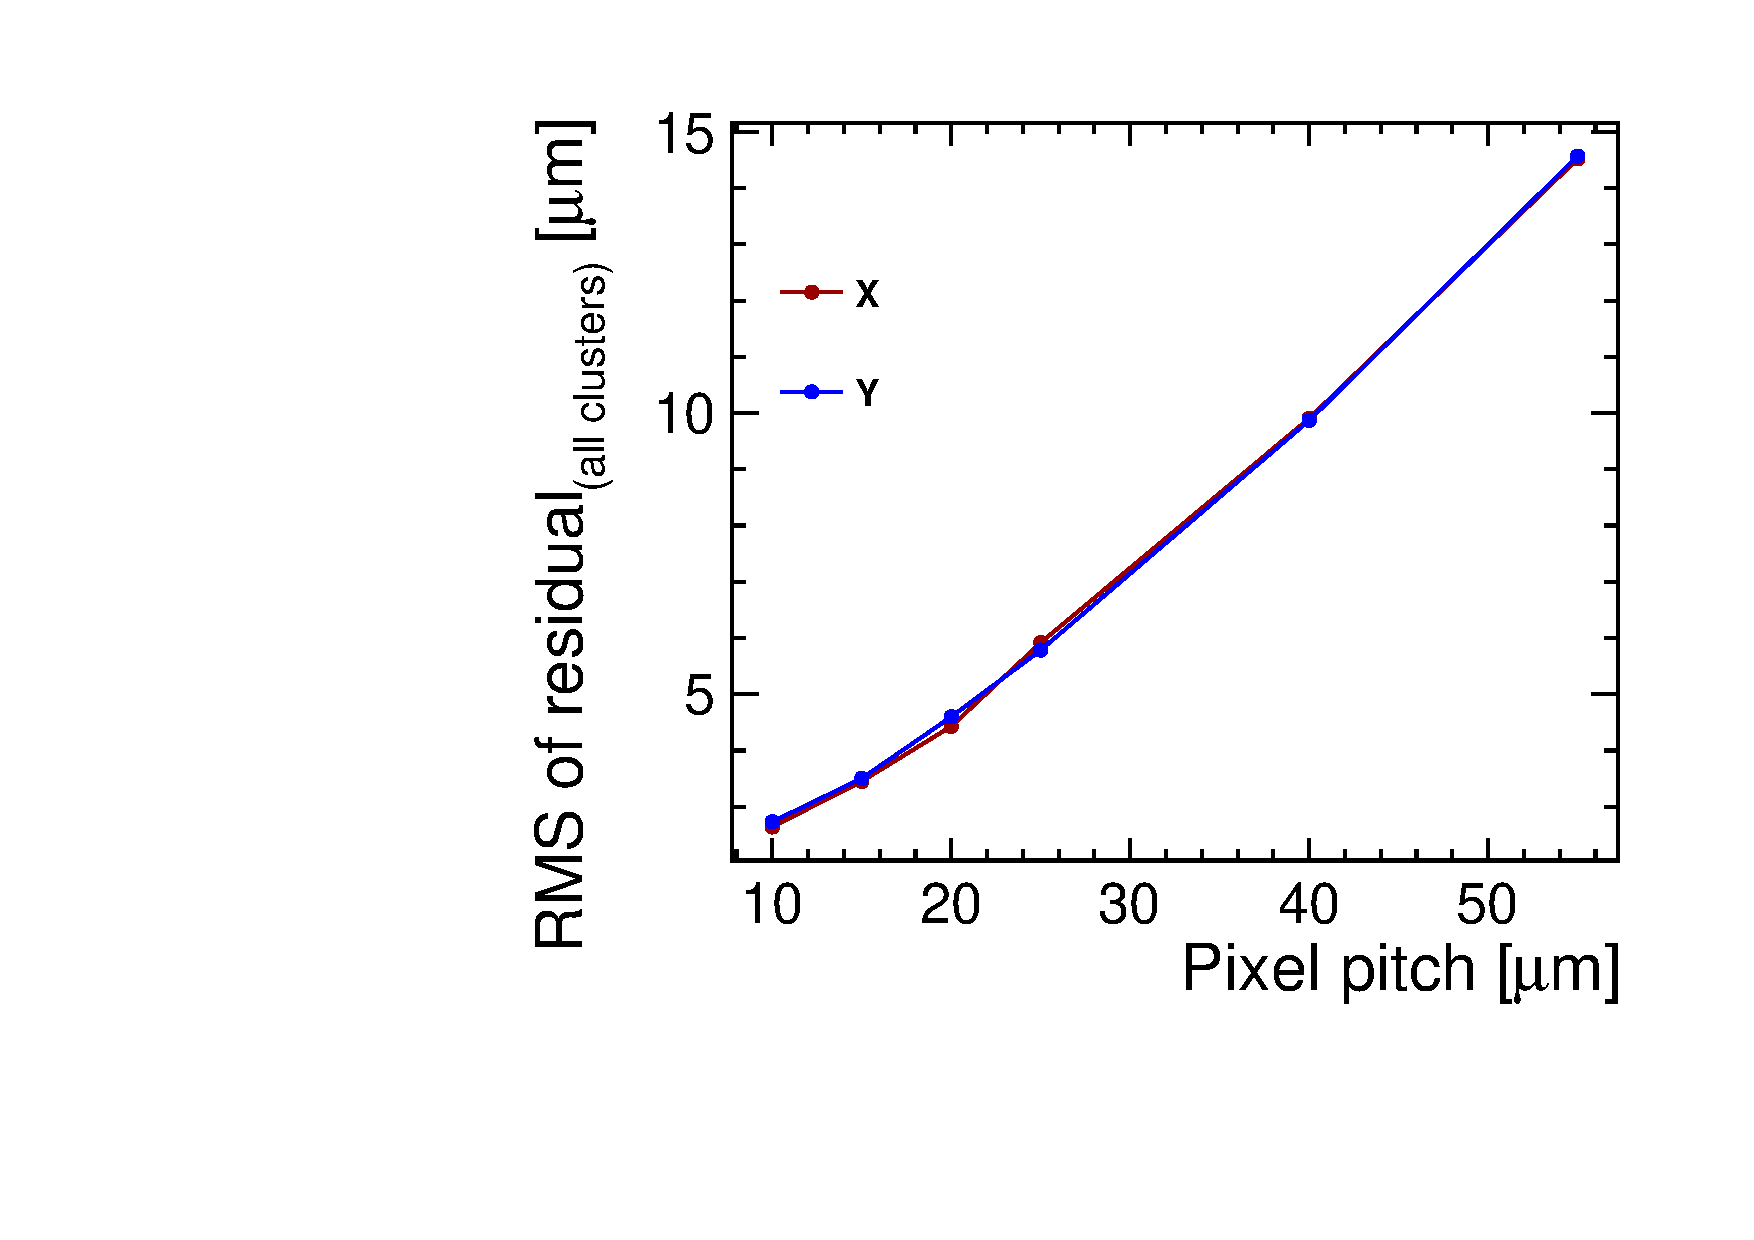
\includegraphics[width=\textwidth]{figures/extrapolation_resolution.pdf}
  \end{columns}

  \begin{itemize}
  \item For $25\,\micron$ pitch $\Rightarrow$ $\sim70\%$ single-pixel
    clusters, $\sigma\sim6\,\micron$
  \item $\sigma\sim3\,\micron$ can be achieved with:
    \begin{itemize} 
    \item Smaller pixels
      ($<15\,\micron$ pitch)
    \item New charge sharing solutions
    \end{itemize}
  \end{itemize}

\end{frame}

\section{Active-edge sensors}
\begin{frame}
  \frametitle{}
  \tableofcontents[currentsection]
\end{frame}
%%%%%%%%%%%%%%%%%%%%%%%%%%%%%
%         SLIDE             %
%%%%%%%%%%%%%%%%%%%%%%%%%%%%%
\begin{frame}
  \frametitle{Active-edge sensors}

  \begin{columns}
    \column{0.5\textwidth}

    \begin{itemize}
    \item Sawing sensors edges:
      \begin{itemize}
      \item Undefined edge
      \item Dangling bonds
      \item Short between surfaces 
      \end{itemize}

%      \centering
      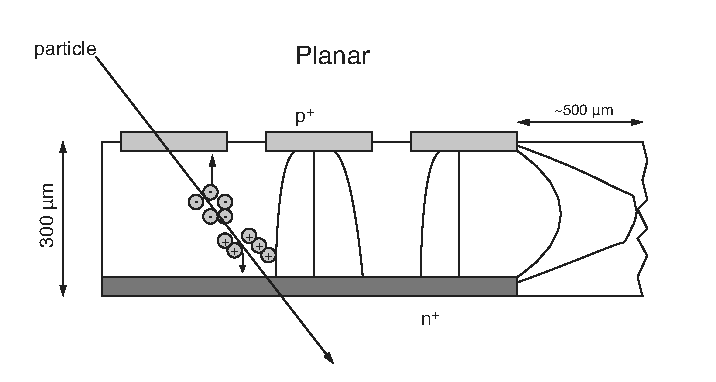
\includegraphics[width=\textwidth]{figures/sawing_planarSensor.pdf}

    \item Maximise the sensitive region of detectors with active-edge
      sensors
    \item Seamless tiling of pixel sensors:
      \begin{itemize}
      \item Avoid overlaps between the pixel sensors
      \item Reduce the material content in the detector
      \item High coverage
      \end{itemize}
    \end{itemize}

    \column{0.5\textwidth}
    \vspace{-0.8cm}
    \begin{tikzpicture}
      \node[anchor=south west,inner sep=0] (image) at (0,
      0){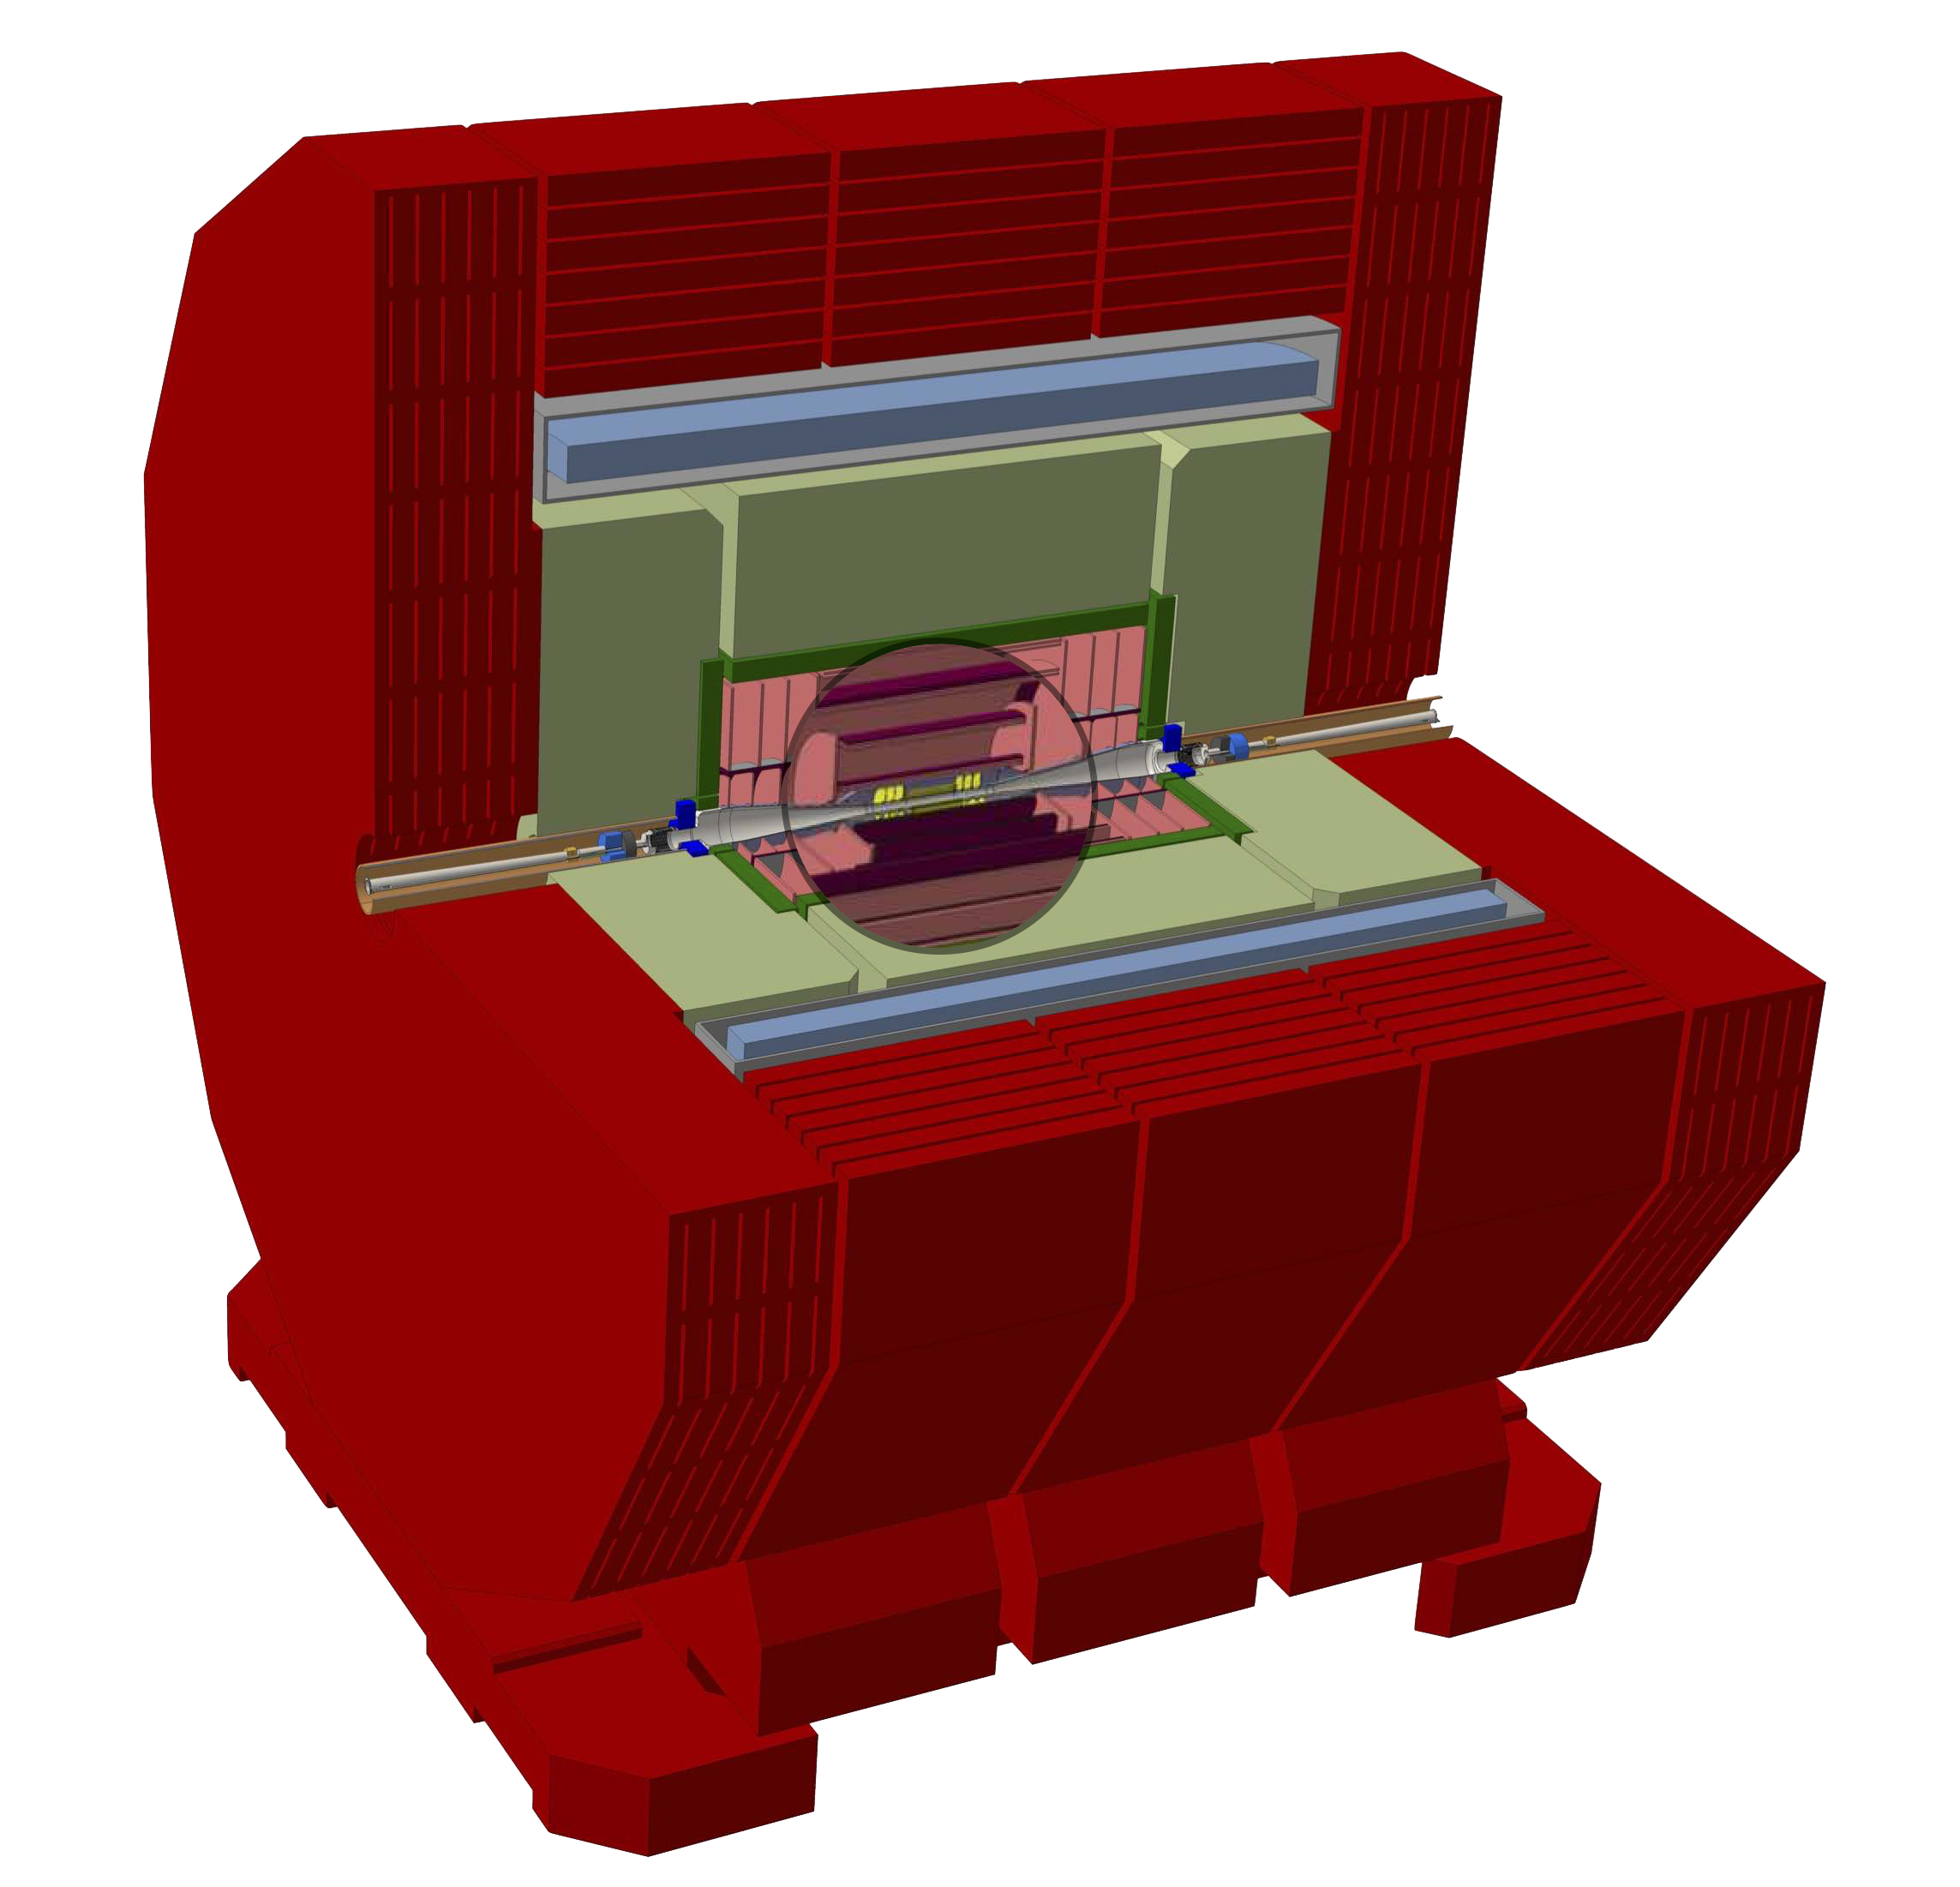
\includegraphics[width=\textwidth]{figures/CLIC_detector_2016_2.png}};
      \begin{scope}[x={(image.south east)},y={(image.north west)}]
        
        % \draw[help lines,xstep=.1,ystep=.1] (0, 0) grid (1,1);
        % \foreach \x in {0,1,...,9} { \node [anchor=north] at (\x/10,0) {0.\x}; }
        % \foreach \y in {0,1,...,9} { \node [anchor=east] at (0,\y/10)
        % {0.\y}; }

        \draw[<->,line width=0.5pt] (0.15, 0.95) -- (0.7, 0.99);
        \node[color=black] at (0.45, 1) {11.4~m};
        
        % \draw[<->,line width=0.5pt] (0.04, 0.17) -- (0.04, 0.9);
        % \node[color=black, rotate=90] at (0.01, 0.5) {12.9~m};
        
        \node[color=white] at (0.45, 0.9) {\textbf{CLIC detector}};
        \draw[->,line width=1.7pt] (0.5, 0.5) -- (0.5, 0.33);
        %\node[color=black] at (0.58, 0.43) {\textbf{VXD}};

      \end{scope}
    \end{tikzpicture}

    \vspace{-1.5cm}
    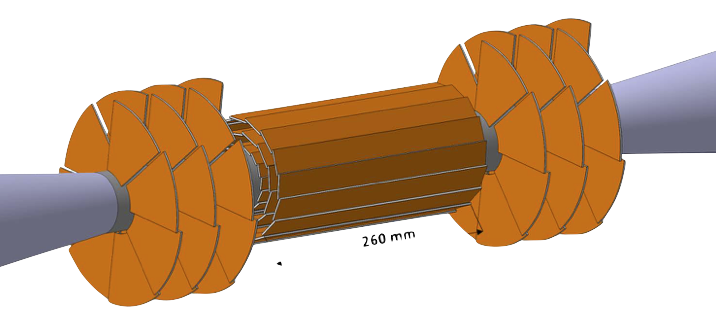
\includegraphics[width=\textwidth]{figures/spiralVXD_2.png}\\

    \vspace{-0.8cm}
    \begin{adjustbox}{max totalsize={.9\textwidth}{.4\textheight},center}
      \begin{tikzpicture}[node distance = 2.5cm, auto]
        \begin{scope}[x={(image.south east)},y={(image.north west)}]
          
          % \draw[help lines,xstep=.1,ystep=.1] (0, 0) grid (1,1);
          % \foreach \x in {0,1,...,9} { \node [anchor=north] at (\x/10,0) {0.\x}; }
          % \foreach \y in {0,1,...,9} { \node [anchor=east] at (0,\y/10)
          %   {0.\y}; }
          
          \draw[->,line width=1.7pt] (0.5, 1.15) -- (0.5, 1);
          \node[color=black] at (0.65, 1.1) {\textbf{Ladders}};

          \draw[thick, fill=Orange] (0.05, 0.45) rectangle (0.95, 0.95);

          \draw[very thick, fill=gray] (0.1, 0.7) rectangle (0.3, 0.9);

          % \draw[-,line width=0.1pt] (0.15, 0.7) -- (0.15, 0.9);
          % \draw[-,line width=0.1pt] (0.2, 0.7) -- (0.2, 0.9);
          % \draw[-,line width=0.1pt] (0.25, 0.7) -- (0.25, 0.9);
          % \draw[-,line width=0.1pt] (0.1, 0.8) -- (0.3, 0.8);
          % \draw[-,line width=0.1pt] (0.1, 0.85) -- (0.3, 0.85);
          % \draw[-,line width=0.1pt] (0.1, 0.75) -- (0.3, 0.75);

          \draw[very thick, fill=gray] (0.1, 0.5) rectangle (0.3,
          0.7);


          % \draw[-,line width=0.1pt] (0.15, 0.5) -- (0.15, 0.7);
          % \draw[-,line width=0.1pt] (0.2, 0.5) -- (0.2, 0.7);
          % \draw[-,line width=0.1pt] (0.25, 0.5) -- (0.25, 0.7);
          % \draw[-,line width=0.1pt] (0.1, 0.65) -- (0.3, 0.65);
          % \draw[-,line width=0.1pt] (0.1, 0.6) -- (0.3, 0.6);
          % \draw[-,line width=0.1pt] (0.1, 0.55) -- (0.3, 0.55);


          \draw[very thick, fill=gray] (0.3, 0.7) rectangle (0.5, 0.9);
          \draw[very thick, fill=gray] (0.3, 0.5) rectangle (0.5, 0.7);
          \draw[very thick, fill=gray] (0.5, 0.7) rectangle (0.7, 0.9);
          \draw[very thick, fill=gray] (0.5, 0.5) rectangle (0.7, 0.7);
          \draw[very thick, fill=gray] (0.7, 0.7) rectangle (0.9, 0.9);
          \draw[very thick, fill=gray] (0.7, 0.5) rectangle (0.9, 0.7);

        \end{scope}
      \end{tikzpicture}
    \end{adjustbox}
    
  \end{columns}
\end{frame}

\subsection{Fabrication process}
\begin{frame}
  \frametitle{}
  \tableofcontents[currentsubsection]
\end{frame}
%%%%%%%%%%%%%%%%%%%%%%%%%%%%%
%         SLIDE             %
%%%%%%%%%%%%%%%%%%%%%%%%%%%%%
\begin{frame}
  \frametitle{Fabrication process}

  \begin{itemize}
  \item The \textcolor{Blue}{DRIE} (Deep Reactive-Ion Etching) process
    is used to cut an active-edge silicon sensor.
  \item Implantation on the sidewall of the sensor $\Rightarrow$
    control the potential at the edge by creating an extension of the
    backside electrode on the edge.
  \item Guard rings (GR): metal and n-implants to establish a smooth
    voltage drop between the edge and the last pixel.
  \end{itemize}

  \begin{columns}
    \column{0.5\textwidth}

    \begin{tikzpicture}
      \node[anchor=south west,inner sep=0] (image) at
      (0,0){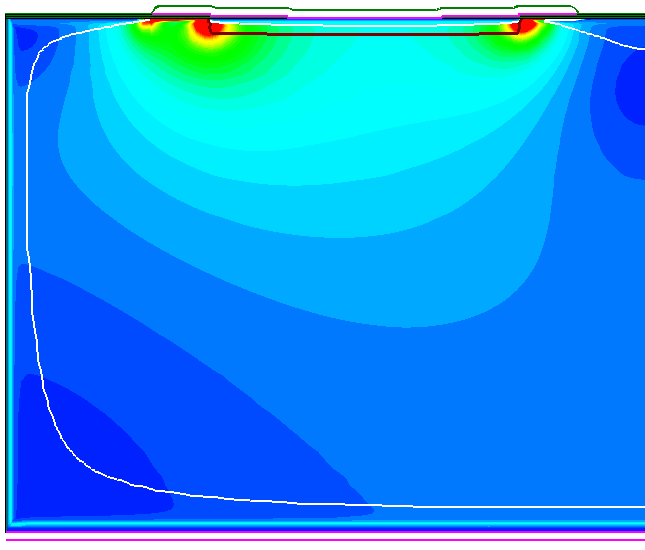
\includegraphics[width=0.78\textwidth]{figures/Efield_20_NGR.png}};
      \begin{scope}[x={(image.south east)},y={(image.north west)}]
        \draw[-, dashed, line width=.7pt, color=white](0.1, 0.05) -- (0.1, 0.92);
        % \draw[-, dashed, line width=.7pt, color=white](0.54, 0.05) -- (0.54, 0.92);
        
        \draw[<->, line width=.7pt, color=black](0.01, 1) -- (0.32, 1); % edge width
        \node[above, color=black] at (0.1, 1) {edge};
        
        \draw[<->, thick, color=black](0.33, 1) -- (0.8, 1); % n-implant
        \node[above, color=black] at (0.6, 1) {n-implant};

        \node[above, color=white] at (0.5, 0.5) {\textbf{p-substrate}};
        
        \draw[-, line width=3pt, color=violet](0.0, 0.05) -- (0.98, 0.05); % p+ backside contact
        \node[below, color=violet] at (0.5, 0.0) {p+ backside contact};
        \draw[-, line width=3pt, color=violet](0.0, 0.045) -- (0.0, 0.93); % p+ active-edge contact
        \node[left, color=violet, rotate=90] at (-0.05, 0.7) {p+ active edge};
        % \node[left, color=white, rotate=90] at (0.08, 0.9) {\textbf{final pixel edge}};

        % \draw[help lines,xstep=.1,ystep=.1] (0, 0) grid (1,1);
        % \foreach \x in {0,1,...,9} { \node [anchor=north] at (\x/10,0) {0.\x}; }
        % \foreach \y in {0,1,...,9} { \node [anchor=east] at (0,\y/10) {0.\y}; }
      \end{scope}
    \end{tikzpicture}

    \column{0.5\textwidth}
    \begin{tikzpicture}
      \node[anchor=south west,inner sep=0] (image) at
      (0,0){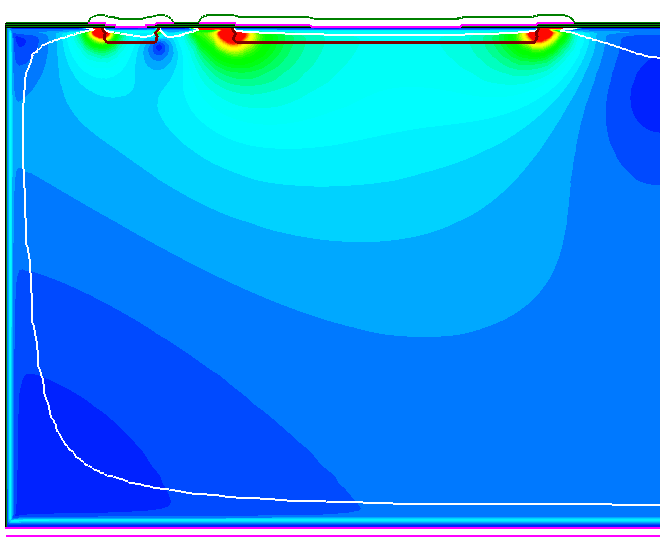
\includegraphics[width=0.8\textwidth]{figures/Efield_23_FGR.png}};
      \begin{scope}[x={(image.south east)},y={(image.north west)}]
        \draw[-, dashed, line width=.7pt, color=white](0.14, 0.05) -- (0.14, 0.92);
        % \draw[-, dashed, line width=.7pt, color=white](0.54, 0.05) -- (0.54, 0.92);
        \draw[<->, line width=.7pt, color=black](0.01, 1) -- (0.35, 1); % edge width
        
        \node[above, color=black] at (0.2, 1) {edge};
        \node[above, color=white] at (0.2, 0.75) {\textbf{GR}};
        \node[above, color=white] at (0.55, 0.5) {\textbf{p-substrate}};
        \draw[<->, line width=.4pt, color=black](0.13, 0.0) -- (0.98, 0.0); % pixel width
        \node[below, color=black] at (0.5, 0.0) {\small{pixel (55
            \micron)}};

        \draw[<->, thick, color=black](0.36, 1) -- (0.81, 1); % n-implant
        \node[above, color=black] at (0.6, 1) {n-implant};
        
        \draw[-, line width=3pt, color=violet](0.01, 0.05) -- (0.99, 0.05); % p+ backside contact
        \draw[-, line width=3pt, color=violet](0.01, 0.045) -- (0.01,
        0.95); % p+ active-edge contact

        % \draw[help lines,xstep=.1,ystep=.1] (0, 0) grid (1,1);
        % \foreach \x in {0,1,...,9} { \node [anchor=north] at (\x/10,0) {0.\x}; }
        % \foreach \y in {0,1,...,9} { \node [anchor=east] at (0,\y/10) {0.\y}; }
      \end{scope}
    \end{tikzpicture}
  \end{columns}

\end{frame}

%%%%%%%%%%%%%%%%%%%%%%%%%%%%%
%         SLIDE             %
%%%%%%%%%%%%%%%%%%%%%%%%%%%%%
\begin{frame}
  \frametitle{Guard-ring designs and TCAD simulations}

  \begin{itemize}
  \item 4 assemblies with $50\,\micron$-thick sensors: No GR, floating
    and grounded potentials GR.
  \end{itemize}

  \vspace{-0.3cm}
  \begin{columns}[t]
    \column{0.23\textwidth}
    \begin{itemize}
    %\item 20-NGR-50
    \item No GR \\
      $\Rightarrow$ $20\,\micron$ edge
    \end{itemize}
    \centering
    \begin{tikzpicture}
      \node[anchor=south west,inner sep=0] (image) at
      (0,0){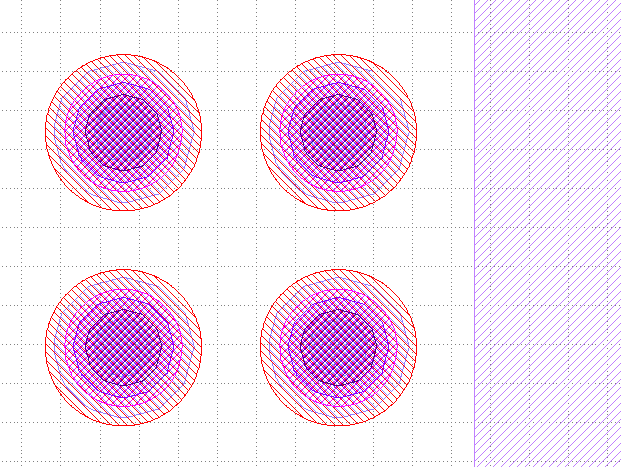
\includegraphics[width=0.8\textwidth]{figures/Layout2Pixels2.png}};
      \begin{scope}[x={(image.south east)},y={(image.north west)}]
        % \node[above] at (0.8, 0.7) {\small{\SI{15}{\micro\meter}}};
        \draw[Blue, thick](0.765, 0.05)--(0.765, 0.95);
        \draw[Blue, thick, dashed](0.7, 0.05)--(0.7, 0.95);
        \draw[Blue, thick](0.38, 0.05)--(0.38, 0.95);
        \draw[Blue, thick](0.98, 0.05)--(0.98, 0.95);
        \draw[Blue, thick](0.38, 0.05)--(0.98, 0.05);
        \draw[Blue, thick](0.38, 0.95)--(0.98, 0.95);
        \node[below, color=Blue] at (0.38, 0.055) {-0.055};
        \node[below, color=Blue] at (0.7, 0.055) {0};
        \node[below, color=Blue] at (0.98, 0.055) {0.055};
      \end{scope}
    \end{tikzpicture}


    \column{0.27\textwidth}
    \begin{itemize}
%    \item 28-GNDGR-50
    \item Grounded GR \\
      $\Rightarrow$ $28\,\micron$ edge  
  \end{itemize}
    \centering
    \begin{tikzpicture}
      \node[anchor=south west,inner sep=0] (image) at
      (0,0){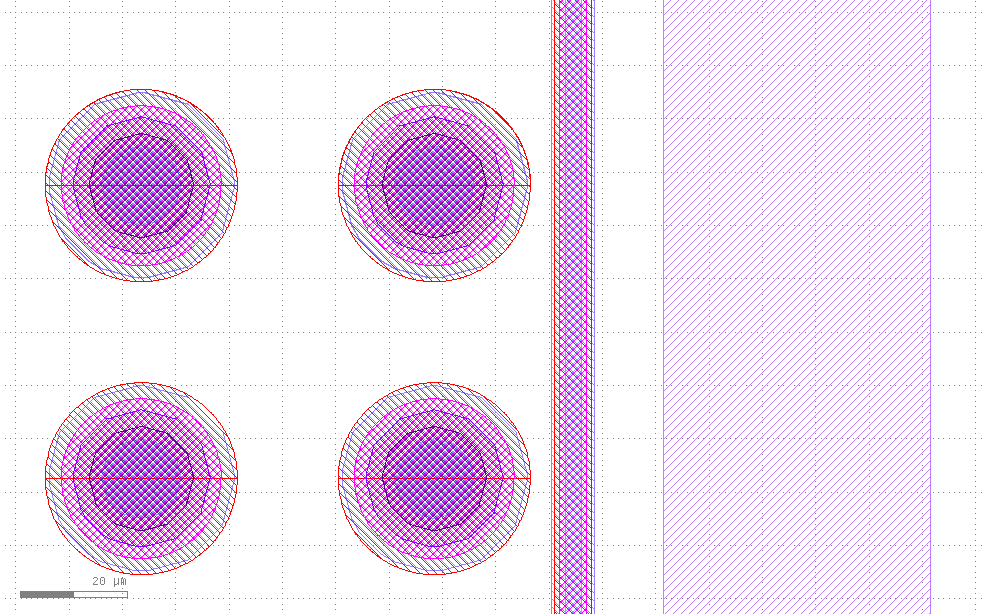
\includegraphics[width=0.8\textwidth]{figures/20_edge_GRND_GR_2.png}};
      \begin{scope}[x={(image.south east)},y={(image.north west)}]
        \draw[Blue, thick](0.68, 0.05)--(0.68, 0.95);
        \draw[Blue, thick, dashed](0.55, 0.05)--(0.55, 0.95);
        \draw[Blue, thick](0.3, 0.05)--(0.3, 0.95);
        \draw[Blue, thick](0.9, 0.05)--(0.9, 0.95);
        \draw[Blue, thick](0.3, 0.05)--(0.9, 0.05);
        \draw[Blue, thick](0.3, 0.95)--(0.9, 0.95);
        \node[below, color=Blue] at (0.3, 0.055) {-0.055};
        \node[below, color=Blue] at (0.55, 0.055) {0};
        \node[below, color=Blue] at (0.9, 0.055) {0.055};
      \end{scope}
    \end{tikzpicture}

    \column{0.27\textwidth}
    \begin{itemize}
    %\item 55-GNDGR-50
    \item Grounded GR \\
      $\Rightarrow$ $55\,\micron$ edge
    \end{itemize}
    \centering
    \begin{tikzpicture}
      \node[anchor=south west,inner sep=0] (image) at
      (0,0){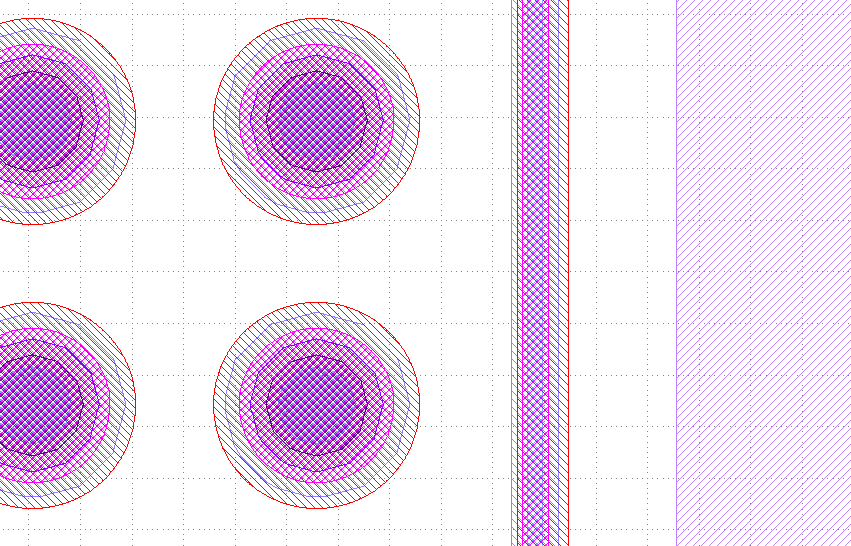
\includegraphics[width=0.8\textwidth]{{figures/50_edge_GRND_GR_2.png}}};
      \begin{scope}[x={(image.south east)},y={(image.north west)}]
        \draw[Blue, thick](0.8, 0.05)--(0.8, 0.95);
        \draw[Blue, thick, dashed](0.55, 0.05)--(0.55, 0.95);
        \draw[Blue, thick](0.25, 0.05)--(0.25, 0.95);
        \draw[Blue, thick](0.9, 0.05)--(0.9, 0.95);
        \draw[Blue, thick](0.25, 0.05)--(0.9, 0.05);
        \draw[Blue, thick](0.25, 0.95)--(0.9, 0.95);
        \node[below, color=Blue] at (0.25, 0.055) {-0.055};
        \node[below, color=Blue] at (0.55, 0.055) {0};
        \node[below, color=Blue] at (0.9, 0.055) {0.055};
      \end{scope}
    \end{tikzpicture}


    \column{0.23\textwidth}
    \begin{itemize}
    % \item 23-FGR-50
    \item Floating GR \\
      $\Rightarrow$ $23\,\micron$ edge
    \end{itemize}
    \centering
    \begin{tikzpicture}
      \node[anchor=south west,inner sep=0] (image) at
      (0,0){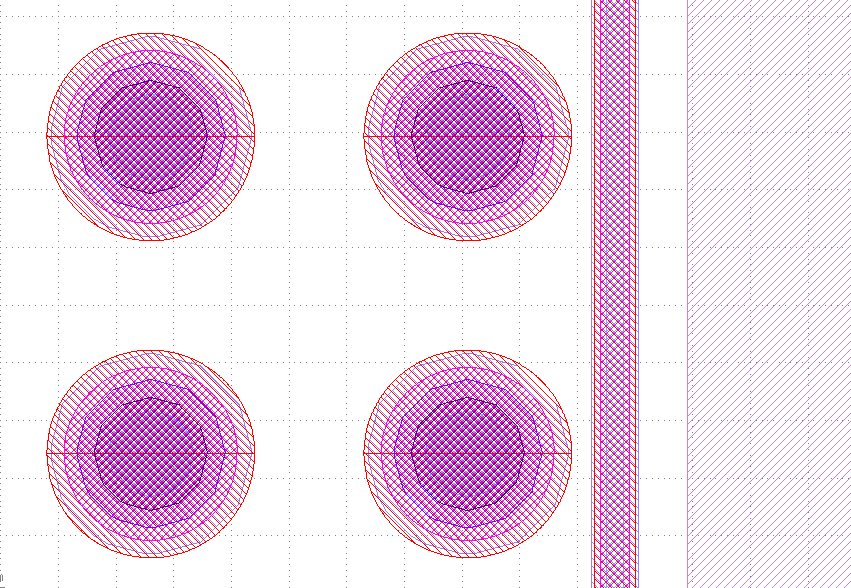
\includegraphics[width=0.8\textwidth]{figures/20_edge_float_GR_3.png}};
      \begin{scope}[x={(image.south east)},y={(image.north west)}]
        % \node[above] at (0.8, 0.7) {\small{\SI{20}{\micro\meter}}};
        \draw[Blue, thick](0.8, 0.05)--(0.8, 0.95);
        \draw[Blue, thick, dashed](0.7, 0.05)--(0.7, 0.95);
        \draw[Blue, thick](0.4, 0.05)--(0.4, 0.95);
        \draw[Blue, thick](1, 0.05)--(1, 0.95);
        \draw[Blue, thick](0.4, 0.05)--(1, 0.05);
        \draw[Blue, thick](0.4, 0.95)--(1, 0.95);
        \node[below, color=Blue] at (0.4, 0.055) {-0.055};
        \node[below, color=Blue] at (0.7, 0.055) {0};
        \node[below, color=Blue] at (1, 0.055) {0.055};
      \end{scope}
    \end{tikzpicture}

  \end{columns}

  \begin{itemize}
  \item 2 assemblies with grounded GR: $100\,\micron$ and
    $150\,\micron$ thick sensors.
  \end{itemize}

  \begin{columns}[t]
    \column{0.5\textwidth}
    \begin{itemize}
    \item TCAD simulations:
      \begin{itemize}
      \item Finite element methods to numerically solve continuity and
        diffusion equations in semiconductors.
      \item Simulation of \textcolor{Green}{semiconductor processing}
        \& \textcolor{Green}{device operation}.
      \end{itemize}
    \end{itemize}

    \column{0.5\textwidth}
    \begin{itemize}
    \item Transient simulation of a particle track traversing the
      sensor
    \end{itemize}

    \centering
    \begin{tikzpicture}
      \node[anchor=south west,inner sep=0] (image) at
      (0,0){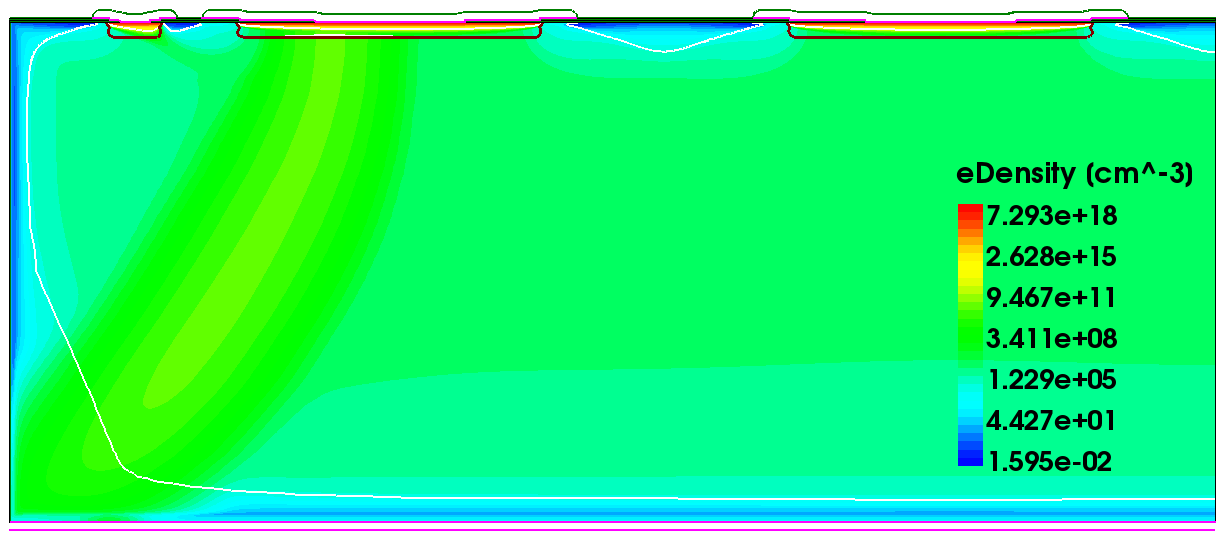
\includegraphics[width=\textwidth]{../figures/ActiveEdge/TCAD_transient_23FGR_hitpos_60.png}};
      \begin{scope}[x={(image.south east)},y={(image.north west)}]
        \draw[->, very thick] (0.093, 0.0) -- (0.093, 1.05);
      \end{scope}
    \end{tikzpicture}
  \end{columns}

\end{frame}

\subsection{Edge performance in data and simulations}
\begin{frame}
  \frametitle{}
  \tableofcontents[currentsubsection]
\end{frame}
%%%%%%%%%%%%%%%%%%%%%%%%%%%%%
%         SLIDE             %
%%%%%%%%%%%%%%%%%%%%%%%%%%%%%
\begin{frame}
  \frametitle{Active-edge sensor without GR (20-NGR-50)}

  \begin{columns}
    \column{0.5\textwidth}

    \begin{itemize}
    \item Efficient up to the physical edge.
    \item All the generated charge is collected by the pixel implant.
    \end{itemize}


    \column{0.5\textwidth}

    \begin{columns}
      \column{0.5\textwidth}
      \centering
      \begin{tikzpicture}
        \node[anchor=south west,inner sep=0] (image) at
        (0,0){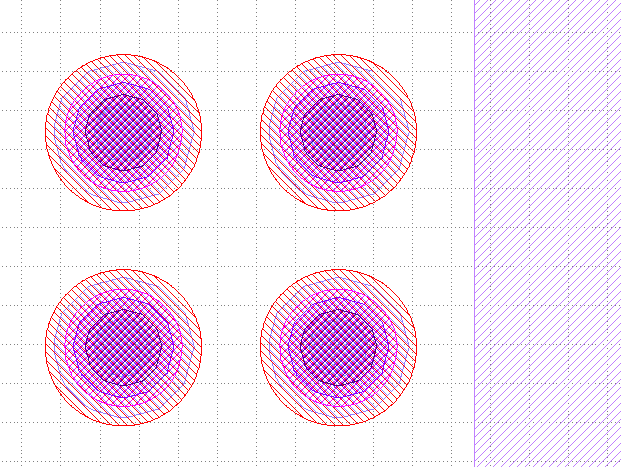
\includegraphics[width=\textwidth]{figures/Layout2Pixels2.png}};
        \begin{scope}[x={(image.south east)},y={(image.north west)}]
          % \node[above, color=Blue, rotate=90] at (0.1, 0.5)
          % {\small{\textbf{20-NGR}}};
          % \node[above, color=Blue, rotate=90] at (0.25, 0.5) {\small{(no GR)}};
          % \node[above] at (0.8, 0.7) {\small{\SI{15}{\micro\meter}}};
          \draw[Blue, thick](0.765, 0.05)--(0.765, 0.95);
          \draw[Blue, thick, dashed](0.7, 0.05)--(0.7, 0.95);
          \draw[Blue, thick](0.38, 0.05)--(0.38, 0.95);
          \draw[Blue, thick](0.98, 0.05)--(0.98, 0.95);
          \draw[Blue, thick](0.38, 0.05)--(0.98, 0.05);
          \draw[Blue, thick](0.38, 0.95)--(0.98, 0.95);
          \node[below, color=Blue] at (0.38, 0.055) {-0.055};
          \node[below, color=Blue] at (0.7, 0.055) {0};
          \node[below, color=Blue] at (0.98, 0.055) {0.055};
        \end{scope}
      \end{tikzpicture}
      \column{0.5\textwidth}
      \centering
      \reflectbox{\includegraphics[width=\textwidth]{../figures/ActiveEdge/streamlines_20-NGR-50.png}}
    \end{columns}

  \end{columns}

  \begin{columns}[t]
    \column{0.5\textwidth}
    
    \begin{itemize}
    \item Efficiency vs. track position
    \end{itemize}
    \centering
    \includegraphics[width=\textwidth, page=3]{../figures/TestBeam/edge_bcp.pdf}
    
    \column{0.5\textwidth}
    \begin{itemize}
    \item Energy deposition vs. track position
    \end{itemize}
    \centering
    \includegraphics[width=\textwidth]{../figures/ActiveEdge/20_NGR_Edep_TCAD_data.pdf}

  \end{columns}

\end{frame}




%%%%%%%%%%%%%%%%%%%%%%%%%%%%%
%         SLIDE             %
%%%%%%%%%%%%%%%%%%%%%%%%%%%%%
\begin{frame}
  \frametitle{Active-edge sensor with grounded GR (28-GNDGR-50)}

  \begin{columns}
    \column{0.5\textwidth}

    \begin{itemize}
    \item The efficiency drops in-between the pixels.
    \item A large part of the charge is collected by the guard ring.
    \end{itemize}


    \column{0.5\textwidth}

    \begin{columns}
      \column{0.5\textwidth}
      \centering
      \begin{tikzpicture}
        \node[anchor=south west,inner sep=0] (image) at
        (0,0){\includegraphics[width=\textwidth]{figures/20_edge_GRND_GR_2.png}};
        \begin{scope}[x={(image.south east)},y={(image.north west)}]
          \draw[Blue, thick](0.68, 0.05)--(0.68, 0.95);
          \draw[Blue, thick, dashed](0.55, 0.05)--(0.55, 0.95);
          \draw[Blue, thick](0.3, 0.05)--(0.3, 0.95);
          \draw[Blue, thick](0.9, 0.05)--(0.9, 0.95);
          \draw[Blue, thick](0.3, 0.05)--(0.9, 0.05);
          \draw[Blue, thick](0.3, 0.95)--(0.9, 0.95);
          \node[below, color=Blue] at (0.3, 0.055) {-0.055};
          \node[below, color=Blue] at (0.55, 0.055) {0};
          \node[below, color=Blue] at (0.9, 0.055) {0.055};
        \end{scope}
      \end{tikzpicture}

      \column{0.5\textwidth}
      \centering
      \reflectbox{\includegraphics[width=\textwidth]{../figures/ActiveEdge/streamlines_28-GNDGR-50.png}}
    \end{columns}

  \end{columns}

  \begin{columns}[t]
    \column{0.5\textwidth}
    
    \begin{itemize}
    \item Efficiency vs. track position
    \end{itemize}
    \centering
    \includegraphics[width=\textwidth, page=9]{../figures/TestBeam/edge_bcp.pdf}
    
    \column{0.5\textwidth}
    \begin{itemize}
    \item Energy deposition vs. track position
    \end{itemize}
    \centering
    \includegraphics[width=\textwidth]{../figures/ActiveEdge/28_GNDGR_Edep_TCAD_data.pdf}

  \end{columns}

\end{frame}

%%%%%%%%%%%%%%%%%%%%%%%%%%%%%
%         SLIDE             %
%%%%%%%%%%%%%%%%%%%%%%%%%%%%%
\begin{frame}
  \frametitle{Active-edge sensor with grounded GR (55-GNDGR-50)}

  \begin{columns}
    \column{0.5\textwidth}

    \begin{itemize}
    \item The edge is not efficient.
    \item Most of the charge at the edge is collected by the guard
      ring.
    \end{itemize}


    \column{0.5\textwidth}

    \begin{columns}
      \column{0.5\textwidth}
      \centering
      \begin{tikzpicture}
        \node[anchor=south west,inner sep=0] (image) at
        (0,0){\includegraphics[width=0.9\textwidth]{{figures/50_edge_GRND_GR_2.png}}};
        \begin{scope}[x={(image.south east)},y={(image.north west)}]
          \draw[Blue, thick](0.8, 0.05)--(0.8, 0.95);
          \draw[Blue, thick, dashed](0.55, 0.05)--(0.55, 0.95);
          \draw[Blue, thick](0.25, 0.05)--(0.25, 0.95);
          \draw[Blue, thick](0.9, 0.05)--(0.9, 0.95);
          \draw[Blue, thick](0.25, 0.05)--(0.9, 0.05);
          \draw[Blue, thick](0.25, 0.95)--(0.9, 0.95);
          \node[below, color=Blue] at (0.25, 0.055) {-0.055};
          \node[below, color=Blue] at (0.55, 0.055) {0};
          \node[below, color=Blue] at (0.9, 0.055) {0.055};
        \end{scope}
      \end{tikzpicture}

      \column{0.5\textwidth}
      \centering
      \reflectbox{\includegraphics[width=\textwidth]{../figures/ActiveEdge/streamlines_55-GNDGR-50.png}}
    \end{columns}
  \end{columns}

  \begin{columns}[t]
    \column{0.5\textwidth}
    
    \begin{itemize}
    \item Efficiency vs. track position
    \end{itemize}
    \centering
    \includegraphics[width=\textwidth, page=12]{../figures/TestBeam/edge_bcp.pdf}
    
    \column{0.5\textwidth}
    \begin{itemize}
    \item Energy deposition vs. track position
    \end{itemize}
    \centering
    \includegraphics[width=\textwidth]{../figures/ActiveEdge/55_GNDGR_Edep_TCAD_data.pdf}
  \end{columns}

\end{frame}

%%%%%%%%%%%%%%%%%%%%%%%%%%%%%
%         SLIDE             %
%%%%%%%%%%%%%%%%%%%%%%%%%%%%%
\begin{frame}
  \frametitle{Active-edge sensor with floating GR (23-FGR-50)}

  \begin{columns}
    \column{0.5\textwidth}

    \begin{itemize}
    \item Most suitable solution for thin sensors:
      \begin{itemize}
      \item High detection efficiency at the edge
      \item Acceptable breakdown behaviour
      \end{itemize}
    % \item Efficient up to the physical edge.
    % \item A loss of the charge near the edge is observed.
    \end{itemize}


    \column{0.5\textwidth}

    \begin{columns}
      \column{0.5\textwidth}
      \centering
      \begin{tikzpicture}
        \node[anchor=south west,inner sep=0] (image) at
        (0,0){\includegraphics[width=0.8\textwidth]{figures/20_edge_float_GR_3.png}};
        \begin{scope}[x={(image.south east)},y={(image.north west)}]
          \draw[Blue, thick](0.8, 0.05)--(0.8, 0.95);
          \draw[Blue, thick, dashed](0.7, 0.05)--(0.7, 0.95);
          \draw[Blue, thick](0.4, 0.05)--(0.4, 0.95);
          \draw[Blue, thick](1, 0.05)--(1, 0.95);
          \draw[Blue, thick](0.4, 0.05)--(1, 0.05);
          \draw[Blue, thick](0.4, 0.95)--(1, 0.95);
          \node[below, color=Blue] at (0.4, 0.055) {-0.055};
          \node[below, color=Blue] at (0.7, 0.055) {0};
          \node[below, color=Blue] at (1, 0.055) {0.055};
        \end{scope}
      \end{tikzpicture}
      \column{0.5\textwidth}
      \centering
      \reflectbox{\includegraphics[width=\textwidth]{../figures/ActiveEdge/streamlines_23-FGR-50.png}}
    \end{columns}

  \end{columns}

  \begin{columns}[t]
    \column{0.5\textwidth}
    
    \begin{itemize}
    \item Efficiency vs. track position
    \end{itemize}
    \centering
    \includegraphics[width=\textwidth, page=6]{../figures/TestBeam/edge_bcp.pdf}
    
    \column{0.5\textwidth}
    \begin{itemize}
    \item Energy deposition vs. track position
    \end{itemize}
    \centering
    \includegraphics[width=\textwidth]{../figures/ActiveEdge/23_FGR_Edep_TCAD_data.pdf}

  \end{columns}

\end{frame}


%%%%%%%%%%%%%%%%%%%%%%%%%%%%%
%         SLIDE             %
%%%%%%%%%%%%%%%%%%%%%%%%%%%%%
\begin{frame}
  \frametitle{Grounded guard ring for thicker sensors}

  \begin{columns}
    \column{0.5\textwidth}
    \begin{itemize}
    \item Assemblies fully efficient up to the physical edge.
    \item Slight loss of the charge near the edge.
    \end{itemize}

    \column{0.5\textwidth}
    \centering
      \reflectbox{\includegraphics[width=0.6\textwidth]{../figures/ActiveEdge/streamlines_55-GNDGR-100.png}}
  \end{columns}

  \begin{columns}
    \column{0.5\textwidth}
    \begin{itemize}
    \item $100\,\micron$-thick sensor
    \end{itemize}
    \centering
    \includegraphics[width=\textwidth]{../figures/ActiveEdge/55_GNDGR_100_Edep_TCAD_data.pdf}

    \column{0.5\textwidth}
    \begin{itemize}
    \item $150\,\micron$-thick sensor
    \end{itemize}
    \centering
    \includegraphics[width=\textwidth]{../figures/ActiveEdge/55_GNDGR_150_Edep_TCAD_data.pdf}
  \end{columns}

\end{frame}

\section{Conclusions}
\begin{frame}
  \frametitle{}
  \tableofcontents[currentsection]
\end{frame}
%%%%%%%%%%%%%%%%%%%%%%%%%%%%%
%         SLIDE             %
%%%%%%%%%%%%%%%%%%%%%%%%%%%%%
\label{lastslide}
\begin{frame}
  \frametitle{Conclusions}

  \begin{itemize}
  \item The vertex detector plays a key role to fully exploit the
    physics potential at CLIC.
    \begin{itemize}
    \item High spatial resolution
    \item Low material content
      $\Rightarrow$ achieve high flavour-tagging performance
    \end{itemize} 
  \item Characterisation of thin and active-edge planar silicon pixel
    sensors
      \begin{itemize}
      \item Test-beam measurements using the Timepix3 telescope with
        excellent pointing resolution
      \item Thin sensors:
        \begin{itemize}
        \item Study of the energy deposition, charge sharing and hit
          resolution in test-beam data
        \item Validation of \textsc{Geant4}-based simulations with
          data.
        \item Extrapolation of the simulations for smaller pixels: the
          required resolution of $\sigma\sim3\,\micron$ is achievable
          with smaller pixels ($<15\,\micron$) or new charge sharing
          solutions.
        \end{itemize}

      \item Thin active-edge sensors:
        \begin{itemize}
        \item Investigation in data and TCAD simulation of different
          edge and GR configurations.
        \item The floating GR is the most suitable solution for thin
          sensors of $50\,\micron$.
        \end{itemize}
      \end{itemize}

  \end{itemize}

\end{frame}

%%%%%%%%%%%%%%%%%%%%%%%%%%%%%
%         SLIDE             %
%%%%%%%%%%%%%%%%%%%%%%%%%%%%%
\begin{frame}

  \centering
  \Huge{Backup slides}

\end{frame}

%%%%%%%%%%%%%%%%%%%%%%%%%%%%%
%         SLIDE             %
%%%%%%%%%%%%%%%%%%%%%%%%%%%%%
\begin{frame}
  \frametitle{Process-flow for active-edge sensors}
  
  \begin{columns}
    \column{0.33\textwidth}
    \centering
    \includegraphics[width=\textwidth]{../figures/ActiveEdge/advacamProcess/wafer_1.pdf}\\
    \includegraphics[width=\textwidth]{../figures/ActiveEdge/advacamProcess/wafer_2.pdf}\\
    \includegraphics[width=\textwidth]{../figures/ActiveEdge/advacamProcess/wafer_3.pdf}

    \column{0.33\textwidth}
    \centering
    \includegraphics[width=\textwidth]{../figures/ActiveEdge/advacamProcess/wafer_4.pdf}\\
    \includegraphics[width=\textwidth]{../figures/ActiveEdge/advacamProcess/wafer_5.pdf}\\
    \includegraphics[width=\textwidth]{../figures/ActiveEdge/advacamProcess/wafer_6.pdf}

    \column{0.33\textwidth}
    \centering
    \includegraphics[width=\textwidth]{../figures/ActiveEdge/advacamProcess/wafer_7.pdf}\\
    \includegraphics[width=\textwidth]{../figures/ActiveEdge/advacamProcess/wafer_8.pdf}\\
    \includegraphics[width=\textwidth]{../figures/ActiveEdge/advacamProcess/wafer_9.pdf}

  \end{columns}

\end{frame}

%%%%%%%%%%%%%%%%%%%%%%%%%%%%%
%         SLIDE             %
%%%%%%%%%%%%%%%%%%%%%%%%%%%%%
\begin{frame}
  \frametitle{Beam profile for CLIC}
  
 \begin{columns}
   \column{0.6\textwidth}

   \begin{itemize}
   \item The RF pulse duration limits the number of bunches and the bunch-crossing separation
     \begin{itemize}
     \item Bunch crossings (BX): every 0.5~ns.
     \item Train duration: 156~ns (312 bunches).
     \item Train repetition: 20~ms (50~Hz).
     \end{itemize}
   \end{itemize}

   \column{0.4\textwidth}
   \begin{tikzpicture}
     \node[anchor=south west,inner sep=0] (image) at (0,
     0){\includegraphics[width=\textwidth]{figures/CLICbeam.png}};
     \begin{scope}[x={(image.south east)},y={(image.north west)}]
       \node[above, color=blue] at (0.5, 0.9) {\textbf{CLIC bunch
           structure}};
     \end{scope}
   \end{tikzpicture}
 \end{columns}
 
 \vspace{0.5cm}
 \centering
 \resizebox{0.9\columnwidth}{!}{\begin{tabular}{l c c} 
                                  \toprule 
                                  & CLIC at $\sqrt{s}=3\,\tev$ & LHC at $\sqrt{s}=13\,\tev$\\
                                  \midrule
                                  Instantaneous luminosity $\mathcal{L}$ & $6\times10^{34}$ \inversecmsquaredsec & $1\times10^{34}$ \inversecmsquaredsec \\
                                  Bunch-crossing separation & 0.5~ns & 25~ns \\
                                  IP size in x / y / z directions & 45~nm / 1~nm / $44\,\micron$ & $15\,\micron$ / $15\,\micron$ / 50~cm \\
                                  \bottomrule
                                \end{tabular}
}
                              
                              % \column{0.5\textwidth}
                              % \centering


\vspace{0.3cm}

\begin{itemize}
\item Bunch separation and train duration drive timing resolution requirements for the detectors
  \begin{itemize}
  \item Triggerless readout of the detectors.
  \item Power pulsing: allows to reduce the average power dissipation.
  \end{itemize}
\item Very small beam sizes at the interaction point 
  \begin{itemize}
  \item beam-induced backgrounds
  \end{itemize}
\end{itemize}

\end{frame}


%%%%%%%%%%%%%%%%%%%%%%%%%%%%%
%         SLIDE             %
%%%%%%%%%%%%%%%%%%%%%%%%%%%%%
\begin{frame}
  \frametitle{Beam-induced backgrounds}
  
  \begin{columns}
    \column{0.8\textwidth}
    \begin{itemize}
    \item Backgrounds:
      \begin{itemize}
      \item \textcolor{blue}{$e^{+}e^{-}$ pairs}: low $p_{T}$, forward
        peaked, limits the inner radius of the VXD.
      \item \textcolor{blue}{$\gamma\gamma\rightarrow$hadrons}: larger
        $p_{T}$ particles, main background in the calorimeters and
        trackers.
      \end{itemize}
    \end{itemize}
    
    \column{0.2\textwidth}    
    \centering
    \includegraphics[width=\textwidth]{figures/beamstrahlung.png}
  \end{columns}

  \begin{columns}
    \column{.5\textwidth}    
    \begin{itemize}
    \item Each train consists of:
      \begin{itemize}
      \item At most 1 interesting event.
      \item $>$ 30000 background particles inside the detector.
      \end{itemize}
    \end{itemize}

    \column{0.5\textwidth}
    \includegraphics[width=\textwidth]{figures/background_vertex.pdf}
  \end{columns}

  \begin{itemize}
    % \item At most 1 interesting event in each train, $\approx$ 1000 hadronic background events are produced.
  \item Occupancy in the pixel detectors for each train (during
    \SI{156}{\nano\second})
    \begin{itemize}
    \item $\sim$ 3\% for innermost layers.
    \end{itemize} \vspace{0.2cm}
  \item Radiation exposure of the vertex detector is moderate:
    \begin{itemize}
    \item Total ionising dose (TID): 200~Gy/yr
    \item Non-ionising energy loss (NIEL): $10^{11} n_{eq}/cm^{2}/yr$ (\textcolor{blue}{for ATLAS phase 1: $10^{15} n_{eq}/cm^{2}/yr$})
    \end{itemize}
  \end{itemize}

\end{frame}

%%%%%%%%%%%%%%%%%%%%%%%%%%%%%
%         SLIDE             %
%%%%%%%%%%%%%%%%%%%%%%%%%%%%%
\begin{frame}
  \frametitle{Calibration of the Timepix3 readout chip}

  \begin{itemize}
  \item Parametrisation of the measurements done by the readout chip
    \begin{itemize}
    \item TOT, Threshold DAC $\Longleftrightarrow$ energy deposition in the sensor
    %\item Threshold DAC $\Longleftrightarrow$ energy deposition in the sensor
    \end{itemize}
  \end{itemize}

  \begin{columns}
    \column{0.5\textwidth}
    \begin{itemize}
    \item TOT - energy calibration:
      \begin{itemize}
      \item Non-linear relationship between the measured TOT and the
        deposited energy.
      \item Internal analogue test pulse generator: \\
        Q=C$\cdot \Delta$V
      \end{itemize}
    \end{itemize}

    \column{0.5\textwidth}
    \centering
    \includegraphics[width=\textwidth]{../figures/Calibration/TOTcalibration_W0005_E02_thresh1160.pdf}
  \end{columns}

  \begin{itemize}
  \item Preferred operation in the linear regime
    \begin{itemize}
    \item Clock: 40~MHz
    \item I\textsubscript{krum}: 10
    \end{itemize}
  \end{itemize}
\end{frame}


%%%%%%%%%%%%%%%%%%%%%%%%%%%%%
%         SLIDE             %
%%%%%%%%%%%%%%%%%%%%%%%%%%%%%
\begin{frame}
  \frametitle{Pixel detectors in high-energy physics}

  \begin{columns}
    \column{0.7\textwidth}
    \begin{itemize}
    \item Hybrid detectors:
      \begin{itemize}
      \item Planar silicon sensor (High resistive \& Full depletion)
      \item Mixed-signal readout chip
        \begin{itemize}
        \item Possibility for complexe signal processing
        \item High timing resolution
        \end{itemize}
      \item Bump-bonding/flip chip
      \item Widely used at the LHC experiments
      \end{itemize}
    \end{itemize}

    \column{0.3\textwidth}
    \centering
    \includegraphics[width=\textwidth]{figures/hybridDet.pdf}
  \end{columns}

  \vspace{-0.1cm}
  \begin{columns}
    \column{0.7\textwidth}
    \begin{itemize}
    \item Monolithic pixel devices:
      \begin{itemize}
      \item Integrates sensor and front-end chip
      \item Sensitive region: epi-layer
      \item Charge collection by diffusion
      \item \textcolor{Red}{Handles low rates}
      \end{itemize}
    \end{itemize}

    \column{0.3\textwidth}
    \centering
    \includegraphics[width=\textwidth]{figures/monolithic.pdf}
  \end{columns}

  \vspace{-0.1cm}
  \begin{columns}
    \column{0.7\textwidth}
    \begin{itemize}
    \item Capacitive coupled pixel detector (CCPD):
      \begin{itemize}
      \item Depletion layer with fast signal collection through drift.
      \item No bump-bonding $\Rightarrow$ glue
      \end{itemize}
    \end{itemize}

    \column{0.3\textwidth}
    \centering
    \includegraphics[width=0.7\textwidth]{figures/HVCMOS_2stageAmpl.png}
  \end{columns}

  \begin{block}{}
    \centering For CLIC, \textcolor{Blue}{hybrid} and
    \textcolor{Blue}{CCPD} solutions are under investigation.
  \end{block}


\end{frame}

%%%%%%%%%%%%%%%%%%%%%%%%%%%%%
%         SLIDE             %
%%%%%%%%%%%%%%%%%%%%%%%%%%%%%
\begin{frame}
  \frametitle{Thin sensors studies}

  \begin{columns}
    \column{0.6\textwidth}
    \begin{itemize}
    \item Planar \textcolor{Green}{n-in-p} sensors produced by Advacam
      \begin{itemize}
      \item Thickness: \textcolor{Green}{$50 - 150\,\micron$}
      \item Bump-bonded to Timepix3 readout ASICs of
        \textcolor{Green}{$700\,\micron$} thick
      \end{itemize}
    \end{itemize}

    \begin{itemize}
    \item Hybrid pixel detector prototype:
      \begin{itemize}
      \item $50\,\micron$ sensor
      \item $700\,\micron$ Timepix ASIC
      \end{itemize}
    \end{itemize}
    \centering
    \includegraphics[width=0.9\textwidth]{figures/Advacam-50um-assembly.jpeg}


    \column{0.4\textwidth}

    \begin{itemize}
    \item Global detection efficiency as a function of the threshold
      of the readout ASIC.
    \end{itemize}
    \centering
    \includegraphics[width=\textwidth]{../figures/TestBeam/Efficiency_vs_THL.pdf}
  \end{columns}


\end{frame}


%%%%%%%%%%%%%%%%%%%%%%%%%%%%%
%         SLIDE             %
%%%%%%%%%%%%%%%%%%%%%%%%%%%%%
\begin{frame}
  \frametitle{Thin sensors: validation of simulation}

  \begin{itemize}
  \item For assemblies operated at nominal conditions:
    \begin{itemize}
    \item Threshold: $\sim$500 electrons
    \item Fully depleted
    \end{itemize}
  % \item AllPix simulation
  %   \begin{itemize}
  %   \item Digitiser for planar sensors bump-bonded to the Timepix3
  %     ASIC
  %   \end{itemize}
  \end{itemize}

  \begin{columns}
    \column{0.5\textwidth}
    \begin{itemize}
    \item Cluster-size distribution
    \end{itemize}
    \centering
    \includegraphics[width=\textwidth]{../figures/TestBeam/cluSize_vs_thickness.pdf}

    \column{0.5\textwidth}
    \begin{itemize}
    \item Hit resolution
    \end{itemize}
    \centering
    \includegraphics[width=\textwidth]{../figures/TestBeam/residuals_vs_thickness.pdf}
  \end{columns}

  \begin{itemize}
  \item Good agreement between data and simulation \ding{51}
    \begin{itemize}
    \item Simulation can be used for the extrapolation to smaller
      pixels
    \end{itemize}
  \end{itemize}

\end{frame}

%%%%%%%%%%%%%%%%%%%%%%%%%%%%%
%         SLIDE             %
%%%%%%%%%%%%%%%%%%%%%%%%%%%%%
\begin{frame}
  \frametitle{The Future Circular Collider (FCC-ee)}

  \begin{columns}
    \column{0.7\textwidth}

    \begin{itemize}
    \item Lepton collider in a new 80-100~km tunnel around CERN.
    \item Energy range $\sqrt{s}$: \textcolor{Green}{$90\,\gev$} to
      \textcolor{Green}{$350\,\gev$} \\
      $\Rightarrow$ Z-pole, W pair production threshold, Higgs
      resonance, t\={t} threshold
    \item FCC-hh: for proton-proton collisions $\sqrt{s}$ is up to $100\,\tev$.
    \end{itemize}

    \column{0.3\textwidth}
    \centering
    \includegraphics[width=0.9\textwidth]{figures/FCC}

  \end{columns}

\end{frame}

%%%%%%%%%%%%%%%%%%%%%%%%%%%%%
%         SLIDE             %
%%%%%%%%%%%%%%%%%%%%%%%%%%%%%
{
  \usebackgroundtemplate{
    \begin{picture}(100, 265)
      \includegraphics[width=\textwidth]{figures/CLIC_2beam_accel.pdf}
    \end{picture}
  }%
  \begin{frame}
    \frametitle{Two-beam acceleration scheme at CLIC}
    
    \vspace{-1cm}
    \begin{itemize}
    \item High-gradient acceleration of \textcolor{Red}{100~MV/m} at
      \textcolor{Red}{12~GHz} with copper cavities at room temperature\\
      ($\rightarrow$ LHC: 5~MV/m and 400~MHz)
      \begin{itemize}
      \item Limit the length of the accelerator
      %\item Traditional klystrons ($\sim$1~GHz) accelerate the drive beam 
        % (low energy \& high intensity)
      \item Drive beam decelerated and the energy is fed via an RF
        field in a waveguide to the main beam.
      \end{itemize}
    \end{itemize}
    
    \vspace{-0.3cm}
    \begin{columns}
      \column{0.5\textwidth}
      \column{0.5\textwidth}
      \begin{itemize}
      \item \textcolor{blue}{Drive beam $\Rightarrow$ RF power}
        \begin{itemize}
        \item 12~GHz bunch structure
        \item High current 100~A
        \item Low energy $2.4\,\gev$ - $240\,\gev$
        \end{itemize}
      \item \textcolor{red}{Main beam $\Rightarrow$ physics}
        \begin{itemize}
        \item Lower current 1.2~A
        \item High energy $9\,\gev$ - $1.5\,\tev$
        \end{itemize}
      \end{itemize}
    \end{columns}

  \end{frame}
}